\documentclass[a4paper,twoside,12pt]{report}

% Load packages
% \usepackage[utf8x]{inputenc}
\usepackage[UKenglish]{babel}
\usepackage[round]{natbib}             % commands \citep e \citet for natural citations
\usepackage{nextpage}                  % blank pages with \cleartooddpage
\usepackage{amssymb}                   % maths stuff
\usepackage{amsfonts}                  % maths stuff
\usepackage{amsmath}                   % maths stuff
\usepackage{amsbsy}                    % maths stuff
\usepackage{color}                     % for coloured text & links
\usepackage{array,arydshln}
\usepackage{booktabs}                  % hrule with different widths and thicknesses
\usepackage{multirow}
\usepackage{pifont}
\usepackage{textcomp}
\usepackage{algpseudocode}             % for the algorithm pseudocode
\usepackage{enumitem}
\usepackage{setspace}                  % command \setstretch for line spacing on the text only
\usepackage[figuresright]{rotating}    % environment sidewaystable
\usepackage{xfrac}
\usepackage[normalem]{ulem}
\usepackage{gensymb}
\usepackage{adjustbox}

% Temporary packages for testing
% \usepackage{graphicx}              % comment this out with XeLaTeX, but keep with pdfLaTeX
%
% Use XeLaTeX and set fonts
%\usepackage{mathspec}           % keep math standard TeX fonts, not XeTeX fonts
\usepackage{xltxtra}            % for the XeLaTeX stuff (it incorporates fontspec)
\defaultfontfeatures{Mapping=tex-text,Contextuals=Swash,Ligatures={Required,Common,Contextual,Rare}}
\setmainfont[Numbers=Lining]{Linux Libertine O}
\setromanfont[Numbers=Lining]{Linux Libertine O}
\setsansfont{Linux Biolinum O}
\setmonofont[Scale=MatchLowercase]{Linux Libertine Mono O}
\renewcommand{\thepage}{\arabic{page}} % font for the page numbers as lining

% Format for the captions
\usepackage[labelfont=bf,font=small]{caption}
% \usepackage[bf,small,sf]{caption}

% Some colors
\definecolor{colorlink}{rgb}{0, 0.29020, 0.58824}  % dark blue
%\definecolor{colorlink}{rgb}{0, .14510, 0.29412}  % oxford blue
\definecolor{darkgreen}{rgb}{0, .5, 0}  % dark green
\definecolor{orange}{rgb}{.7, .40, 0}   % some orange
\definecolor{lightgray}{rgb}{.8, .8, .8}   % some orange
\definecolor{grey}{rgb}{.6, .6, .6}     % some grey
\definecolor{oxblue}{rgb}{0, .14510, 0.29412}

% Hyperlinks setup and meta-information
\usepackage{hyperref}
\hypersetup{
  colorlinks,
  citecolor   = colorlink,
  filecolor   = colorlink,
  linkcolor   = colorlink,
  urlcolor    = colorlink,
  pdftitle    = {Widening the applicability of permutation inference},
  pdfauthor   = {Anderson M. Winkler}}

% Header and footer
\usepackage{fancyhdr}
\usepackage[fit]{truncate}
\fancyhead[RE]{\truncate{0.9\headwidth}{\small\nouppercase{\textbf{\leftmark}}}}
\fancyhead[LO]{\truncate{0.9\headwidth}{\small\nouppercase{\textbf{\rightmark}}}}
\fancyhead[RO,LE]{\small\arabic{page}}  % right odd, left even
\fancyfoot{}
% \fancyfoot[C]{\textcolor{red}{\textbf{--- UNCORRECTED PROOF ---}}}

% Margins (this uses fancyhdr package)
%\usepackage{showframe}
\topmargin      = 0mm
\oddsidemargin  = 16mm % 5mm
\evensidemargin = 4mm  % 5mm
\marginparsep   = 0mm
\marginparwidth = 0mm
\textwidth      = 140mm
\textheight     = 225mm
\headwidth      = 140mm
\headheight     = 6mm

% Adjust footnotes indentation
\usepackage[hang,flushmargin]{footmisc} 
\renewcommand{\footnotemargin}{.8em}

% Other new commands
\newcommand{\ud}{\mathrm{d}}
%\newcommand{\blankpage}{\cleartooddpage[\thispagestyle{empty}]}
\newcommand{\HRule}{\rule{\linewidth}{0.08em}}
\renewcommand\multirowsetup{\centering}

\newcommand\blfootnote[1]{%
  \begingroup
  \renewcommand\thefootnote{}\footnote{#1}%
  \addtocounter{footnote}{-1}%
  \endgroup
}

% ========== This page intentionally left blank [start] =============
\makeatletter
    \def\cleardoublepage{\clearpage%
        \if@twoside
            \ifodd\c@page\else
                \vspace*{\fill}
                \hfill
                \begin{center}
                \begin{small}
                {\color{lightgray}
                This page intentionally left blank.}
                \end{small}
                \end{center}
                \vspace{\fill}
                \thispagestyle{empty}
                \newpage
                \if@twocolumn\hbox{}\newpage\fi
            \fi
        \fi
    }
\makeatother
% ========== This page intentionally left blank [end] ===============

% Line spacing
%\linespread{1.35} % this affects everything
\newcommand{\lspac}{1.35}  % this affects only the main text, not footnotes, captions or tables
\setlength{\skip\footins}{10mm} % distance between text and footnotes
\setlength{\footnotesep}{4mm} % distance between the actual footnotes

% Sections up to level 4
\setcounter{secnumdepth}{3}
\setcounter{tocdepth}{3}

% For the title page
\title{Widening the applicability of permutation inference}
\author{Anderson M. Winkler}

\begin{document}
%\maketitle
\bibliographystyle{scabbrvnat}

\pagestyle{empty}
% ======[COVER]======
\begin{center}
%\begin{small}
\textbf{\textsc{a thesis presented for the degree of}}

\textbf{\textsc{Doctor of Phylosophy}}
%\end{small}

\vspace*{\fill}

\begin{Huge}
{\color{oxblue}\textbf{Better statistics, faster}}
\end{Huge}

\vspace*{\fill}

\textbf{Anderson M.\ Winkler}

\textbf{St.\ Edmund Hall}

\vspace*{\fill}


\includegraphics[scale=1.6]{figures/ox_logo_special_gold_pos.eps}

\vspace*{\fill}

\textbf{\textsc{fmrib} Analysis Group}

\textbf{Nuffield Department of Clinical Neurosciences}

\textbf{University of Oxford}

\vspace*{\fill}

\textbf{Trinity/2016}
\end{center}

% ======[ABSTRACT]======
\cleardoublepage
\setstretch{1}
\renewcommand\abstractname{{\Large Abstract}}
\begin{abstract}
\ldots
\end{abstract}

\pagestyle{fancy}
\setstretch{\lspac}
\cleardoublepage \tableofcontents
\cleardoublepage \listoffigures
\cleardoublepage \listoftables
\cleardoublepage \chapter{Introduction}
\label{sec:intro}
\setstretch{\lspac}

\section{The rise of permutation tests}

Provided with the task of investigating an association between two variables from a number of samples, how to quantify the likelihood that a measurement of such association is not merely due to chance? If no true association exists, any pairing of values is incidental, and for a given measurement of one variable, the other could have taken any value. We could thus replace one variable by a set of random values, recompute the association, and keep repeating this procedure multiple times to have a sense of how the association varies when there is no actual effect. \emph{Any} value, as suggested above, however, is not realistic: possible values and their frequencies lie within certain sets or intervals, and occur with frequencies that are not always known. The observed data, however, gives an indication of the possible values and their frequencies. Instead of replacing one variable by sets of random values, the observations for that variable can be \emph{permuted} randomly, the association quantified and recorded, and the process repeated many times. How often a stronger association than the one observed without any permutation, is the answer being sought.

Permutation tests, in their essence, do exactly as above, and despite this simplicity, they entail an obvious practical difficulty: the need to repeat the shuffling many times. Before computers became available, recalculating a measurement of association between variables thousands of times was beyond the bounds of feasibility, rendering them ``little more than curiosities'' \citep{Bradley1968}. The fact that Fisher, their most prominent early proponent \citep{Fisher1935} became silent about these tests in his later years \citep{Basu1980} certainly did not help much to increase their popularity. In practice, only the simplest cases could be performed, although some shortcuts, mostly based on ranks, were eventually developed \citep{Wilcoxon1945, Mann1947, Box1955}. With the possibility of automated execution using computers \citep{Efron1979}, the landscape changed completely, and these otherwise extremely laborious tests became feasible.

Although the idea of repeating an experiment many times while randomising experimental conditions can be traced to the 19th century \citep{Peirce1884}, it was not until the decade of 1930 that strategies started to be studied in depth \citep{Fisher1935, Pitman1937-I, Pitman1937-II, Pitman1938}, notably about the then astonishing idea of shuffling the data that had already been obtained, as opposed to repeating the experiment multiple times. Theoretical and practical advances have been ongoing ever since \citep{Pearson1937, Scheffe1943, Lehmann1949, Kempthorne1955, Freedman1983, Westfall1993, Edgington1995, Good2002, Good2005, Westfall2008, Pesarin2010}; a detailed, extensive historical account is provided by \citet{Berry2014}.

Quite often, permutation tests are presented as an alternative, or in contradistinction, to parametric approaches. This need not be the case: permutation tests do not depend on parametric methods for their existence, and were not created as a direct response or as an alternative to limitations of parametric ones. On the contrary: parametric methods and the assumptions they entail were introduced to solve practical problems at a time in which the ability to perform large number of computations was beyond even the most epic efforts. One could speculate that if computers already existed before the 20th century, parametric methods such as the $t$-test or the $F$-test would have never been devised as known today; perhaps not even inverse probability, from the 17th century and recently in vogue again, would have been developed had computers been available at the time. However, permutation tests did benefit from the parametric literature in that the latter provides test statistics that have some interesting, desirable properties \citep{Hall1991}.

In fairness, some comparisons could still be made. Differently from parametric tests, permutation methods do not depend on underlying theoretical distributions, do not suffer from not quite as stringent assumptions (normality, independence, homogeneous variances), allow the use of non-random samples even of small sizes, and permit a wider variety of test statistics such as those that have poorly known distributions. They are also relatively resilient to outliers (and robust statistics can be used, even without a limiting distribution). All the information necessary for inference is contained in the data itself, not on some idealised population or frequency distribution. An assumption is however needed, the one of exchangeability, that is, that the data after shuffling remain just as likely as the original.

In the brain imaging field, parametric inference using the general linear model \citep[\textsc{glm};][]{Scheffe1959, Searle1971, Friston1994} has, for various reasons, been the stock method: the same framework is treated as applicable to diverse imaging modalities, can be very fast, are well understood, were the first to be available in software packages and, among other benefits, are relatively robust to certain departures from its assumptions. These assumptions refer to (\textsc{i}) having observations that are independent, (\textsc{ii}) that have the same variance, and (\textsc{iii}) that are normally distributed. In one way or another, these can be violated: repeated measurements, subjects that are recruited based on familial relationship with other subjects in the same sample, effects or confounds that affect the variance, lack of normality, non-linear effects, different physical properties and information content of different imaging modalities, among others.

On top of this, there is the multiple testing problem: the parametric solution builds on properties of a random field that must satisfy a myriad of other suppositions: the probability distribution must be the same across space, the field must be a sufficiently ``good'' lattice representation of an underlying continuous process, which on its turn implies that the field must be smooth, and that this smoothness is larger than the voxel size. Plus, the smoothness must be known or estimable at each point, and (ideally) that it is the same for all positions. Moreover, it is also required that the spatial autocorrelation function is twice differentiable at the origin, that the field is thresholded at high levels, and that supra-threshold regions do not touch the borders of the segment of the field that is being inspected. Furthermore, direct results are currently available only for fields that are either Gaussian, or that can be directly related to a Gaussian distribution, as $t$, $F$, $\chi^2$ and $T^2$ \citep{Worsley1996}.

Permutation tests obviate all such issues, that are mostly intrinsic to parametric approaches. In the imaging literature, they were proposed by \citet{blair1994_thatcher} and \citet{Holmes1996}; subsequent, relevant work has been done for various cases and applications \citep{Arndt1996, Locascio1997, Brammer1997, Belmonte2001, Bullmore1996, Bullmore1999, Bullmore2001, Nichols2002, Breakspear2004, Laird2004, Suckling2004, Hayasaka2004, Meriaux2006, Eklund2012, Ge2012, Winkler2014, Winkler2016_npc, McFarquhar2016}. For all its benefits, and now feasible computing, it is of no surprise that interest in this type of test is expected to increase in the upcoming future.

That future is not quite distant. Two recent developments have further propelled the interest on permutation tests. The first is the ongoing reproducibility crisis, that while not specific to brain imaging and affecting essentially all research areas \citep{Baker2016}, relates to it through applications in the fields of psychology and social sciences mainly, but also medical sciences, physics and engineering; it also relates simply for suffering from similar vices and practices \citep{Carp2012, Gorgolewski2016}. While the causes for the crisis are multiple \citep{Eicken2013, Begley2015} and outside the scope of this thesis, there is little doubt that poor statistical practices and too liberal test levels account for some of the ease with which non-existing effects can be labelled as significant \citep{Ioannidis2011}. Studies that lead to p-values too close to the test level, and that rely on too many assumptions are those most vulnerable to errors if such assumptions are not met.

This brings to the second recent development: the finding that at least one of the prevailing parametric strategies used for inference in brain imaging, the one that computes p-values for the size of clusters of voxels that survive a predefined threshold using the aforementioned random field theory, yields unacceptably high false positive rates \citep{Eklund2016}, precisely because some of its suppositions are not met. Permutation tests offer a remedy to issues such as these, provided that their own assumptions, which are fewer and more easily attainable, are satisfied; in some cases, this requires a change of the test statistic.

\section{Overview of the thesis}

Statistics occupy a prominent place in the assessment of brain imaging data. As an example, consider the core analysis tools currently available in the \textsc{fmrib} Software Library (\textsc{fsl}), which are depicted as a flow chart in Figure~\ref{fig:fsl}. Direct statistical modelling and inference are present in the tools \textsc{film}, \textsc{flame}, \texttt{randomise} and \textsc{palm}, with the first two using parametric methods; statistics also play a key role in all other tools. A single statistical framework, if used for various imaging modalities, is more likely to be successful if based on a minimal set of assumptions, for which permutation methods are strong candidates.

\begin{figure}[!b]
\caption[Flow chart of the main analysis methods available in \textsc{fsl}.]{\emph{(page \pageref{fig:fsl_noref})} Flow chart of the main analysis methods available in \textsc{fsl}. Statistical methods occupy a central role, with \textsc{film}, \textsc{flame}, \texttt{randomise}/\textsc{palm}, \textsc{rft} and \textsc{fdr}. In particular, permutation methods occupy a privileged, central position: with the exception of single-subject \textsc{fmri}, all strategies for analysis can pass through \texttt{randomise} or \textsc{palm}.}
\label{fig:fsl}
\end{figure}

\begin{figure}[!p]
\begin{center}
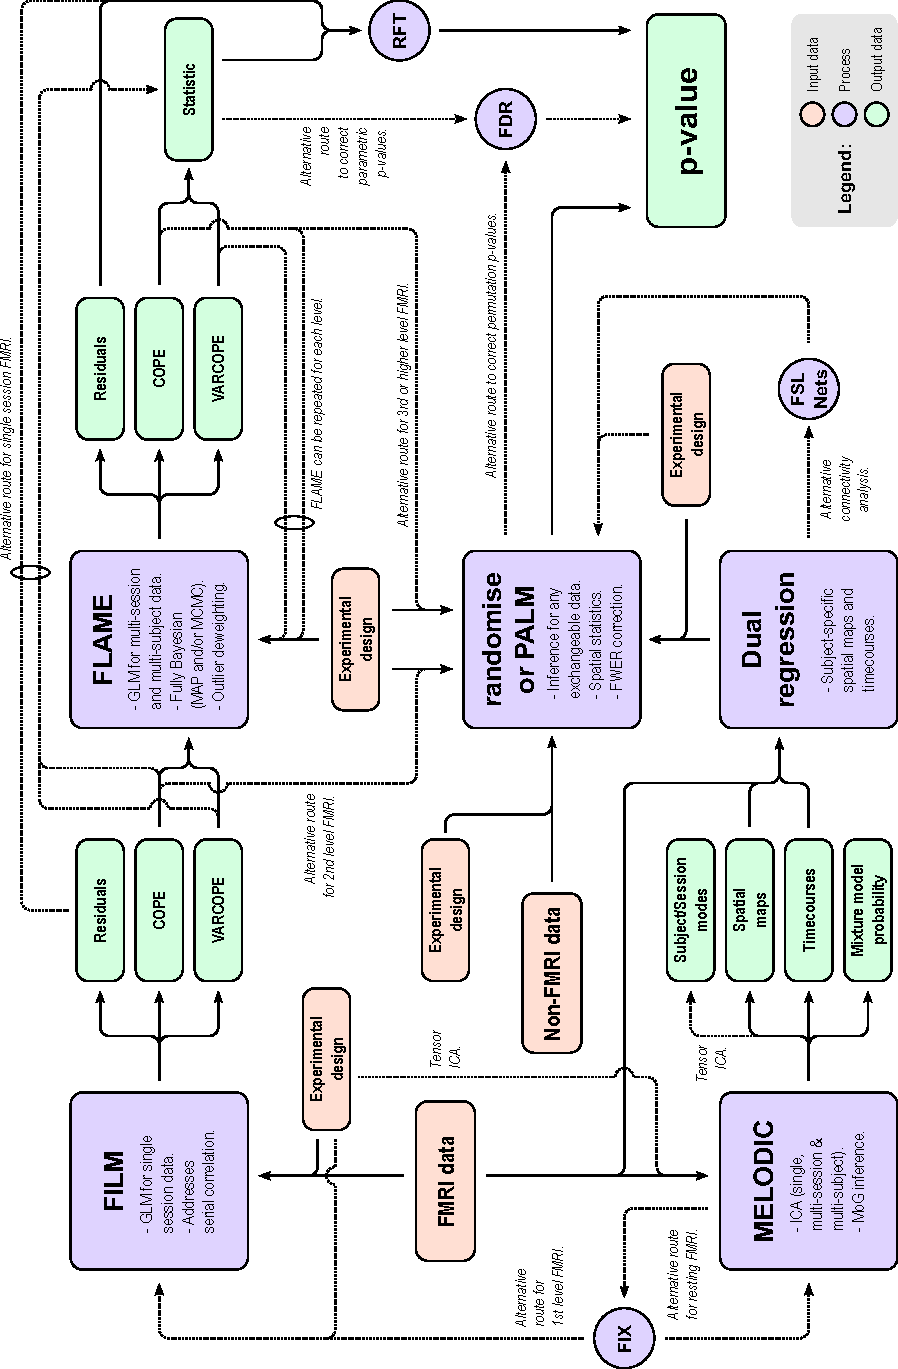
\includegraphics[width=\textwidth]{figures/fsl.pdf}
\end{center}
\label{fig:fsl_noref}
\end{figure}

In the example of \textsc{fsl}, although \texttt{randomise} already covers the most common types of experimental design, currently it does not address various other useful possibilities that include, for instance, (\textsc{i}) statistics that are robust to heteroscedasticity, (\textsc{ii}) multivariate methods, (\textsc{iii}) flexibility to accommodate designs with repeated measurements, (\textsc{iv}) correction for multiple testing based on minimal assumptions, not only across voxels, but also across multiple contrasts and multiple designs, (\textsc{v}) inference with missing data, (\textsc{vi}) multi-level inference on complete generality, for fixed-, random-, and mixed-effects, and (\textsc{vii}) all these performed in a reasonable amount of time even for large datasets. The absence of these techniques is not merely a lack of implementation in \textsc{fsl} or other software: some these topics have only been superficially covered by the literature, with even less work having addressed aspects that are specific to neuroimaging.

In this doctoral thesis, methods for the items (\textsc{iii}) and (\textsc{vii}) are introduced, thus widening the applicability of permutation tests to more cases than otherwise possible; the respective papers have been published \citep{Winkler2015, Winkler2016_fast}. Item (\textsc{i}) was discussed in \citet{Winkler2014}, which is not part of this thesis; likewise items (\textsc{ii}) and (\textsc{iv}) were presented in \citet{Winkler2016_npc}, also not part of this thesis. Items (\textsc{v}) and (\textsc{vi}) are left as future work. This thesis also explores an application of a permutation-based multivariate method, item (\textsc{ii}) above, using the theory presented in \citep{Winkler2016_npc} as the foundation that allows the replacement of analyses of the volume of the cerebral cortex for a joint analysis cortical thickness and cortical surface area. The respective paper is, at the time of this writing, under review, and a pre-print is publicly available in the \emph{bioRxiv} server \citep{Winkler2016_joint}.

Each chapter is a self-contained piece of work, under the common motif that is the extension of possible uses of permutation tests. Each individual chapter can be read together with the others or in isolation, although there is some intertextual elements, particularly on what concerns \textsc{npc}, that appears in Chapters \ref{sec:accel} and \ref{sec:cortex}. All three chapters build on previous research from the author, in particular \citet{Winkler2014, Winkler2016_npc}, but also, to some extent, \citet{Winkler2010, Winkler2012}. However, none of these readings are strictly necessary, and each chapter provides an introduction with a review of the relevant literature.

\subsection{Permutation under structured dependence}

In Chapter~\ref{sec:ptree} we propose a solution to a crucial problem that arises when using permutation tests for the analysis of experimental data using repeated measurements, which, depending on the hypothesis, violates exchangeability: the various measurements obtained from a given subject are not independent from each other, thus not exchangeable. Another case is for data such as those from the Human Connectome Project \citep[\textsc{hcp};][]{VanEssen2012,VanEssen2013}: as each subject does not constitute an independent observation --- many are twins, with additional siblings also participating of the study --- conventional permutation strategies, despite their superior properties in general, if used, would dangerously expose the researcher to an increased risk of false positives.

We address this problem by constructing the permutations in a way that respects the data structure, without the need to explicitly model such structure, by imposing restrictions on exchangeability. Observations are organised in blocks, which are nested within other blocks in a multi-level fashion; these blocks can be shuffled a whole, and inside them, sub-blocks are further allowed to be shuffled, in a recursive process. The method is flexible enough to accommodate permutations, sign-flippings \citep[sometimes also called \emph{wild bootstrap};][]{Guillaume2014}, and permutations together with sign-flippings. In particular, this permutation scheme allows the data such as those from the \textsc{hcp} to be analysed via permutations: subjects are allowed to be shuffled with their siblings while keeping the joint distribution intra-sibship maintained. Then each sibship is allowed to be shuffled with others of the same type, ultimately ensuring that the false positive rate is controlled at the level of the test.

The results from this chapter show that the error type \textsc{i} is controlled at the nominal level, and the power is just marginally smaller than that would be obtained by permuting freely if that were allowed. The more complex the block structure, the larger the reductions in power, although with large sample sizes, the difference reduces. Importantly, simply ignoring family structure in designs as this causes the error rates not to be controlled, with excess false positives, and invalid results. We show examples of false positives that can arise, even after correction for multiple testing, when testing associations between cortical thickness, cortical area, and measures of body size, such as height, weight, and body-mass index, all which are known to be highly heritable. Such false positives can be avoided with permutation tests that respect the family structure.

\subsection{Accelerating permutation tests}

For small sample sizes, low resolutions, or small regions of interest, a permutation test can run very quickly (in a matter of minutes with current personal computers). For larger data, however, they become computationally intensive, and accelerations become useful. The natural strategies to increase the speed consist of the use of faster computers, parallel processing, graphical processing units (\textsc{gpu}s), or use of optimised code. These are general methods that can be considered to various applications.

Instead, Chapter~\ref{sec:accel} does not build on such generic software or hardware improvements, but on properties of certain test statistics and other statistical devices. We evaluate six different strategies for acceleration --- some already existing in the literature, others introduced, improved, or adapted for brain imaging. These strategies allow accelerations larger two orders of magnitude, yielding nearly identical results as in the non-accelerated case. Some, such as tail approximation, are generic enough to be used in nearly all the most common scenarios, including univariate and multivariate tests, spatial statistics, and for correction for multiple testing.

In addition to accelerating the tests, some of these methods considered allow continuous p-values to be obtained, and refine them far into the tail of the distribution of the test statistic, thus avoiding the usual discreteness of p-values in permutation methods, which can be a problem in some applications if too few permutations are done. Based on the results of extensive simulations and on the reanalysis of previously published real data \citep{Douaud2007}, we provide a set of recommendations for cases in which each method should be preferred.

\subsection{Application to cortical morphometry}

A joint, combined analysis of multiple variables can be done using the \emph{non-parametric combination} (\textsc{npc}). While \textsc{npc} is only relatively new \citep{Pesarin2010}, its use in neuroimaging was impossible for two reasons: the need to store very large amounts of data, and low power caused by the fact that, in imaging, correction for multiple testing is mandatory. In a work unrelated to this thesis, \citet{Winkler2016_npc} have made modifications to the original \textsc{npc} so as to render it feasible, valid, and powerful for brain imaging, addressing specific details that include multiple testing and the treatment of spatial statistics.

In Chapter~\ref{sec:cortex}, the application of this modified \textsc{npc} to structural imaging reveals something quite remarkable: that there is a viable way to assess cortical volume that, differently than the wildly popular voxel-based morphometry (\textsc{vbm}), does not mirror the cortical surface area. More: the method is able to reveal patterns of cortical pathology that affect thickness and area in opposing directions --- something that \textsc{vbm} cannot do --- and that even jointly remain a directional test, i.e., not two-tailed, thus in contrast with classical tests such as \textsc{mancova}, which are unable disambiguate directional effects.

Given that thickness and surface area have quite recently been shown to reflect distinct biological processes, cortical volume could still find use for the study of disorders that affect both cortical area and thickness. Here we demonstrate that \textsc{npc} is a better suited solution, that remain superior even when employing an improved, analytic method to measure volume, that is also novel and introduced in this thesis, and that will become the default in the next major release of the FreeSurfer software package.

In the same chapter we also provide, obiter dictum, a comparison of the four existing methods for areal resampling, answering a well known question that had so far not been approached in the literature: can the simple nearest neighbour method for areal interpolation be trusted? The answer is a confident yes, provided that there is smoothing. This translates into substantial gains for those interested, as the alternative, exact method, is computationally too intensive. The chapter equips researchers focused in the in vivo study of cortical anatomy with the information necessary to make the best use of the state-of-the-art morphometry methods.
\cleardoublepage \chapter{Multi-level block permutation}
\label{sec:ptree}
\setstretch{\lspac}

\section{Introduction}

In the context of hypothesis testing using the general linear model (\textsc{glm}) \citep{Scheffe1959, Searle1971}, permutation tests can provide exact or approximately exact control of false positives, and allow the use of various non-standard statistics, all under weak and reasonable assumptions, mainly that the data are \emph{exchangeable} under the null hypothesis, that is, that the joint distribution of the error terms remains unaltered after permutation. Permutation tests that compare, for instance, groups of subjects, are of great value for neuroimaging \citep{Holmes1996, Nichols2002}, and in \citet{Winkler2014}, extensions were presented to more broadly allow tests in the form of a \textsc{glm}, and also to account for certain types of well structured non-independence between observations, which ordinarily would preclude the use of permutation methods. This was accomplished by redefining the basic exchangeable unit from each individual datum to blocks of data, i.e., rather than asserting exchangeability across all observations of a given experiment, blocks of exchangeable units are defined; these \emph{exchangeability blocks} (\textsc{eb}s) can be rearranged as a whole (\emph{whole-block exchangeability}), or the observations within block can be shuffled among themselves (\emph{within-block exchangeability}), using either permutations, sign flippings, or permutations combined with sign flippings.

In the same work, the $G$-statistic, a generalisation over various commonly used statistics, including the $F$-statistic, was proposed. $G$ is robust to known heteroscedasticity (i.e., the situation in which the variances are known to be not equal across all observations, which can be then classified into variance groups) and can be used with the \textsc{glm}, ensuring that pivotality is preserved, a crucial requisite for exact control over familywise error rate (\textsc{fwer}) using the distribution of the most extreme statistic \citep{Westfall1993}, as needed in many neuroimaging studies. A \emph{pivotal} statistic has a sampling distribution that does not depend on unknown parameters. Indeed, the use of \textsc{eb}s allows for variances to be heterogeneous, provided that the groups of observations sharing the same variance (i.e., \emph{variance groups}, \textsc{vg}s) \citep{Woolrich2004} are compatible with the \textsc{eb}s; specifically, for within-block exchangeability the \textsc{vg}s must coincide with the blocks, and for whole-block exchangeability they must include one or more observations from each block in a consistent order.

This arrangement, using a statistic that is robust to heteroscedasticity, the use of variance groups, and the imposition of restrictions on exchangeability through the use of \textsc{eb}s, allows inference on various designs that, otherwise, would be much more difficult to do non-parametrically. These designs include paired tests, longitudinal designs, and other common tests that involve repeated measurements. However, certain study designs, despite exhibiting well-structured dependence between observations, still cannot be accommodated in the above framework. This occurs when the overall covariance structure is known, but its exact magnitude is not. An example occurs when multiple measurements per subject are performed in more than one session, with more than one measurement per session: the measurements within session may be exchangeable, but not across sessions. Another example is for studies using siblings, such as designs using discordant sib-pairs (in which only one sibling is affected by a given disorder), or using twins: permutations that disrupt the constitution of any sibship cannot be performed, as this would violate exchangeability.

Studies such as these are relatively common, notably those that involve siblings. However, whereas in classical twin designs the central objective is to quantify the fraction of the variation in a measurement (trait) that can be explained by the familial relationship between subjects after potential confounds have been taken into account, a quantity known as \emph{heritability}, here the concern is with a general linear model, and the objective is to test the influence of explanatory variables on the observed data. In other words, the interest lies on the relationship between the covariates and the main trait, while the non-independence between observations, which is a feature of interest in a heritability study, is here a form of nuisance that imposes restrictions on exchangeability for permutation inference for the \textsc{glm}.

Rather than inadvertently breaking these restrictions, here we propose to test the null hypothesis using a subset of all otherwise possible permutations, only allowing the rearrangements that respect exchangeability, thus retaining original joint distribution unaltered. Exchangeability with respect to a subset of all possible permutations is termed \emph{weak exchangeability} \citep{Good2005}. For conciseness, we will use the solitary term ``exchangeability'', while making clear the subsets of permutations for which this is valid. As in our previous work, we treat observations or entire blocks of data as weakly exchangeable, but here we further extend the definition of \textsc{eb}s to allow more complex designs to be addressed. This is accomplished through the use of \emph{multi-level exchangeability blocks}, in which levels consist of \emph{nested} blocks; for each such block the state of within- or whole-block exchangeability can be specified. The blocks are defined hierarchically, based on information about the dependence within data, but not requiring the modelling of the actual dependency. Even though the possibility of using nested blocks was anticipated in \citet{Winkler2014} (``Whole-block and within-block can be mixed with each other in various levels of increasing complexity'', page 386), nothing further was studied or presented at the time. Here we provide a comprehensive description of the approach, investigate its performance, its power, and present an applied example using the data structure of the ongoing Human Connectome Project (\textsc{hcp}). In the Section \ref{sec:ptree:implementation}, we present an implementation strategy.

\section{Theory}

\subsection{Terminology}

When contrasting the method described in this chapter with simple data rearrangement, various terms could be adopted: \emph{single-level} vs.\ \emph{multi-level} block shuffling, emphasising the levels of relationship between observations; \emph{unrestricted} vs.\ \emph{restricted}, emphasising the imposition of restrictions on how the data are allowed to be rearranged at each shuffling; \emph{free} vs.\ \emph{tree} shuffling, emphasising the tree-like structure of the relationships between observations that allow shuffling. All these terms have equivalent meaning in the context of this chapter, and are used interchangeably throughout. The generic terms \emph{shuffling} and \emph{rearrangement} are used when the distinction between permutations, sign flippings or permutations with sign flippings is not relevant.

\subsection{Notation}
\label{sec:ptree:notation}

We consider a \textsc{glm} that can be expressed as $\mathbf{Y} = \mathbf{M}\boldsymbol{\psi} + \boldsymbol{\epsilon}$, where $\mathbf{Y}$ is the $N \times 1$ vector of observed data, $\mathbf{M}$ is the full-rank $N \times r$ design matrix that includes explanatory variables (i.e., effects of interest and possibly nuisance effects), $\boldsymbol{\psi}$ is the $r \times 1$ vector of $r$ regression coefficients, and $\boldsymbol{\epsilon}$ is the $N \times 1$ vector of random errors. Estimates for the $\boldsymbol{\psi}$ can be computed by ordinary least squares, i.e., $\boldsymbol{\hat{\psi}} = \mathbf{M}^{+}\mathbf{Y}$, where the superscript $(^{+})$ denotes a pseudo-inverse. One generally wants to test the null hypothesis that a given combination (contrast) of the elements in $\boldsymbol{\psi}$ equals to zero, that is, $\mathcal{H}_{0} : \mathbf{C}'\boldsymbol{\psi} = \boldsymbol{0}$, where $\mathbf{C}$ is a $r \times s$ full-rank matrix of $s$ contrasts, $1 \leqslant s \leqslant r$. The commonly used $F$ statistic can be computed as usual and used to test the null hypothesis. When $s = 1$, the Student's $t$ statistic can be computed as $t=\mathrm{sign}(\boldsymbol{\hat{\psi}})\sqrt{F}$. A p-value for the statistic is calculated by means of shuffling the data, the model, the residuals, or variants of these \citep[Table~2]{Winkler2014}. In any of these cases, to allow rearrangements of the data, some assumptions need to be made: either of \emph{exchangeable errors} (\textsc{ee}) or of \emph{independent and symmetric errors} (\textsc{ise}). The first allows permutations, the second sign flippings; if both are available for a given model, permutations and sign flippings can be performed together. These rearrangements are represented by permutation and/or sign flipping matrices $\mathbf{P}$, and the set of all such matrices allowed for a given design is denoted as $\mathcal{P}$.

At its simplest, the \textsc{eb}s for within- or whole-block exchangeability can be identified or represented by a set of indices $\{1$, $2$, \ldots, $B\}$, one for each of the $B$ blocks. A vector of size $N \times 1$, can be used to indicate to which \textsc{eb} each observation from $\mathbf{Y}$ belongs (Figure~\ref{fig:notation}, \emph{left}); an extra flag is passed to the shuffling algorithm (such as the \texttt{randomise} algorithm) to indicate whether the rearrangements of the data should happen as within- or as whole-block. While this notation probably covers the majority of the most common study designs, it allows only within- \emph{or} whole-block, but not \emph{both} simultaneously; in other words, if in a study the observations can be permuted within block, and the blocks as a whole can also be permuted, such notation does not convey all possibilities for reorganising the data while preserving their joint distribution unaltered, and algorithms would perform fewer shufflings than those that are effectively allowed.

\begin{figure}[!b]
\centering
\caption[Notations for the specification of exchangeability blocks.]{\emph{(page \pageref{fig:notation_noref})} Different notations for the specification of exchangeability blocks; in this example, 3 blocks of 3 observations each.
\emph{Top-left:} In a single-column notation, each block has its index (here 1, 2, and 3, shown in different, random colours for clarity), and either within- or whole-block exchangeability are possible, but not both simultaneously. The specification of which kind of shuffling is to be done requires extra information, as a flag passed to the algorithm that permutes the data.
\emph{Top-right:} In a multiple-column notation, that information is encoded by virtue of the indices having a sign indicating whether the exchangeable units of a block at a given level should be shuffled as a whole ($+$) or kept fixed ($-$); these are shown respectively in blue and red. The signs define whether it is possible to perform rearrangements within-block, or of the blocks as a whole, or both. The rightmost example serves only to illustrate the notation, and is not useful in practice as all the observations would need to remain still.
\emph{Middle:} Example permutations are shown, with the observation indices coloured for clarity.
\emph{Bottom:} Visual representations using a tree diagram. The levels can be depicted as branching from a central (top/central) node, akin to a tree in which the most peripheral elements (leaves) represent the observations. The nodes from which the branches depart can be labelled as allowing permutations $(+)$ or not $(-)$, shown respectively in blue and red colours. The letters (a) through (c) refer to the variance groups in Figure~\ref{fig:vargrps}.}
\label{fig:notation}
\end{figure}

\begin{figure}[!p]
\centering
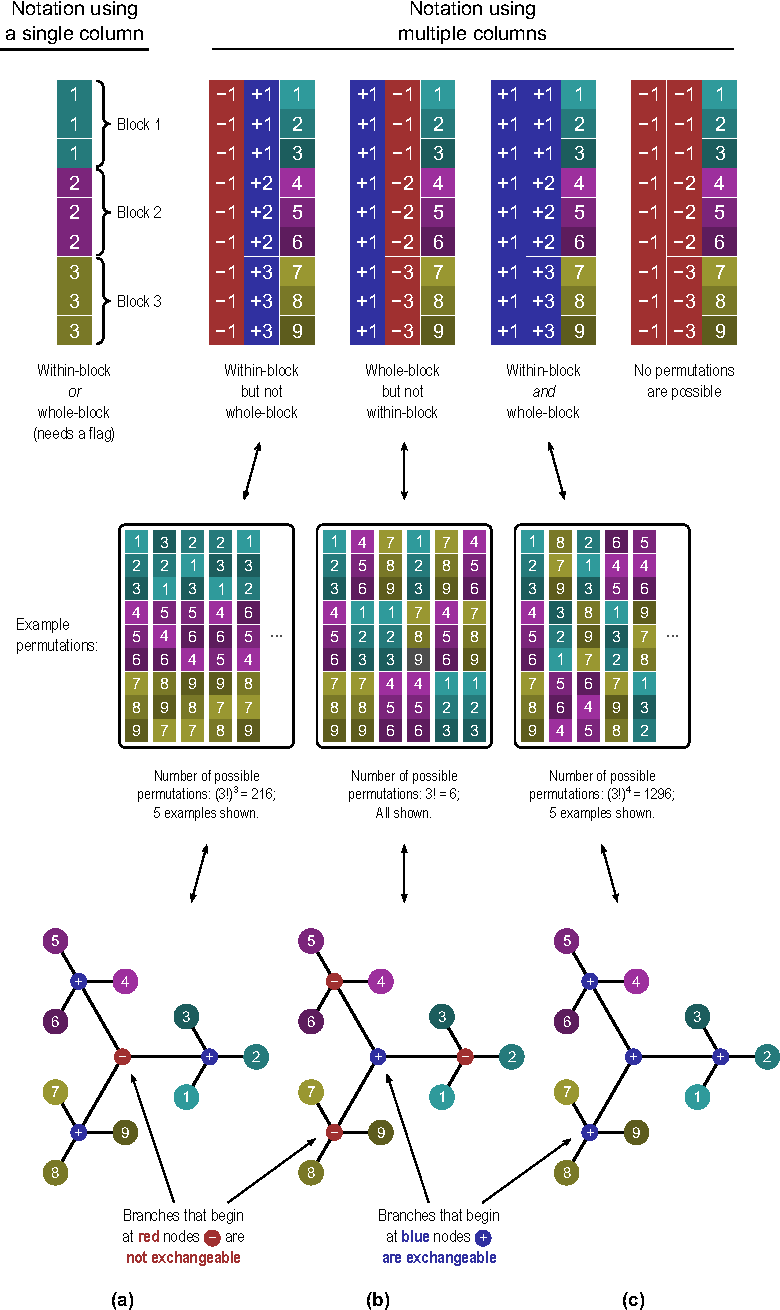
\includegraphics{figures/notation.pdf}
\label{fig:notation_noref}
\end{figure}

This can be addressed by extending the notation from a single column to a multi-column array, allowing nested \textsc{eb}s to be defined, such that blocks can contain sub-blocks, in a hierarchical fashion, and where each column represents a level; we use the leftward columns to indicate higher, and rightward to indicate lower levels. More columns alone, however, are not sufficient, because at each level, shufflings of observations or of sub-blocks can be allowed within-block, or the blocks at that level can be shuffled as a whole. Hence to discriminate between one type or the other, we use negative indices to indicate that the exchangeable units at the level immediately below should not be permuted, and positive indices indicate that shuffling of these units is allowed as usual (Figure~\ref{fig:notation}, \emph{right}). The exchangeable units can be sub-blocks, which can contain yet other sub-blocks, or observations if the next level immediately below is the last.

These two notations, i.e., using single- or multi-column indices, do not represent mathematical entities, and are not meant to be used for algebraic manipulation; rather, these notations are shorthand methods to represent structured relationships between observations. The covariance structure prevents unrestricted shuffling from being considered, but it often permits shufflings to happen in a certain orderly manner that preserves the joint distribution of the data. These notations are to be used by the algorithm that performs the test to construct the permutation and/or sign flipping matrices, which then can be used to effectively disarrange the model to construct the distribution of the statistic under the null hypothesis.

\subsection{Visual representation}

The notation using multiple columns encapsulates all the information necessary not only for the rearrangements to be constructed, but also to depict the relationships between the observations in a tree-like diagram, highlighting their hierarchy, as shown in the lower panel of Figure~\ref{fig:notation}. Branches can only be shuffled with each other if their size and internal covariance structure are perfectly identical; this information is contained in the signs and indices used to represent each block: positive indices (shown in blue) allow them to be permuted; negative (in red) prevent permutation and keeps the branches in their fixed positions. The permutation of branches at lower levels (when these exist) is controlled by the nodes at these lower levels, independently from those at higher levels or within the same level.

Using the tree diagram, it becomes clear that the terms ``within-block'' and ``whole-block'', that have been used so far to describe exchangeability and permutation strategies, become no longer necessary, as either the branches can be shuffled, or they cannot. It is also helpful in emphasising that more complicated designs can be considered using multi-level blocks, in which even the distinction between within- and  whole-block is softened, as each level in the multi-column notation is not restricted to contain purely positive or negative indices restricting (or not) the shuffling of their constituent sub-blocks (branches). These can be present alongside each other if immediately below a level in which shuffling is not allowed, such that some branches may be allowed to be shuffled, whereas others are not. It may also be the case that some levels need to be included in the notation only so that the number of levels remains the same across all branches of the tree, from the top node to the most distal (leaves), without affecting the construction of $\mathcal{P}$, but ensuring that the notation can be stored, without gaps, in a two-dimensional array; in the visual representation these are shown as small, sign-less nodes. Figure~\ref{fig:trees2} (\emph{left} and \emph{centre}) exemplifies these cases. Although the multi-column notation and the corresponding tree can become very complex, the simple, unrestricted exchangeability can also be accommodated, as shown in Figure~\ref{fig:trees2} (\emph{right}).

\begin{figure}[!tp]
\centering
\hspace*{0cm}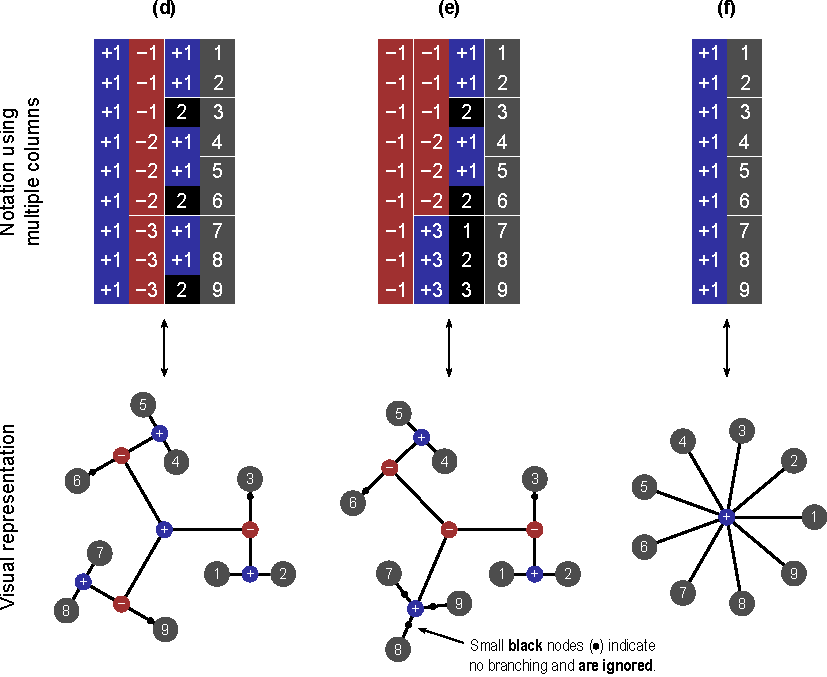
\includegraphics{figures/trees2.pdf}
\vspace{.3cm}
\caption[Complex, structured relationships between observations represented by multi-level exchangeability blocks.]{The multi-level definition of blocks allows more complex relationships between observations.
\emph{Left:} Three blocks of identical structure (2nd column) can be shuffled as a whole (as indicated by the positive indices in the 1st column); within each (3rd column), only two out of their three constituting observations can be swapped (1 and 2, 4 and 5, and 7 and 8), whereas the third on each (3, 6 and 9) cannot; levels for these last branches are completed with blocks for which the sign has no meaning (in black), as they remain unaltered towards the next level (4th column), and represent no actual branching. In the visual representation, these black blocks are shown as small black dots on continuous branches. This example could represent 3 sets of siblings, each composed of a pair of monozygotic twins and a third non-twin.
\emph{Centre:} An example showing that it is possible to mix types of blocks in the same level (2nd column). As shown, the first two blocks in the 2nd column cannot be swapped despite similar coding, and neither of these can be permuted with the third, which has a different structure consisting of three observations (7, 8 and 9) that can be shuffled freely. This example could represent 3 sets of siblings, the first a pair of monozygotic twins and a non-twin, the second a pair of dizygotic twins and a non-twin (if certain environmental effects are considered), and the third a set of three non-twin siblings.
\emph{Right:} The same notation can also accommodate simple designs. Here all 9 observations can be permuted without restrictions on exchangeability.}
\label{fig:trees2}
\end{figure}

\subsection{Variance groups and the $G$-statistic}

When the variances can be assumed to be the same throughout the sample, the classical $F$ and the Student's $t$ statistics can be used; these statistics have sampling distributions that do not depend on any unknown population parameters, but solely on the degrees of freedom, i.e., these are pivotal statistics. However, if homoscedasticity cannot be assumed, although $F$ and $t$ can still be used with permutation tests in general, they cannot be used to correct for multiple testing using the distribution of the most extreme statistic. The reason is that under heteroscedasticity, these statistics cease to be pivotal, and follow instead distributions that depend on the heterogeneous variances for the different groups of observations, causing them to be no longer adequate for \textsc{fwer} correction. Instead, a statistic that is robust to heteroscedasticity is necessary.

The $G$-statistic \citep{Winkler2014} was proposed to address this concern; this statistic is a generalisation of various other well established statistics, including $F$ and $t$, as well as the $v$-statistic used for the classical Behrens--Fisher problem. The definition of the variance groups used to calculate $G$ is based on knowledge about the data, and such groups need to be constructed together with the definition of the blocks. However, \textsc{vg}s and \textsc{eb}s represent different concepts; although they may coincide for simple designs, they do not need to. The \textsc{eb}s are used to indicate sets of observations that must remain together in every permutation due to having a non-diagonal \emph{covariance} structure, and are used by the permutation algorithm to rearrange the data many times to build the empirical distribution. The \textsc{vg}s, however, are used to indicate sets of observations that possess the same \emph{variance}, and are used to estimate the sample variance(s) when computing the statistic. Despite the distinction, any pair of observations that have the possibility of being swapped according to the \textsc{eb} structure must be in the same \textsc{vg}; observations in different variance groups cannot be permuted as that would modify the joint distribution, thus violating exchangeability.

For simple within-block permutation, the most restrictive configuration for the variance groups, that is, the configuration in which fewer observations need to be assumed to share the same variance, is such that each block corresponds to its own \textsc{vg}. For simple whole-block permutation, on the other hand, the first observation from each block, together, constitute a \textsc{vg}, the second observation from each block, together, another \textsc{vg}, and so forth. The minimum set of variance groups for more complicated designs can be derived similarly from the configuration of the exchangeability blocks; examples are shown in Figure~\ref{fig:vargrps}. The stringency of this definition lies in that, depending on the configuration of the \textsc{eb}s, each \textsc{vg} can contain only the smallest possible number of observations that can be assumed to have the same variance given the covariance structure imposed by the blocks. Such definition can, however, be relaxed by merging these minimum groups whenever homoscedasticity across more than one \textsc{vg} can be considered, while retaining the \textsc{eb}s unaltered. Whether merger, or any other definition, for the \textsc{vg}s should be sought for a given design may depend on information about the data or on the design itself. For a simple paired $t$-test, for instance, although each pair could in principle constitute a \textsc{vg} on its own, homogeneous variances can fairly well be assumed, with the benefit of much better variance estimates than would be obtained with groups of two sole observations.

Regardless of which strategy is used to define the variance groups, and irrespective of the indices used to represent each of them, the column vector containing these indices must be invariant with respect to the permutations that are allowed for a given design. In other words, let $\mathbf{v}$ be the column vector of length $N$ containing the indices that represent each variance group, such as those in Figure~\ref{fig:vargrps}. For any permutation matrix $\mathbf{P} \in \mathcal{P}$, $\mathbf{P}\mathbf{v}=\mathbf{v}$, that is, $\mathbf{v}$ is a common eigenvector for all permutation matrices in  $\mathcal{P}$. Any permutation that breaks this equality must not be used to test the null hypothesis, as this would mix observations that belong to different \textsc{vg}s, thus violating exchangeability. Likewise, a definition of groups that does not meet this criterion must not be used.

\begin{figure}[!tp]
\centering
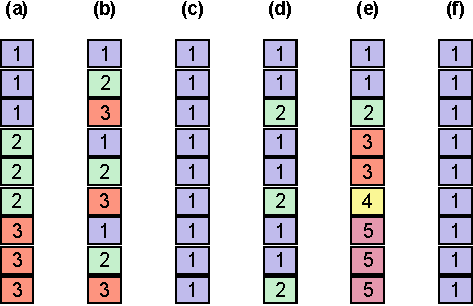
\includegraphics{figures/vargrps.pdf}
\vspace{1cm}
\caption[Variance groups defined from the exchangeability blocks.]{Variance groups defined from the exchangeability blocks (a)--(c) shown in Figure~\ref{fig:notation}, and (d)--(f) in Figure~\ref{fig:trees2}. These are the most restrictive configurations for the \textsc{vg}s that are possible given the structure imposed by the \textsc{eb}s. If, however, despite the covariance structure between observations, their variances are known to be or can be assumed to be homogeneous, some or all of these groups can be merged, with the additional benefit of improving the variance estimates. Alternatively, the groups can be entirely replaced by a different definition if additional information from the variance of the data is available. In (e), note two groups with only one observation each; see the main text for details.}
\label{fig:vargrps}
\end{figure}

\subsection{Number of permutations}

With the multi-level block permutation strategy, the rules to calculate the number of permutations are similar, yet more general than in the case of a single level that could be represented with a single-column notation. The number still depends on the number of repeated rows in the design matrix for methods as Manly and ter Braak \citep{Manly1986, terBraak1992} or, for methods as Draper--Stoneman and Freedman--Lane \citep{Draper1966, Freedman1983}, on the number of repeated rows across only the columns that are tested in the contrast after the model has been partitioned into effects of interest and nuisance effects.

Once the tree has been constructed, for the \textsc{ee} assumption, and in the absence of repetitions in the design as described above, the number of permutations can be calculated separately for each node in which shuffling is allowed as $B!$, with $B$ denoting the number of branches that begin at that node. If however, there are branches with identical structure and containing the repetitions in the design matrix, the number of possible permutations for that node is then $B!\left/\prod^{M}_{m=1}B_m!\right.$, where $M$ is the number of unique branches beginning at that node, and $B_m$ the number of times each of the $M$ unique branches begins at that node. The number of permutations for nodes that cannot be permuted is simply 1, that is, no permutation. With the number of permutations at each node calculated, the overall number of possible permutations for the whole design (whole tree) is the product of the number of possible permutations for all the nodes.

For \textsc{ise}, the number of sign flippings at the highest node in which shuffling is allowed is $2^B$, and 1 for all other nodes that lie below (distal) in the hierarchy. For the nodes in which shuffling is not allowed, the number of possible flips is 1, that is, no sign flippings are allowed, but it can still be higher than 1 for the nodes that lie below in the hierarchy. Unlike with permutations, the eventual presence of repeated elements in the design matrix does not affect the number of possible sign flippings. The number of possible sign flippings for the whole design is the product of the number of sign flippings for all the nodes.

When both \textsc{ee} and \textsc{ise} assumptions are valid for a given design, permutations can happen with sign flipping, and the total number of possible rearrangements is simply the product of the number of permutations with the number of sign flippings. Regardless of the kind of shuffling strategy adopted, the number of possible rearrangements can be extremely large, even for sample sizes of relatively moderate size. Not all of them need to be performed for the test to be valid and sufficiently exact; a random subset of all possible rearrangements can be sufficient for accurate hypotheses testing.

\subsection{Power}

The set of all rearrangements that can be performed while respecting the structure of the data is termed the \emph{permutation space} \citep{Pesarin2010}. The restrictions imposed by the \textsc{eb}s cause this space to be reduced, sometimes considerably, as none of the rearrangements that would violate exchangeability are performed. If the restrictions are such that the permutation space is not a representative, uniform sample from what the space would be without such restrictions, power may be reduced. In the Section~\ref{sec:ptree:evaluation} we assess various configurations for the multi-level \textsc{eb}s and their impact on the ability to detect true effects.

\subsection{Outliers}

Permutation tests strategies in general tend to be robust to outliers \citep{Anderson1999, Good2005}: although large outliers can bias the test statistic, the bias is present for all permutations; if a given outlier can be shuffled with \emph{any} other observation, their effect on the distribution of the test statistic tends to spread uniformly throughout its whole support. However, the dependence structure and the multi-level blocks may amplify the effect of outliers, since a given extreme value may no longer be shuffled with \emph{any} other observation, such that their their effect on the distribution of the test statistic may concentrate more strongly in some intervals than in others. The ultimate results then become difficult to predict, either in terms of conservativeness or anticonservativeness. Such problems may be minimised by providing some treatment of these extreme values; some possible remedies include censoring, trimming, replacement for ranks or quantiles, conversion of quantiles to a normal distribution, and robust regression.

\section{Implementation}
\label{sec:ptree:implementation}

\subsection{Permutation of the tree branches}

A na\"{i}ve way to select only the permutations that respect the data structure could be to create (randomly or lexicographically) permutation matrices as if the data could be shuffled freely, and then test whether these matrices would respect the configuration of the \textsc{eb}s at the various levels. If yes, the permutation matrix is used, otherwise it is discarded. The problem with this approach is not only that the process of testing can be slow, but also the restrictions imposed by the blocks can reduce the number of possible permutations by many orders of magnitude, implying that for some designs, for each valid permutation that is found, enormous numbers of permutations would need to be discarded, in a very inefficient process.

However, the diagram using a tree to represent the blocks and sub-blocks, and their hierarchical relationship, does not constitute merely a visual resource. The same tree structure can be used to efficiently implement a permutation algorithm that shuffles the branches, even in programming languages that do not offer natively a tree type, such as C or Octave/\textsc{matlab}, as trees can be constructed with pointers, or with generic types, such as cells. Figure \ref{fig:impltree_example} shows an example, further expanded in Figures \ref{fig:impltree_default} and \ref{fig:impltree_shuffled}. When constructing the tree representation, each node must store three pieces of information, which are all updated as the permutations and/or sign flips are performed. These three pieces are labelled as ``pieces'' in Figures \ref{fig:impltree_default} and \ref{fig:impltree_shuffled} (note the recursion), and described below:

\begin{figure}[!t]
\centering
\hspace*{0cm}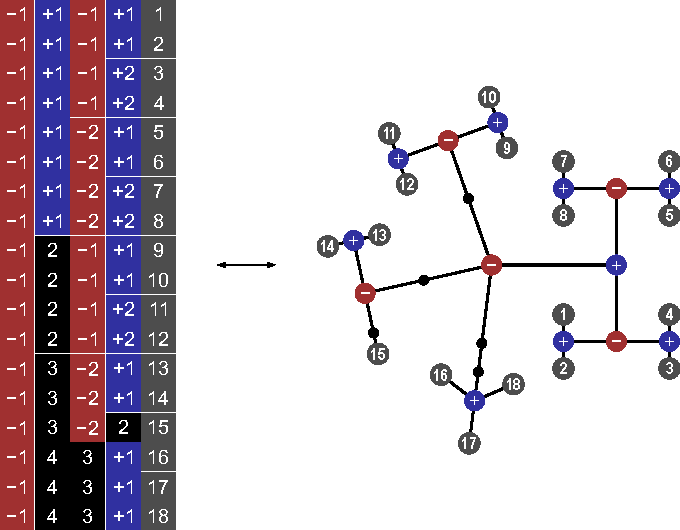
\includegraphics{figures/impltree_example.pdf}
\vspace{1cm}
\caption[An example multi-level block structure.]{An example multi-level block structure, to be compared with the example that illustrate the implementation; compare with Figures~\ref{fig:impltree_default} and \ref{fig:impltree_shuffled}, following the text description of the implementation strategy. (This is also the structure \textsc{d} shown in Figure~\ref{fig:treesCG}.)}
\label{fig:impltree_example}
\end{figure}

\begin{enumerate}
\item A three-column array, to be used under the \textsc{ee} assumption, and modified at each permutation, with as many rows as branches beginning at the node. The first column contains a sequence of integers that represents each of the branches. Branches that have identical structure and contain identical leaves (i.e., repeated rows in the relevant part of the design matrix necessary to test the null hypothesis) receive the same index and so this column can contain repeated values. This sequence is used by the Algorithm ``\textsc{l}'' \citep{Knuth2005}, the algorithm that performs lexicographic permutations without repetitions; as the algorithm runs, the rows are permuted as a whole. The second column contains the indices that represent the current permutation in relation to the original sequence, that is, the indices that rearrange the original sequence of branches into the current state after permuting. Reverse-indexing this sequence can reset the permuted branches back to the original, unpermuted state. The third column contains the indices that rearrange the previous state into the current state and, just before running the Algorithm ``\textsc{l}'' for the next permutation, this column is regenerated as a sequence $\{1$, $2$, \ldots, $B\}$, with $B$ here denoting the number of branches (sub-blocks) in the current level; these are the indices that effectively permute the branches. If branches that begin at the node cannot be permuted (negative indices in the multi-level block notation), the whole array is replaced by some distinct marker that can be tested quickly, such as a not-a-number (\texttt{NaN}) or simply a zero (0).
\item A vector of counters, to be used under the \textsc{ise} assumption. The counter can be in a numeral system of radix 2 (e.g., using $-1$ and $+1$ as symbols in lieu of the conventional binary 0 and 1), with as many digits as branches starting at the node, and representing in a direct manner the current state of the sign flippings for each branch that begin at that node. As in the case for permutations, if the signs in branches that begin at the node cannot be flipped, the vector of counters is replaced by a distinct marker, such as a not-a-number (\texttt{NaN}). For convenience, a the counter can be programmed using radix 10, then converted to radix 2 when the permutations are generated (in Figures \ref{fig:impltree_default} and \ref{fig:impltree_shuffled}, the vectors with the counters are shown in base 10).
\item The branches that begin at the node. Each branch is constituted of another tree structure, in a pattern that replicates itself recursively from the top level to the most distal branches.
\end{enumerate}

Once the tree has been constructed, shufflings can be performed exhaustively or, if the number of possible rearrangements is too large, only a subset needs to be performed. To generate any single permutation in lexicographic order, the tree is swept from the top node, proceeding recursively down to the next lower level before moving into the next branch in the same level, skipping the nodes in which the last lexicographic permutation has been reached (that is, the Algorithm ``\textsc{l}'' is unable to do any further shuffling), and stopping when a single pairwise permutation of branches can be performed. The respective branches are then swapped, all previous nodes already visited are reset back to their original, unpermuted state. A permutation vector is then constructed by concatenating the (now permuted) indices of the observations (leaves, at the far end of the tree), from which the permutation matrix is generated.

For sign flippings, the process is similar: the tree is swept in a similar order, but instead of computing the next permutation, the counter for a particular branch is incremented. Nodes that have reached the last possible sign flipping (i.e., with all signs reversed) are skipped; when a node can have its counter incremented, the sweeping stops, the counter is incremented by one, and all previous nodes that had been skipped are reset back to their original state. As the counter uses a numeral system with base 2, the counter itself constitutes a vector of sign flips that can be applied to the branches that begin at that node, and generating the sign flipping matrix is then trivial.

\begin{figure}[!b]
\caption[The multi-level structure used in the implementation, at the first permutation.]{\emph{(page \pageref{fig:impltree_default_noref})} An example of a multi-level tree structure, showing the elements used in the implementation, at the first permutation, in which all the terminal leaves (observation indices) are in their original position, and no sign flippings have been performed. At each level, three ``pieces'' of information are present, the third one being, recursively, another such level. Compare with Figure \ref{fig:impltree_example} and the text for a complete description.}
\label{fig:impltree_default}
\end{figure}

\begin{figure}[!b]
\caption[The multi-level structure used in the implementation, after random shufflings.]{\emph{(page \pageref{fig:impltree_shuffled_noref})} The same example multi-level structure shown in Figure \ref{fig:impltree_shuffled}, after random permutations of branches and sign flippings have been performed.}
\label{fig:impltree_shuffled}
\end{figure}

\begin{figure}[!p]
\centering
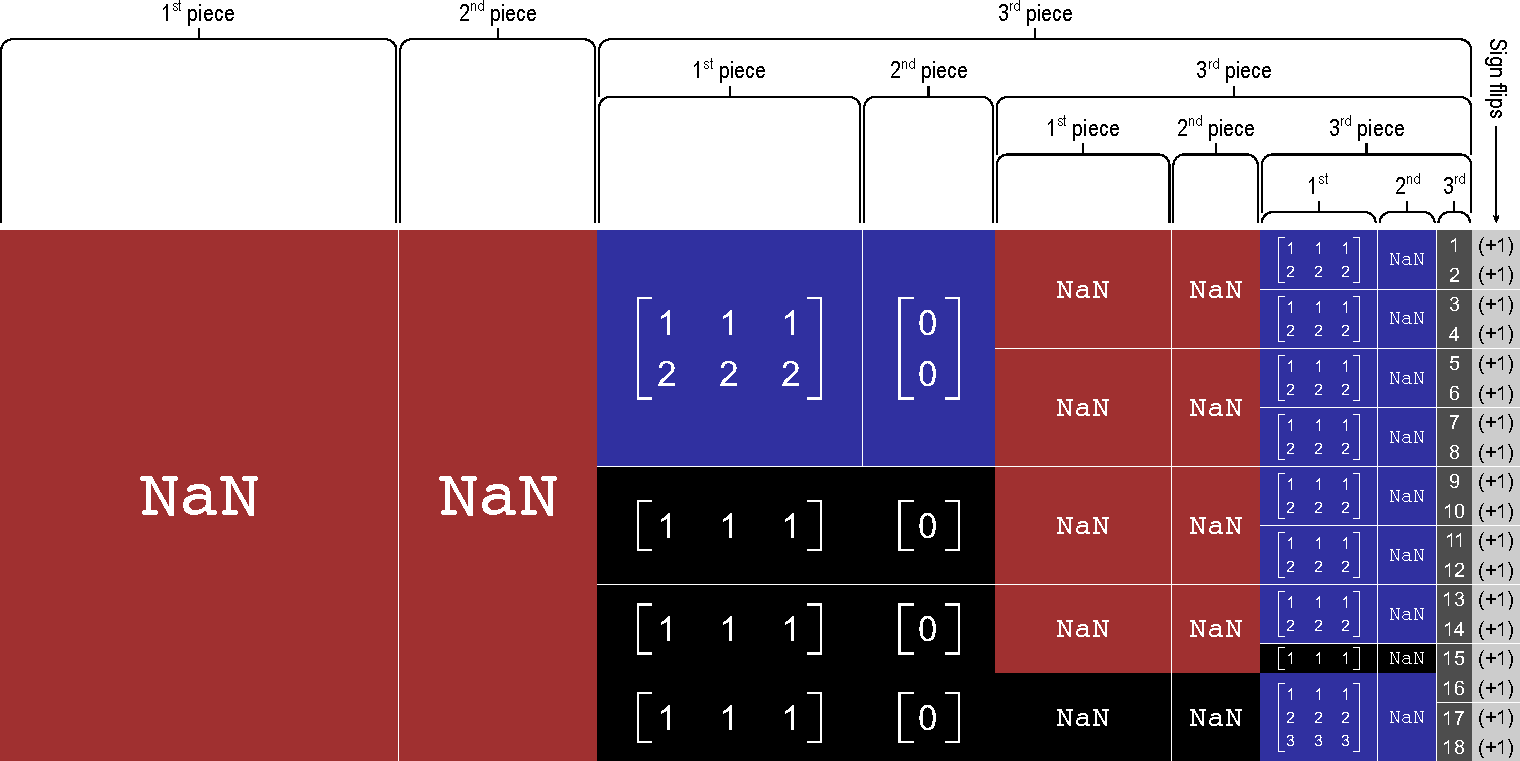
\includegraphics[angle=90,origin=c,scale=.8]{figures/impltree_default.pdf}
\label{fig:impltree_default_noref}
\end{figure}

\begin{figure}[!p]
\centering
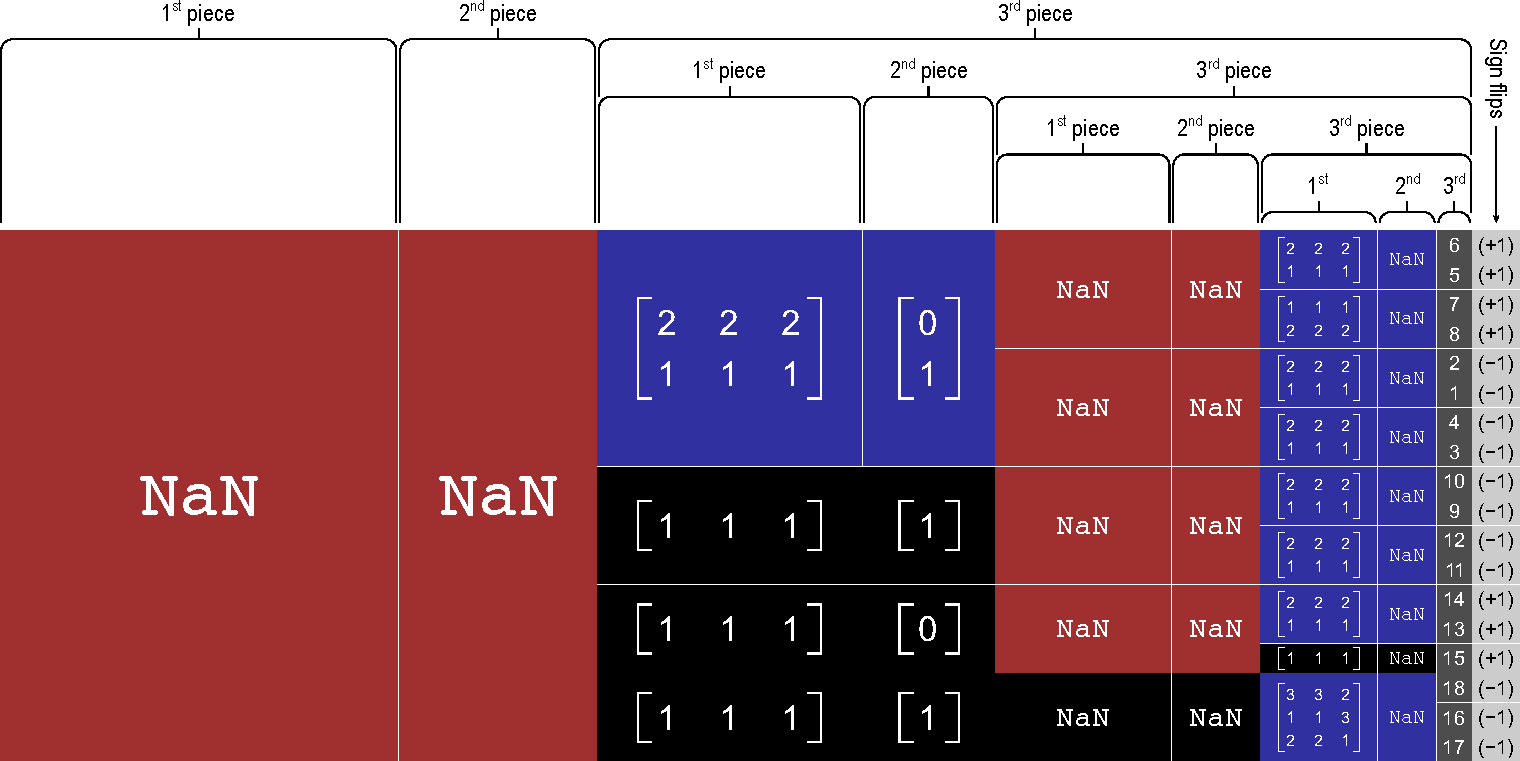
\includegraphics[angle=90,origin=c,scale=.8]{figures/impltree_shuffled.pdf}
\label{fig:impltree_shuffled_noref}
\end{figure}

As described, the tree representation allows computing exhaustively and lexicographically all possible rearrangements. However, the tree can also be perturbed randomly, with the branches that begin in all its nodes being permuted and/or sign flipped, a feature useful when performing only a small subset of all possible shufflings.

\subsection{Variance groups}

The most restrictive set of \textsc{vg}s can also be defined from the same tree structure. The nodes of the tree are swept from the first branch in the top node, proceeding recursively down to the next lower level before moving into the next branch in the same level. At the lowest level, observations (leaves) that can be permuted are assigned to the same variance group; those that cannot are each assigned to a distinct group. At the intermediate nodes, between the top node and the terminal leaves, those in which permutation of the branches is allowed have their corresponding \textsc{vg}s defined for the first branch, then replicated for all remaining branches at that level without the need to visit their lower levels. For the nodes in which permutation of branches is not allowed, each branch has its own set of \textsc{vg}s defined. A counter is passed down and up the levels as each node is visited, being incremented to the next integer every time a new \textsc{vg} is created.

Actual code for the above implementation, including the assembly of the tree, its shuffling using permutations and/or sign flippings, with complete enumeration in lexicographic order using the Algorithm ``\textsc{l}'', as well as generation of the variance groups, all written in \textsc{matlab}, is available in the tool \textsc{palm} -- Permutation Analysis of Linear Models; consult Section \ref{sec:conclusion:palm} for details.

\section{Evaluation method}
\label{sec:ptree:evaluation}

\subsection{Error rates and power}

The error rate is calculated as the proportion of tests that are significant when there is no effect. Power is calculated as the proportion of tests that are significant when a true effect is present. In either case, it is necessary to know whether true effects are present or not. Moreover, multiple realisations are necessary for the proportions to be calculated. In the simulations below, two dependence structures, named datasets \textsc{a} and \textsc{b}, were created to evaluate the permutation strategy. Both use mixtures of levels that can or that cannot be shuffled. For the dataset \textsc{a}, $N=36$ observations were simulated, grouped into nine exchangeability blocks of four observations each, and each of these further divided into two blocks of two. Not all levels were allowed to be shuffled freely, and the structure is shown in Figure~\ref{fig:treesAB} (\emph{left}). For dataset \textsc{b}, $N=27$ observations were divided into nine \textsc{eb}s of three observations each; and each of these further divided into two blocks, one with two, and one with one observation, as shown in Figure~\ref{fig:treesAB} (\emph{right}). Although these may appear somewhat artificial for practical use, we wanted examples that would restrict the number of possible shufflings, to test the multi-level strategy in relatively difficult scenarios. The structure in dataset \textsc{a} precisely emulates a twin study with nine sets of siblings, each comprised of a pair of monozygotic twins and a pair of non-twins (or of dizygotic twins). Dataset \textsc{b} uses a similar scheme, but further restricts the possibilities for shuffling by having just one non-twin in each set of siblings.

\begin{figure}[!p]
\centering
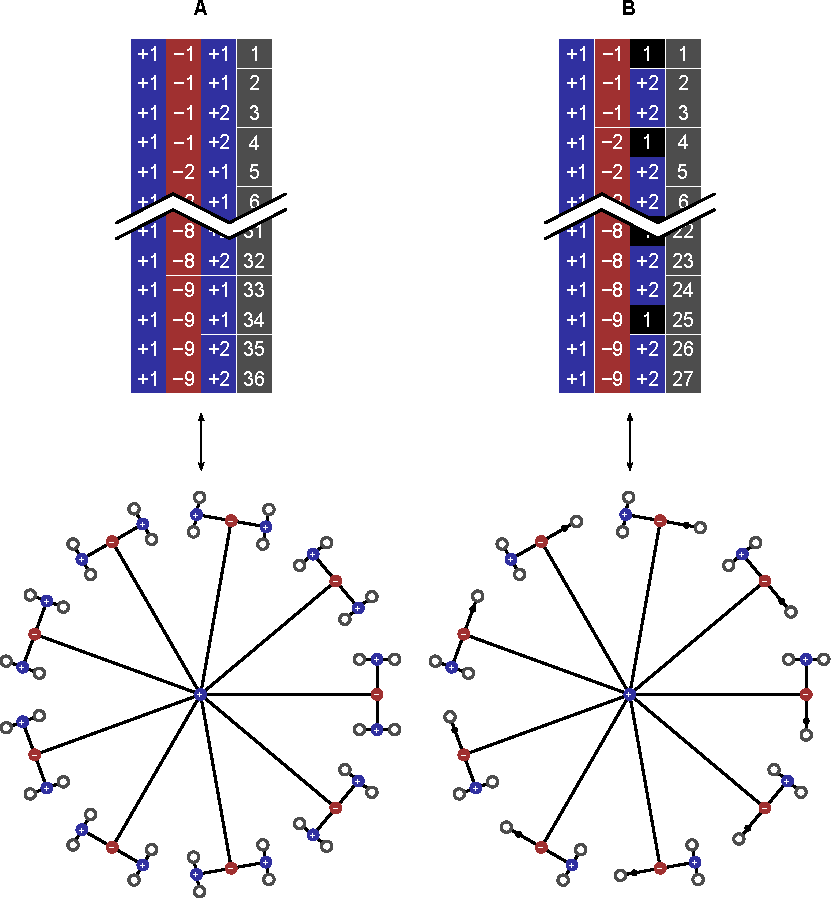
\includegraphics{figures/treesAB.pdf}
\vspace{1cm}
\caption[The two simulated dependence structures used to assess error rates and power.]{The two dependence structures, \textsc{a} and \textsc{b}, used to assess error rates and power.
\emph{Top:} Multi-level block definition.
\emph{Bottom:} Visualisation as a tree diagram.} 
\label{fig:treesAB}
\end{figure}

Using the same notation as in Section \ref{sec:ptree:notation}, 500 response variables (data vectors $\mathbf{Y}$) were simulated for each dataset, using the model $\mathbf{Y} = \mathbf{M}\boldsymbol{\psi} + \boldsymbol{\epsilon}$; each variable might represent, for instance, a voxel or vertex in a brain image. The residuals, $\boldsymbol{\epsilon}$, were simulated following either a Gaussian distribution (with zero mean and unit variance), a Weibull distribution (skewed, with scale parameter 1 and shape parameter 1/3, shifted and scaled so as to have expected zero mean and unit variance), or a Laplace distribution (kurtotic, with zero mean and unit variance)\footnote{The actual skewness and kurtosis for these two distributions are either fixed or functions of their parameters, and therefore were held constant throughout the simulations. For Weibull, the skewness is $\left(\Gamma\left(1+3/k\right)\lambda^3-3\mu\sigma^2-\mu^3\right)\left/\sigma^3\right. \approx 19.58$, where $k$ is the shape and $\lambda$ the scale parameter. For Laplace, the excess kurtosis is $3$.}. In order to introduce dependence between the residuals, for simplicity and without loss of generality to any study in which there is dependence among the data, including repeated measurements, each observation was treated as if from a participant in a twin study design, as described above, and an $N \times N$ correlation matrix $\boldsymbol{\Omega}$, was created using the coefficient of kinship, $2\phi_{ij}$, between subjects $i$ and $j$ \citep{Jacquard1970}, such that $\boldsymbol{\Omega}=2\boldsymbol{\Phi}h_{\boldsymbol{\epsilon}}^{2} + \mathbf{I}(1-h_{\boldsymbol{\epsilon}}^{2})$, where $\boldsymbol{\Phi}$ is the matrix with the coefficients $\phi_{ij}$, and $\mathbf{I}$ is the identity matrix. The benefit of constructing the simulations in this way is that the strength of the dependence structure can vary linearly in the interval 0 to 1 using a single parameter, here denoted as $h_{\boldsymbol{\epsilon}}^{2}$, which coincides, in quantitative genetics and under certain assumptions, with the heritability of the measurement after explanatory or nuisance variables have been considered. The coefficient of kinship ($2\phi_{ij}$) is set to 1 for monozygotic twins, 0.5 full siblings that are not monozygotic twins, 0.25 for half siblings, and 0 for unrelated subjects. For these simulations, we used different values for the heritability of the residuals as $h_{\boldsymbol{\epsilon}}^{2}$ $=$ $\{0,$ $0.4,$ $0.8\}$. To introduce the desired correlation structure, $\boldsymbol{\Omega}$ was subjected to a Cholesky decomposition such that $\boldsymbol{\Omega}=\mathbf{L}'\mathbf{L}$, then redefining the residuals as $\mathbf{L}'\boldsymbol{\epsilon}$.

The dependent data, $\mathbf{Y}$, were generated by adding the simulated effects, $\mathbf{M}\boldsymbol{\psi}$, to the residuals, $\boldsymbol{\epsilon}$, with $\boldsymbol{\psi}$ $=$ $[\psi_1 \; 0]'$, $\psi_1$ being either 0 or:
$$t^{-1}_{\text{cdf}}\left(1-\alpha ; N-\mathrm{rank}\left(\mathbf{M}\right)\right)\left/\sqrt{N}\right.$$
where $\alpha$ $=$ $0.05$ is the significance level of the permutation test to be performed at a later stage, ensuring a calibrated signal strength sufficient to yield an approximate power of 50\% with Gaussian errors, irrespective of the sample size. The actual effect was coded in the first regressor only, here denoted $\mathbf{m}$, the second regressor modelling an intercept. This regressor was constructed as a set of random values following a Gaussian distribution with zero mean and unit variance. As in real experiments, such effects of interest may be (as with the residuals) not independent across observations, three different values for the strength of this dependence were simulated, using $h_{\mathbf{m}}^{2}$ $=$ $\{0,$ $0.4,$ $0.8\}$. These values are equivalent to the heritability of $\mathbf{m}$ in the context of genetics, yet without loss of generality to studies in which there is dependence between the data that constitute any individual independent variable, including certain designs involving repeated measurements.

Permutations, sign flippings, and permutations with sign flippings were performed, either freely or respecting the dependence structure. In each case, 500 shufflings were performed for each of the 500 variables, and the whole process was repeated 500 times, allowing histograms of p-values to be constructed, as well as to estimate the variability around the heights of the histogram bars. Confidence intervals (95\%) were computed for the empirical error rates and power using the Wilson method \citep{Wilson1927}. Significance levels were also compared using Bland--Altman plots \citep{Bland1986}, modified so as to include the confidence intervals around the means of the methods.

\subsection{Power}

The evaluations above were used to assess error rates and power according to the degree of non-independence between observations and distribution of the errors. To further investigate how the restrictions imposed by the exchangeability blocks could affect power, other dependence structures were considered to shuffle the data, in addition to the datasets \textsc{a} and \textsc{b} above; these were named \textsc{c} through \textsc{i} (Figures~\ref{fig:treesCG}, \ref{fig:treeHCP_full}, and \ref{fig:treeHCP_dz2sib}). The configuration \textsc{c} corresponds to freely shuffling 11 observations; \textsc{d} corresponds to a small set of 5 sibships with a total of 18 subjects, mixing whole-block and within-block at different levels; \textsc{e} is formed by 15 observations, organised in 5 blocks of 3 observations each, with shufflings being allowed within-block only; \textsc{f} is similar, but with whole-block rearrangements only, and \textsc{g} also similar, but allowing both whole-block and within-block simultaneously; configurations \textsc{h} and \textsc{i} use the family structure of the Human Connectome Project at the time of the \textsc{hcp-s}500 release (more details below): in \textsc{h}, dizygotic twins are treated as a category on its own, thus accounting for the possibility of shared, non-genetic effects within twin pair, whereas in \textsc{i}, dizygotic twins are treated as ordinary, non-twin full siblings. The number of possible permutations and sign flippings for each of these structures is shown in Table~\ref{tab:nperms}.

\begin{figure}[!tp]
\centering
\hspace*{0cm}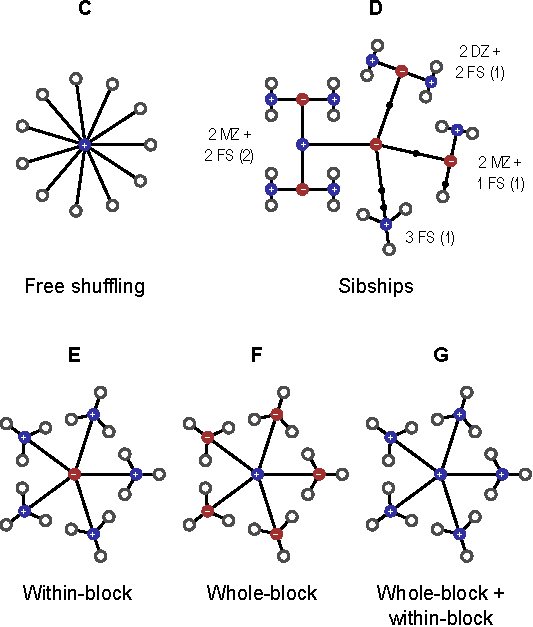
\includegraphics{figures/treesCG.pdf}
\vspace{1cm}
\caption[Tree diagrams used to assess power.]{Tree diagrams \textsc{c}--\textsc{g}, used to assess power, in addition to \textsc{a}, \textsc{b}, textsc{h} and \textsc{i} (shown in Figures~\ref{fig:treesAB}, \ref{fig:treeHCP_full} and \ref{fig:treeHCP_dz2sib}). In \textsc{c}, observations can be shuffled without restrictions. In \textsc{d}, which represent a set of five sibships, \textsc{mz} refers to each subject of a pair of monozygotic twins, \textsc{dz} to dizygotic twins, and \textsc{fs} to full siblings (non-twin and not half siblings); the numbers in parentheses indicate the number of each type of sibship in the tree (see also Figure~\ref{fig:treeHCP_full}). In \textsc{e}, observations can be shuffled only within-block; in \textsc{f} the blocks as a whole can be shuffled, and in \textsc{g}, shufflings are allowed within-block, and the blocks as a whole can also be shuffled.}
\label{fig:treesCG}
\end{figure}

\begin{figure}[!tp]
\centering
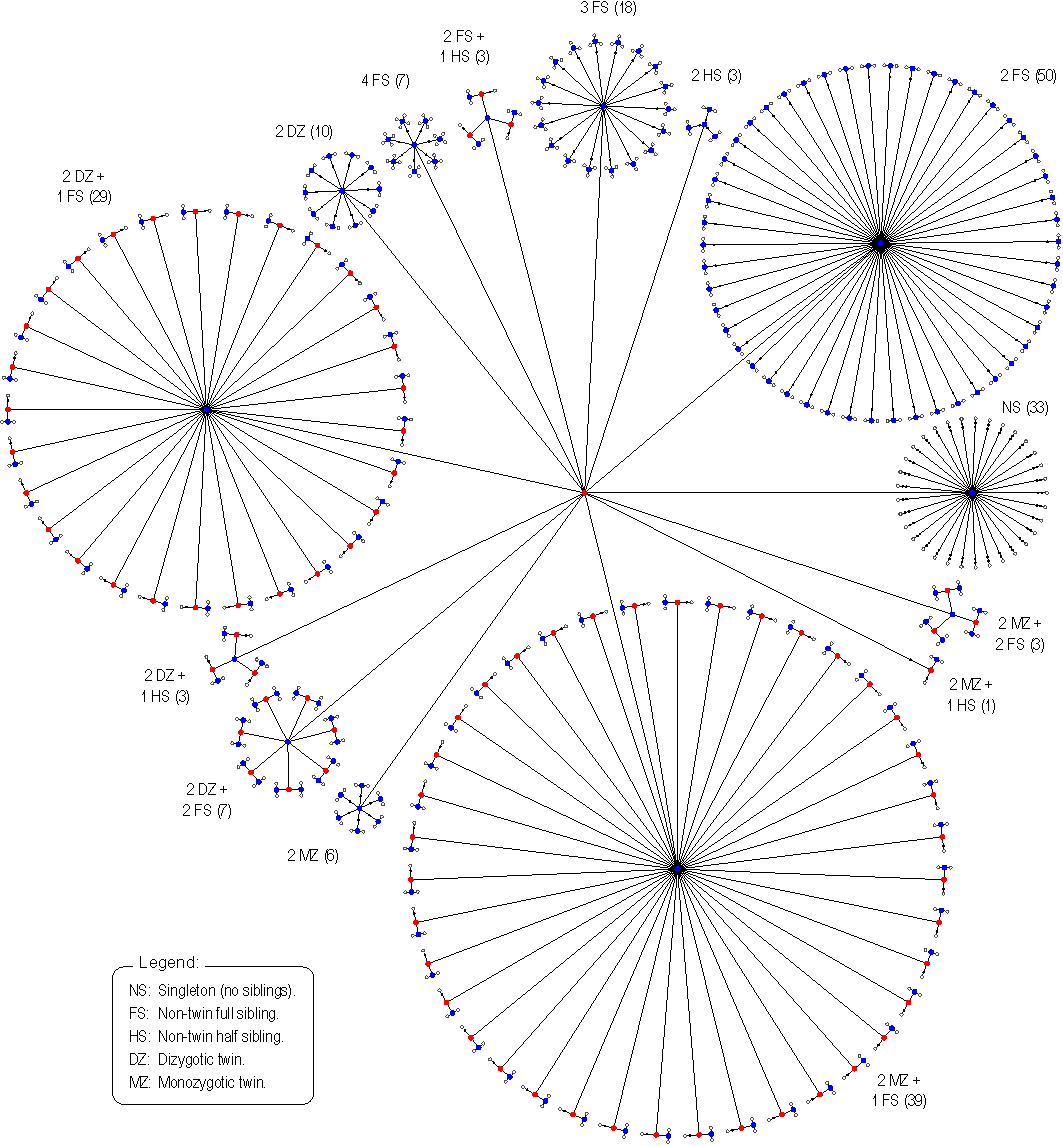
\includegraphics[scale=.75]{figures/treeHCP_full.pdf}
\vspace{5mm}
\caption[Tree diagram for \textsc{hcp} subjects.]{Tree diagram depicting the structure present among the subjects of the Human Connectome Project \textsc{hcp}, at the time of the release \textsc{hcp-s500}, with 518 subjects. The numbers in parentheses indicate how many of each type of sibship set are present.}
\label{fig:treeHCP_full}
\end{figure}

\begin{figure}[!tp]
\centering
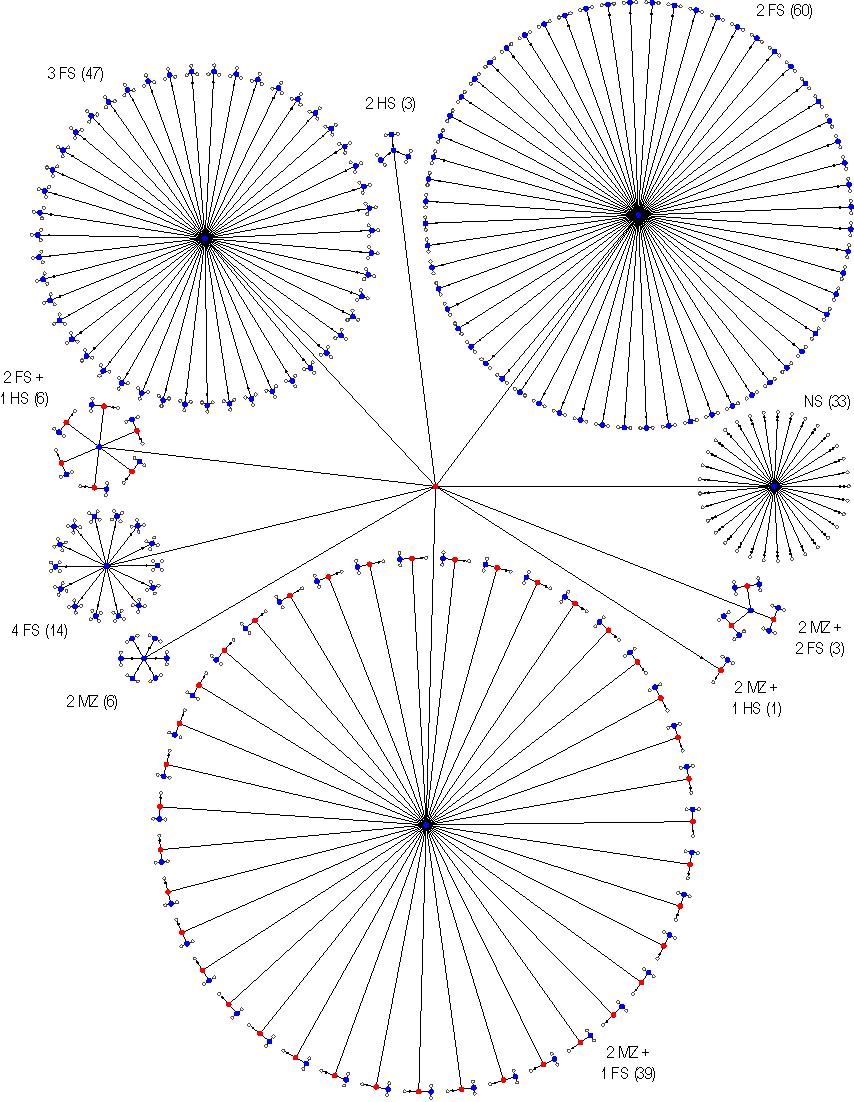
\includegraphics[scale=.75]{figures/treeHCP_dz2sib.pdf}
\vspace{5mm}
\caption[Tree diagram for \textsc{hcp} subjects, with dizygotic twins as ordinary siblings.]{Tree diagram representing the structure among the same 518 subjects of the \textsc{hcp-s500} release, shown in Figure~\ref{fig:treeHCP_full}, but treating dizygotic twins as ordinary siblings, therefore not accounting for the possibility of shared common non-genetic effects within dizygotic twin pair.}
\label{fig:treeHCP_dz2sib}
\end{figure}

\begin{table}[!tp]
\caption[Number of permutations and sign flippings for the dependence structures used to examine power.]{Number of permutations (\textsc{ee}) and sign flippings (\textsc{ise}) for the 9 dependence structures simulated to examine power. If there were ties in the data, the number of possible permutations would be smaller. When both \textsc{ee} and \textsc{ise} can be used, such that the data can be permuted and sign flipped, the number of possible rearrangements is simply the product of the number of permutations with the number of sign flippings. The footnote shows in detail how these values were calculated for the more complex configurations.}
\begin{center}
{\small
\begin{tabular}{@{}m{10mm}<{\raggedright}
                   m{29mm}<{\raggedright}
                   m{28mm}<{\raggedright}
                   m{29mm}<{\raggedright}
                   m{23mm}<{\raggedright}@{}}
\toprule
{}        & \multicolumn{2}{c}{Unrestricted shuffling} & \multicolumn{2}{c}{Restricted shuffling}\\
\cmidrule(lr){2-3} \cmidrule(l){4-5}
Set & \textsc{ee} & \textsc{ise} & \textsc{ee} & \textsc{ise}\\
\midrule
\textsc{a} & $36! \approx 3.7 \cdot 10^{41}$ & $2^{36} \approx 6.9 \cdot 10^{10}$ & $4^9 \cdot 9! \approx 9.5 \cdot 10^{10} $ & $2^9=512$\\
\textsc{b} & $27! \approx 1.1 \cdot 10^{28}$ & $2^{27} \approx 1.3 \cdot 10^{8}$ & $2^9 \cdot 9! \approx 1.9 \cdot 10^{8} $ & $2^9=512$\\
\textsc{c} & $11! \approx 4.0 \cdot 10^{7}$ & $2^{11} = 2048$ & $11! \approx 4.0 \cdot 10^{7}$ & $2^{11} = 2048$\\
\textsc{d} & $18! \approx 6.4 \cdot 10^{15}$ & $2^{18} = 262144$ & $2^8 \cdot 3! = 1536$ & $2^5 = 32$\\
\textsc{e} & $15! \approx 1.3 \cdot 10^{12}$ & $2^{15} = 32768$ & $(3!)^5 = 7776$ & $2^{15} = 32768$\\
\textsc{f} & $15! \approx 1.3 \cdot 10^{12}$ & $2^{15} = 32768$ & $5! = 120$ & $2^5 = 32$\\
\textsc{g} & $15! \approx 1.3 \cdot 10^{12}$ & $2^{15} = 32768$ & $(3!)^5 \cdot 5! = 933120$ & $2^5 = 32$\\
\textsc{h} & $518! \approx 6.5 \cdot 10^{1182}$ & $2^{518} \approx 8.6 \cdot 10^{155}$ & $a \approx 2.9 \cdot 10^{287}$ & $c \approx 6.6 \cdot 10^{63}$\\
\textsc{i} & $518! \approx 6.5 \cdot 10^{1182}$ & $2^{518} \approx 8.6 \cdot 10^{155}$ & $b \approx 1.3 \cdot 10^{335}$ & $d \approx 6.6 \cdot 10^{63}$\\
\bottomrule
\end{tabular}}
\end{center}
{\scriptsize
\begin{enumerate}
\item[$a \; =$] $[33!] \cdot [2^{50} \cdot 50!] \cdot [2^{3} \cdot 3!] \cdot [(3!)^{18} \cdot 18!] \cdot [2^3 \cdot 3!] \cdot [(4!)^7 \cdot 7!] \cdot [2^{10} \cdot 10!] \cdot [2^{29} \cdot 29!] \cdot [2^3 \cdot 3!] \cdot [(2^2)^7 \cdot 7!] \cdot [2^6 \cdot 6!] \cdot [2^{39} \cdot 39!] \cdot [2] \cdot [(2^2)^3 \cdot 3!]$.
\item[$b \; =$] $[33!] \cdot [2^{60} \cdot 60!] \cdot [2^3 \cdot 3!] \cdot [(3!)^{47} \cdot 47!] \cdot [2^6 \cdot 6!] \cdot [(4!)^{14} \cdot 14!] \cdot [2^6 \cdot 6!] \cdot [2^{39} \cdot 39!] \cdot [2] \cdot [(2^2)^3 \cdot 3!]$.
\item[$c \; =$] $2^{33} \cdot 2^{50} \cdot 2^{3} \cdot 2^{18} \cdot 2^{3} \cdot 2^{7} \cdot 2^{10} \cdot 2^{29} \cdot 2^{3} \cdot 2^{7} \cdot 2^{6} \cdot 2^{39} \cdot 2 \cdot 2^{3} = 2^{212}$.
\item[$d \; =$] $2^{33} \cdot 2^{60} \cdot 2^{3} \cdot 2^{47} \cdot 2^{6} \cdot 2^{14} \cdot 2^{6} \cdot 2^{39} \cdot 2 \cdot 2^{3} = 2^{212}$.
\end{enumerate}
Compare products $a$, $b$, $c$ and $d$ with Figures~\ref{fig:treeHCP_full} and \ref{fig:treeHCP_dz2sib}, that depict respectively the \textsc{hcp} structures \textsc{h} and \textsc{i}; the factors are shown starting from the singletons (labelled as \textsc{ns} in the figures) and running counter-clockwise around the central node.\par}
\label{tab:nperms}
\end{table}

For each of these nine datasets, an artificial effect (signal) was introduced, in the same way as described in the previous section, but here exclusively using independent Gaussian errors and preserving this independence throughout the simulations while still using multi-level exchangeability blocks for shuffling, as if dependencies among the data existed. Power was then compared with what would be observed if the same data were shuffled without the restrictions imposed by the \textsc{eb}s. For each configuration, 100 repetitions were performed, each simulating 1000 variables (as before, each could represent a voxel or vertex in an image). Up to 512 shufflings were used, either permutations, sign flippings, or permutations with sign flippings. Each repetition used a different set of random observations and a different set of shufflings when the maximum number of possible rearrangements was larger than the number of shufflings performed. The significance level was set as $\alpha$ $=$ $\sfrac{1}{16}$ $=$ $0.0625$. Both the number of permutations and the significance level were chosen so as to allow compatible resolutions of the p-values among runs, allowing a more direct comparison between each case.

Power changes were assessed in relation to what would be observed if the data were shuffled freely, and compared to a measure of the amount of shuffling applied to the data, given the restrictions imposed by the permutation tree. For this purpose, Hamming distance \citep{Hamming1950} was used; this distance counts the number of observations that change their position at each permutation (\textsc{ee}) or that change their sign at each sign flip (\textsc{ise}), or both when permutations are performed together with sign flippings. While the Hamming distance cannot be interpreted as a direct quantification of perturbation on the data, it is appropriate to quantify the effect of the shufflings proper, which do not depend on actual data values.

\subsection{Real data}
\label{sec:ptree:meth_hcp}

The ongoing Human Connectome Project (\textsc{hcp}) involves the assessment of about four hundred sibships, in many cases with up to four subjects, and with at least one pair of monozygotic (\textsc{mz}) or dizygotic (\textsc{dz}) twins \citep{VanEssen2012, VanEssen2013}. The inclusion of additional siblings to the classic twin design is known to improve the power to detect sources of variation in the observable traits \citep{Posthuma2000, Keller2010}. The objective is to have a genetically informative sample as in a classical twin design, enriched with the inclusion of relatives from the same nuclear family. The coefficient of kinship between \textsc{mz} twins is the same for all such pairs, and so are their expected covariance. Likewise, the covariance is the same for all pairs of \textsc{dz} twins. While kinship can be modelled, such modelling is contingent upon various assumptions that may not always be valid, or that can be hardly checked for all the imaging modalities and exploratory analyses that the \textsc{hcp} entails. Instead, such dependence structure can be represented as a tree that indicates which pieces of data can be shuffled for inference, rendering the permutation methods described this far directly applicable to the \textsc{hcp} data, and without the need to explicitly model the exact degree of dependence present in the data. Depending on whether there is interest in considering or not common effects in dizygotic twins, these can be treated as a category on their own, that cannot be shuffled with ordinary, non-twin siblings, or be allowed to be shuffled with them (Figures~\ref{fig:treeHCP_full} and \ref{fig:treeHCP_dz2sib}).

Virtually all data being collected in the \textsc{hcp} are to be publicly released,\footnote{Detailed information can be found at \href{http://www.humanconnectome.org}{www.humanconnectome.org}.} and for this analysis, we used the set named \textsc{hcp-s500}, which includes various imaging and non-imaging measurements for approximately five hundred subjects. Here, measurements of height, weight, and body mass index (\textsc{bmi}) \citep{Barch2013} were investigated for positive and negative associations with the cortical area and thickness as measured at each point of the cortex. These traits are well known to be highly heritable, with most studies reporting $h^2$ estimates that are well above 0.70, so that measurements on subjects from the same family cannot be considered independent. [For the heritabilities of height, weight and \textsc{bmi}, see \citet{Farooqi2005, Visscher2006, Walley2006, Silventoinen2009, Silventoinen2012, Min2013}; for cortical thickness and area, see \citet{Panizzon2009, Winkler2010, Joshi2011, Eyler2011, Eyler2012, Kremen2013, McKay2014}, among others.] To confirm the heritability of these traits specifically in the \textsc{hcp} sample, the variance of these traits was decomposed into genetic and environmental components using the maximum-likelihood methods described in \citet{Almasy1998}, and as implemented in the package Sequential Oligogenic Linkage Analysis Routines -- \textsc{solar} (Department of Genetics, Texas Biomedical Research Institute, San Antonio, \textsc{tx}, \textsc{usa}). The released \textsc{hcp} data do not include an index that could directly categorise subjects according to a common environment or household. Nonetheless, ignoring these possible effects has the potential to overestimate heritabilities. To minimise this possibility, two models were tested: one in which a common environment term ($c^2$) was not included, and another in which a rather conservative surrogate for household effects was included; such proxy was defined by assigning all subjects sharing the same mother to a common environment. The reasoning is twofold: to account for potential maternal effects, which could affect half-siblings sharing the same mother, but not those sharing the same father, and also considering that, most commonly, children of divorced couples tend to stay or dwell with their mothers for most of the time. To ensure normality, the traits were subjected to a rank-based inverse-normal transformation before estimation.\footnote{Normality is not required for the permutation test. However, it is an assumption of the maximum likelihood method used to estimate heritability.} The nuisance variables included in the model were age, age-squared, race and ethnicity, the interactions of these with sex, as well as sex itself. The test statistic, for either $h^2$ and $c^2$, is twice the difference between the log-likelihood of a model in which the parameter being tested is constrained to zero and the log-likelihood of a model in which that parameter is allowed to vary; this statistic is distributed as 50:50 mixture of a point mass and a $\chi^2$ distribution with one degree of freedom \citep{Self1987}; here we represent this statistic (known as deviance) as $2D_{\text{LL}}$. For this analysis, 502 subjects with complete data for all these variables were selected (mean age: 29.22, standard deviation: 3.47, range 22--36 years; 296 females; 49 \textsc{mz} pairs, 356 non-\textsc{mz} sibling pairs, 16 half-sibling pairs).

The imaging protocol used for the structural magnetic resonance scans, as well as the steps necessary to construct the surface representation of the cortical mantle, have been described extensively in \citet{Glasser2013} (see also the references therein); FreeSurfer (Martinos Center for Biomedical Imaging, Massachussetts General Hospital, Boston, \textsc{ma}, \textsc{usa}) was used to generate the surfaces and to obtain cortical thickness measurements \citep{Dale1999, Fischl1999, Fischl2000}; image registration was performed using the Multimodal Surface Matching framework (\textsc{msm}) \citep{Robinson2014}. The surface area was processed using the methods described in \citet[see also Section \ref{sec:cortex:interpolation}]{Winkler2012}: the area was measured at each face of the white surface, then interpolated using a pycnophylactic method to a common grid (an icosahedron recursively subdivided five times, therefore with 10242 vertices and 20480 faces), and finally converted from facewise to vertexwise. Cortical thickness was also resampled to the same resolution, using barycentric interpolation. Both thickness and area were smoothed on the surface of a homeomorphic sphere with 100~mm radius using a Gaussian kernel with full width at half maximum (\textsc{fwhm}) of 20~mm. For these analyses, 5000 permutations were used, and \textsc{dz} twins were considered as constituting a category on their own, and therefore not allowed to be permuted with non-twin siblings in the same family. Nuisance variables were the same used for the heritability analyses described above, plus global cortical surface area and average thickness. Visualisation of imaging results used Blender (The Blender Foundation, Amsterdam, The Netherlands). Sample statistics for the analysed traits are shown in Table~\ref{tab:samplestats}.

\begin{table}[!tp]
\caption[Descriptive statistics for the relevant measurements from the \textsc{hcp} subjects.]{Descriptive statistics for the indices of body size and for global cortical surface area and global average thickness on the sample of subjects from the \textsc{hcp}.}
{\small
\begin{center}
\begin{tabular}{@{}lll@{}}
\toprule
Trait & Mean $\pm$ \textsc{sd} & Range\\
\midrule
Height (m) & 1.708 $\pm$ 0.096 & 1.473 --- 1.956\\
Weight (kg) & 77.712 $\pm$ 17.342 & 44.906 --- 128.820\\
\textsc{bmi} (kg/m$^2$) & 26.581 $\pm$ 5.252 & 16.788 --- 45.171\\
Area (cm$^2$) & 1666.80 $\pm$ 169.79 & 1292.14 --- 2112.00\\
Thickness (mm) & 2.620 $\pm$ 0.087 & 2.239 --- 2.824\\
\bottomrule   
\end{tabular}
\end{center}}
\label{tab:samplestats}
\end{table}

\section{Results}

\subsection{Error rates and power}

Despite the differences in the relationship between the observations that constituted datasets \textsc{a} and \textsc{b}, the results were very similar. With errors that were independent and symmetric, i.e., either normally distributed (Gaussian) or kurtotic (Laplacian), the false positive rates (error type \textsc{i}) were controlled at the nominal level ($\alpha = 0.05$) using unrestricted permutations, sign flippings, or permutations with sign flippings, whenever there were no true dependence between observations or elements of the regressor of interest, that is, when either $h_{\boldsymbol{\epsilon}}^{2}$ or $h_{\mathbf{m}}^{2}$ were equal to zero. With both $h_{\boldsymbol{\epsilon}}^{2}$ and $h_{\mathbf{m}}^{2}$ higher than zero, however, the conventional test in which the data are shuffled freely became, as expected, invalid. Using instead the shuffling strategy that we propose, that respects the covariance structure present or assumed to exist in the data, the false positive rates were controlled at $\alpha$, even when the dependence was at high levels. These results are shown in Table \ref{tab:error_rates_gaussian} (Gaussian) and in the Table~\ref{tab:error_rates_laplace} (Laplacian).

With skewed (Weibullian) errors, sign flippings were generally conservative when $h_{\boldsymbol{\epsilon}}^{2}$ or $h_{\mathbf{m}}^{2}$ were equal to zero and the data were shuffled freely. With $h_{\boldsymbol{\epsilon}}^{2}$ and $h_{\mathbf{m}}^{2}$ higher than zero, the test not only reversed its conservativeness, but became invalid if flippings ignored the data structure. If, however, the shufflings were performed respecting the restrictions imposed by the relationships among the datapoints, the test was valid in all cases, with its conservativeness maintained. These results are shown in the Table~\ref{tab:error_rates_weibull}.

\begin{sidewaystable}
\caption[Error rate and power for datasets simulated with Gaussian errors.]{Proportion of error type \textsc{i} and power (\%) for the simulated sets \textsc{a} and \textsc{b}, with \textbf{Gaussian errors}, at the level $\alpha=0.05$, using different degrees of dependence for the error terms ($h^2_{\boldsymbol{\epsilon}}$) and for the regressor of interest ($h^2_{\mathbf{m}}$), using permutations (\textsc{ee}), sign flippings (\textsc{ise}), or permutations with sign flippings (\textsc{ee}+\textsc{ise}). Confidence intervals (95\%) are shown between parentheses. The values that appear \sout{striked out} are not valid, as they refer to power observed when the corresponding error rates are not controlled (i.e., the lower bound of the confidence interval is above the nominal level $\alpha$ when there is no actual effect).}
\begin{center}
{\scriptsize
\begin{tabular}{@{}
l@{\hspace{1.6mm}}
r@{\hspace{2.6mm}}
c@{\hspace{1.6mm}}
c@{\hspace{1.6mm}}
c@{\hspace{1.6mm}}
c@{\hspace{1.6mm}}
c@{\hspace{1.6mm}}
c@{\hspace{1.6mm}}
c@{\hspace{1.6mm}}
c@{\hspace{1.6mm}}
c@{\hspace{1.6mm}}
c@{\hspace{1.6mm}}
c@{\hspace{1.6mm}}
c@{}}
\toprule
{} & {} & \multicolumn{6}{c}{Unrestricted shuffling} & \multicolumn{6}{c}{Restricted shuffling} \\
\cmidrule(lr){3-8}\cmidrule(l){9-14}
Set & $h^2_{\boldsymbol{\epsilon}}$ & \multicolumn{3}{c}{Without effect (error rate)} & \multicolumn{3}{c}{With effect (power)} & \multicolumn{3}{c}{Without effect (error rate)} & \multicolumn{3}{c}{With effect (power)} \\
\cmidrule(lr){3-5}\cmidrule(lr){6-8}\cmidrule(lr){9-11}\cmidrule(l){12-14}
{} & {} & $h^2_{\mathbf{m}} = 0$ & $h^2_{\mathbf{m}} = 0.4$ & $h^2_{\mathbf{m}} = 0.8$ & $h^2_{\mathbf{m}} = 0$ & $h^2_{\mathbf{m}} = 0.4$ & $h^2_{\mathbf{m}} = 0.8$ & $h^2_{\mathbf{m}} = 0$ & $h^2_{\mathbf{m}} = 0.4$ & $h^2_{\mathbf{m}} = 0.8$ & $h^2_{\mathbf{m}} = 0$ & $h^2_{\mathbf{m}} = 0.4$ & $h^2_{\mathbf{m}} = 0.8$ \\
\midrule
\multicolumn{14}{l}{\emph{Permutations only:}}\\
\textsc{a} & 0.0 &
5.0 \scalebox{.7}[1.0]{(3.4--7.3)} &
4.9 \scalebox{.7}[1.0]{(3.3--7.2)} &
5.1 \scalebox{.7}[1.0]{(3.5--7.3)} &
49.1 \scalebox{.7}[1.0]{(44.7--53.5)} &
47.4 \scalebox{.7}[1.0]{(43.1--51.8)} &
46.5 \scalebox{.7}[1.0]{(42.2--50.9)} &
5.0 \scalebox{.7}[1.0]{(3.4--7.3)} &
4.9 \scalebox{.7}[1.0]{(3.3--7.2)} &
5.1 \scalebox{.7}[1.0]{(3.5--7.4)} &
47.6 \scalebox{.7}[1.0]{(43.3--52.0)} &
46.1 \scalebox{.7}[1.0]{(41.7--50.5)} &
44.3 \scalebox{.7}[1.0]{(40.0--48.7)}\\
{} & 0.4 &
5.0 \scalebox{.7}[1.0]{(3.4--7.3)} &
6.4 \scalebox{.7}[1.0]{(4.5--8.9)} &
7.8 \scalebox{.7}[1.0]{(5.7--10.5)} &
49.8 \scalebox{.7}[1.0]{(45.4--54.2)} &
49.8 \scalebox{.7}[1.0]{(45.4--54.1)} &
\sout{48.5 \scalebox{.7}[1.0]{(44.2--52.9)}} &
5.1 \scalebox{.7}[1.0]{(3.5--7.3)} &
5.0 \scalebox{.7}[1.0]{(3.4--7.3)} &
5.0 \scalebox{.7}[1.0]{(3.4--7.3)} &
48.5 \scalebox{.7}[1.0]{(44.1--52.9)} &
44.1 \scalebox{.7}[1.0]{(39.8--48.5)} &
38.6 \scalebox{.7}[1.0]{(34.4--42.9)}\\
{} & 0.8 &
4.9 \scalebox{.7}[1.0]{(3.4--7.2)} &
7.8 \scalebox{.7}[1.0]{(5.8--10.5)} &
10.4 \scalebox{.7}[1.0]{(8.0--13.3)} &
51.5 \scalebox{.7}[1.0]{(47.1--55.8)} &
\sout{50.5 \scalebox{.7}[1.0]{(46.2--54.9)}} &
\sout{49.7 \scalebox{.7}[1.0]{(45.3--54.1)}} &
4.9 \scalebox{.7}[1.0]{(3.3--7.1)} &
5.0 \scalebox{.7}[1.0]{(3.4--7.3)} &
5.0 \scalebox{.7}[1.0]{(3.4--7.3)} &
50.6 \scalebox{.7}[1.0]{(46.2--54.9)} &
41.9 \scalebox{.7}[1.0]{(37.6--46.2)} &
34.3 \scalebox{.7}[1.0]{(30.2--38.5)}\\
\textsc{b} & 0.0 &
5.0 \scalebox{.7}[1.0]{(3.4--7.2)} &
5.0 \scalebox{.7}[1.0]{(3.4--7.2)} &
4.9 \scalebox{.7}[1.0]{(3.4--7.2)} &
48.4 \scalebox{.7}[1.0]{(44.1--52.8)} &
47.4 \scalebox{.7}[1.0]{(43.0--51.7)} &
46.5 \scalebox{.7}[1.0]{(42.1--50.8)} &
4.9 \scalebox{.7}[1.0]{(3.3--7.2)} &
5.0 \scalebox{.7}[1.0]{(3.4--7.3)} &
5.0 \scalebox{.7}[1.0]{(3.4--7.3)} &
46.7 \scalebox{.7}[1.0]{(42.4--51.1)} &
45.4 \scalebox{.7}[1.0]{(41.1--49.8)} &
43.8 \scalebox{.7}[1.0]{(39.5--48.2)}\\
{} & 0.4 &
5.0 \scalebox{.7}[1.0]{(3.4--7.3)} &
6.2 \scalebox{.7}[1.0]{(4.4--8.7)} &
7.6 \scalebox{.7}[1.0]{(5.6--10.2)} &
49.6 \scalebox{.7}[1.0]{(45.2--53.9)} &
49.2 \scalebox{.7}[1.0]{(44.8--53.6)} &
\sout{48.2 \scalebox{.7}[1.0]{(43.9--52.6)}} &
5.0 \scalebox{.7}[1.0]{(3.4--7.2)} &
5.0 \scalebox{.7}[1.0]{(3.4--7.3)} &
5.0 \scalebox{.7}[1.0]{(3.4--7.3)} &
48.3 \scalebox{.7}[1.0]{(43.9--52.7)} &
43.5 \scalebox{.7}[1.0]{(39.2--47.8)} &
38.1 \scalebox{.7}[1.0]{(34.0--42.5)}\\
{} & 0.8 &
5.0 \scalebox{.7}[1.0]{(3.4--7.3)} &
7.4 \scalebox{.7}[1.0]{(5.4--10.0)} &
10.0 \scalebox{.7}[1.0]{(7.7--12.9)} &
50.4 \scalebox{.7}[1.0]{(46.0--54.8)} &
\sout{50.3 \scalebox{.7}[1.0]{(45.9--54.6)}} &
\sout{49.2 \scalebox{.7}[1.0]{(44.8--53.6)}} &
5.0 \scalebox{.7}[1.0]{(3.4--7.3)} &
4.9 \scalebox{.7}[1.0]{(3.3--7.2)} &
5.0 \scalebox{.7}[1.0]{(3.4--7.3)} &
50.0 \scalebox{.7}[1.0]{(45.6--54.4)} &
41.7 \scalebox{.7}[1.0]{(37.5--46.1)} &
33.7 \scalebox{.7}[1.0]{(29.7--37.9)}\\
\multicolumn{14}{l}{\emph{Sign flippings only:}}\\
\textsc{a} & 0.0 &
5.1 \scalebox{.7}[1.0]{(3.5--7.4)} &
5.0 \scalebox{.7}[1.0]{(3.4--7.3)} &
4.9 \scalebox{.7}[1.0]{(3.3--7.2)} &
45.6 \scalebox{.7}[1.0]{(41.3--50.0)} &
45.6 \scalebox{.7}[1.0]{(41.3--50.0)} &
45.1 \scalebox{.7}[1.0]{(40.8--49.5)} &
5.0 \scalebox{.7}[1.0]{(3.4--7.3)} &
5.1 \scalebox{.7}[1.0]{(3.5--7.4)} &
5.2 \scalebox{.7}[1.0]{(3.6--7.5)} &
41.5 \scalebox{.7}[1.0]{(37.2--45.9)} &
41.7 \scalebox{.7}[1.0]{(37.5--46.1)} &
40.9 \scalebox{.7}[1.0]{(36.7--45.3)}\\
{} & 0.4 &
5.0 \scalebox{.7}[1.0]{(3.4--7.2)} &
6.2 \scalebox{.7}[1.0]{(4.4--8.6)} &
7.7 \scalebox{.7}[1.0]{(5.7--10.4)} &
47.3 \scalebox{.7}[1.0]{(42.9--51.6)} &
47.1 \scalebox{.7}[1.0]{(42.7--51.5)} &
\sout{46.0 \scalebox{.7}[1.0]{(41.7--50.4)}} &
4.9 \scalebox{.7}[1.0]{(3.3--7.1)} &
5.0 \scalebox{.7}[1.0]{(3.4--7.3)} &
5.2 \scalebox{.7}[1.0]{(3.6--7.5)} &
43.0 \scalebox{.7}[1.0]{(38.8--47.4)} &
39.2 \scalebox{.7}[1.0]{(35.0--43.6)} &
34.8 \scalebox{.7}[1.0]{(30.8--39.1)}\\
{} & 0.8 &
5.1 \scalebox{.7}[1.0]{(3.5--7.4)} &
7.6 \scalebox{.7}[1.0]{(5.6--10.3)} &
10.7 \scalebox{.7}[1.0]{(8.3--13.7)} &
48.5 \scalebox{.7}[1.0]{(44.1--52.9)} &
\sout{48.3 \scalebox{.7}[1.0]{(43.9--52.7)}} &
\sout{48.6 \scalebox{.7}[1.0]{(44.2--52.9)}} &
4.9 \scalebox{.7}[1.0]{(3.3--7.1)} &
5.0 \scalebox{.7}[1.0]{(3.4--7.3)} &
5.2 \scalebox{.7}[1.0]{(3.6--7.5)} &
45.2 \scalebox{.7}[1.0]{(40.8--49.5)} &
37.6 \scalebox{.7}[1.0]{(33.5--41.9)} &
31.6 \scalebox{.7}[1.0]{(27.7--35.9)}\\
\textsc{b} & 0.0 &
5.0 \scalebox{.7}[1.0]{(3.4--7.2)} &
4.9 \scalebox{.7}[1.0]{(3.4--7.2)} &
5.0 \scalebox{.7}[1.0]{(3.4--7.2)} &
45.1 \scalebox{.7}[1.0]{(40.8--49.5)} &
44.3 \scalebox{.7}[1.0]{(40.0--48.7)} &
43.8 \scalebox{.7}[1.0]{(39.6--48.2)} &
4.9 \scalebox{.7}[1.0]{(3.4--7.2)} &
5.1 \scalebox{.7}[1.0]{(3.5--7.4)} &
5.3 \scalebox{.7}[1.0]{(3.6--7.6)} &
41.5 \scalebox{.7}[1.0]{(37.3--45.9)} &
40.9 \scalebox{.7}[1.0]{(36.7--45.3)} &
39.9 \scalebox{.7}[1.0]{(35.7--44.2)}\\
{} & 0.4 &
5.0 \scalebox{.7}[1.0]{(3.4--7.3)} &
6.3 \scalebox{.7}[1.0]{(4.4--8.7)} &
7.4 \scalebox{.7}[1.0]{(5.4--10.0)} &
46.3 \scalebox{.7}[1.0]{(42.0--50.7)} &
45.3 \scalebox{.7}[1.0]{(41.0--49.7)} &
\sout{46.2 \scalebox{.7}[1.0]{(41.9--50.6)}} &
4.9 \scalebox{.7}[1.0]{(3.3--7.2)} &
5.1 \scalebox{.7}[1.0]{(3.5--7.4)} &
5.1 \scalebox{.7}[1.0]{(3.5--7.4)} &
42.4 \scalebox{.7}[1.0]{(38.2--46.8)} &
38.3 \scalebox{.7}[1.0]{(34.2--42.7)} &
35.2 \scalebox{.7}[1.0]{(31.2--39.5)}\\
{} & 0.8 &
5.1 \scalebox{.7}[1.0]{(3.5--7.3)} &
7.6 \scalebox{.7}[1.0]{(5.6--10.3)} &
10.1 \scalebox{.7}[1.0]{(7.8--13.1)} &
47.5 \scalebox{.7}[1.0]{(43.2--51.9)} &
\sout{47.2 \scalebox{.7}[1.0]{(42.8--51.5)}} &
\sout{47.1 \scalebox{.7}[1.0]{(42.8--51.5)}} &
4.8 \scalebox{.7}[1.0]{(3.2--7.0)} &
5.0 \scalebox{.7}[1.0]{(3.4--7.3)} &
5.0 \scalebox{.7}[1.0]{(3.4--7.3)} &
44.2 \scalebox{.7}[1.0]{(39.9--48.6)} &
37.3 \scalebox{.7}[1.0]{(33.2--41.6)} &
30.8 \scalebox{.7}[1.0]{(26.9--34.9)}\\
\multicolumn{14}{l}{\emph{Permutations + sign flippings:}}\\
\textsc{a} & 0.0 &
5.1 \scalebox{.7}[1.0]{(3.5--7.4)} &
5.0 \scalebox{.7}[1.0]{(3.4--7.2)} &
5.0 \scalebox{.7}[1.0]{(3.4--7.2)} &
48.6 \scalebox{.7}[1.0]{(44.3--53.0)} &
48.6 \scalebox{.7}[1.0]{(44.3--53.0)} &
46.8 \scalebox{.7}[1.0]{(42.5--51.2)} &
5.1 \scalebox{.7}[1.0]{(3.5--7.4)} &
5.1 \scalebox{.7}[1.0]{(3.5--7.4)} &
5.3 \scalebox{.7}[1.0]{(3.6--7.6)} &
48.4 \scalebox{.7}[1.0]{(44.0--52.7)} &
48.8 \scalebox{.7}[1.0]{(44.4--53.1)} &
46.9 \scalebox{.7}[1.0]{(42.6--51.3)}\\
{} & 0.4 &
5.0 \scalebox{.7}[1.0]{(3.4--7.3)} &
6.4 \scalebox{.7}[1.0]{(4.6--8.9)} &
7.7 \scalebox{.7}[1.0]{(5.7--10.4)} &
49.7 \scalebox{.7}[1.0]{(45.3--54.0)} &
48.6 \scalebox{.7}[1.0]{(44.2--52.9)} &
\sout{48.0 \scalebox{.7}[1.0]{(43.6--52.4)}} &
5.0 \scalebox{.7}[1.0]{(3.4--7.2)} &
5.1 \scalebox{.7}[1.0]{(3.5--7.4)} &
5.4 \scalebox{.7}[1.0]{(3.7--7.7)} &
49.7 \scalebox{.7}[1.0]{(45.4--54.1)} &
44.5 \scalebox{.7}[1.0]{(40.2--48.9)} &
40.2 \scalebox{.7}[1.0]{(36.0--44.6)}\\
{} & 0.8 &
5.0 \scalebox{.7}[1.0]{(3.4--7.2)} &
7.7 \scalebox{.7}[1.0]{(5.7--10.4)} &
10.5 \scalebox{.7}[1.0]{(8.1--13.5)} &
51.3 \scalebox{.7}[1.0]{(46.9--55.6)} &
\sout{50.3 \scalebox{.7}[1.0]{(45.9--54.6)}} &
\sout{50.2 \scalebox{.7}[1.0]{(45.8--54.5)}} &
4.9 \scalebox{.7}[1.0]{(3.3--7.2)} &
5.1 \scalebox{.7}[1.0]{(3.5--7.4)} &
5.4 \scalebox{.7}[1.0]{(3.7--7.7)} &
52.1 \scalebox{.7}[1.0]{(47.7--56.5)} &
43.2 \scalebox{.7}[1.0]{(38.9--47.6)} &
36.3 \scalebox{.7}[1.0]{(32.2--40.6)}\\
\textsc{b} & 0.0 &
5.1 \scalebox{.7}[1.0]{(3.5--7.4)} &
5.1 \scalebox{.7}[1.0]{(3.5--7.3)} &
5.0 \scalebox{.7}[1.0]{(3.4--7.2)} &
48.8 \scalebox{.7}[1.0]{(44.4--53.1)} &
48.2 \scalebox{.7}[1.0]{(43.8--52.5)} &
47.1 \scalebox{.7}[1.0]{(42.8--51.5)} &
5.1 \scalebox{.7}[1.0]{(3.5--7.4)} &
5.2 \scalebox{.7}[1.0]{(3.6--7.5)} &
5.3 \scalebox{.7}[1.0]{(3.7--7.7)} &
48.3 \scalebox{.7}[1.0]{(44.0--52.7)} &
48.1 \scalebox{.7}[1.0]{(43.7--52.4)} &
47.0 \scalebox{.7}[1.0]{(42.7--51.4)}\\
{} & 0.4 &
5.1 \scalebox{.7}[1.0]{(3.5--7.4)} &
6.2 \scalebox{.7}[1.0]{(4.4--8.7)} &
7.5 \scalebox{.7}[1.0]{(5.5--10.2)} &
49.2 \scalebox{.7}[1.0]{(44.8--53.5)} &
49.5 \scalebox{.7}[1.0]{(45.1--53.8)} &
\sout{48.2 \scalebox{.7}[1.0]{(43.9--52.6)}} &
5.0 \scalebox{.7}[1.0]{(3.4--7.3)} &
5.2 \scalebox{.7}[1.0]{(3.5--7.5)} &
5.3 \scalebox{.7}[1.0]{(3.7--7.7)} &
49.0 \scalebox{.7}[1.0]{(44.6--53.4)} &
45.8 \scalebox{.7}[1.0]{(41.5--50.2)} &
40.6 \scalebox{.7}[1.0]{(36.4--44.9)}\\
{} & 0.8 &
5.0 \scalebox{.7}[1.0]{(3.4--7.2)} &
7.6 \scalebox{.7}[1.0]{(5.6--10.3)} &
10.2 \scalebox{.7}[1.0]{(7.8--13.2)} &
50.3 \scalebox{.7}[1.0]{(45.9--54.7)} &
\sout{50.3 \scalebox{.7}[1.0]{(46.0--54.7)}} &
\sout{50.0 \scalebox{.7}[1.0]{(45.6--54.4)}} &
5.0 \scalebox{.7}[1.0]{(3.4--7.2)} &
5.2 \scalebox{.7}[1.0]{(3.5--7.5)} &
5.2 \scalebox{.7}[1.0]{(3.6--7.5)} &
51.2 \scalebox{.7}[1.0]{(46.8--55.5)} &
43.6 \scalebox{.7}[1.0]{(39.3--47.9)} &
36.6 \scalebox{.7}[1.0]{(32.5--40.9)}\\
\bottomrule
\end{tabular}}
\end{center}
\label{tab:error_rates_gaussian}
\end{sidewaystable}

\begin{sidewaystable}
\caption[Error rate and power for datasets simulated with Laplacian errors.]{Proportion of error type \textsc{i} and power (\%) for the simulated sets \textsc{a} and \textsc{b}, with \textbf{Laplacian (kurtotic) errors}, at the level $\alpha=0.05$, using different degrees of dependence for the error terms ($h^2_{\boldsymbol{\epsilon}}$) and for the regressor of interest ($h^2_{\mathbf{m}}$), using permutations (\textsc{ee}), sign flippings (\textsc{ise}), or permutations with sign flippings (\textsc{ee}+\textsc{ise}). Confidence intervals (95\%) are shown between parentheses. The values that appear \sout{striked out} are not valid, as they refer to power observed when the corresponding error rates are not controlled (i.e., the lower bound of the confidence interval is above the nominal level $\alpha$ when there is no actual effect).}
\begin{center}
{\scriptsize
\begin{tabular}{@{}
l@{\hspace{1.6mm}}
r@{\hspace{2.6mm}}
c@{\hspace{1.6mm}}
c@{\hspace{1.6mm}}
c@{\hspace{1.6mm}}
c@{\hspace{1.6mm}}
c@{\hspace{1.6mm}}
c@{\hspace{1.6mm}}
c@{\hspace{1.6mm}}
c@{\hspace{1.6mm}}
c@{\hspace{1.6mm}}
c@{\hspace{1.6mm}}
c@{\hspace{1.6mm}}
c@{}}
\toprule
{} & {} & \multicolumn{6}{c}{Unrestricted shuffling} & \multicolumn{6}{c}{Restricted shuffling} \\
\cmidrule(lr){3-8}\cmidrule(l){9-14}
Set & $h^2_{\boldsymbol{\epsilon}}$ & \multicolumn{3}{c}{Without effect (error rate)} & \multicolumn{3}{c}{With effect (power)} & \multicolumn{3}{c}{Without effect (error rate)} & \multicolumn{3}{c}{With effect (power)} \\
\cmidrule(lr){3-5}\cmidrule(lr){6-8}\cmidrule(lr){9-11}\cmidrule(l){12-14}
{} & {} & $h^2_{\mathbf{m}} = 0$ & $h^2_{\mathbf{m}} = 0.4$ & $h^2_{\mathbf{m}} = 0.8$ & $h^2_{\mathbf{m}} = 0$ & $h^2_{\mathbf{m}} = 0.4$ & $h^2_{\mathbf{m}} = 0.8$ & $h^2_{\mathbf{m}} = 0$ & $h^2_{\mathbf{m}} = 0.4$ & $h^2_{\mathbf{m}} = 0.8$ & $h^2_{\mathbf{m}} = 0$ & $h^2_{\mathbf{m}} = 0.4$ & $h^2_{\mathbf{m}} = 0.8$ \\
\midrule
\multicolumn{14}{l}{\emph{Permutations only:}}\\
\textsc{a} & 0.0 &
5.0 \scalebox{.7}[1.0]{(3.4--7.3)} &
5.0 \scalebox{.7}[1.0]{(3.4--7.3)} &
5.0 \scalebox{.7}[1.0]{(3.4--7.3)} &
50.5 \scalebox{.7}[1.0]{(46.1--54.8)} &
50.0 \scalebox{.7}[1.0]{(45.6--54.3)} &
49.0 \scalebox{.7}[1.0]{(44.6--53.3)} &
5.0 \scalebox{.7}[1.0]{(3.4--7.3)} &
5.0 \scalebox{.7}[1.0]{(3.4--7.2)} &
5.0 \scalebox{.7}[1.0]{(3.4--7.3)} &
49.3 \scalebox{.7}[1.0]{(44.9--53.7)} &
48.6 \scalebox{.7}[1.0]{(44.2--53.0)} &
46.8 \scalebox{.7}[1.0]{(42.4--51.1)}\\
{} & 0.4 &
4.9 \scalebox{.7}[1.0]{(3.4--7.2)} &
6.3 \scalebox{.7}[1.0]{(4.5--8.8)} &
7.7 \scalebox{.7}[1.0]{(5.7--10.4)} &
51.7 \scalebox{.7}[1.0]{(47.3--56.1)} &
50.7 \scalebox{.7}[1.0]{(46.4--55.1)} &
\sout{49.8 \scalebox{.7}[1.0]{(45.4--54.1)}} &
5.0 \scalebox{.7}[1.0]{(3.4--7.2)} &
4.9 \scalebox{.7}[1.0]{(3.4--7.2)} &
5.0 \scalebox{.7}[1.0]{(3.4--7.2)} &
50.7 \scalebox{.7}[1.0]{(46.3--55.1)} &
45.3 \scalebox{.7}[1.0]{(40.9--49.6)} &
39.9 \scalebox{.7}[1.0]{(35.7--44.3)}\\
{} & 0.8 &
5.0 \scalebox{.7}[1.0]{(3.4--7.2)} &
7.6 \scalebox{.7}[1.0]{(5.6--10.3)} &
10.3 \scalebox{.7}[1.0]{(8.0--13.3)} &
52.9 \scalebox{.7}[1.0]{(48.5--57.3)} &
\sout{51.9 \scalebox{.7}[1.0]{(47.5--56.2)}} &
\sout{51.3 \scalebox{.7}[1.0]{(46.9--55.7)}} &
5.0 \scalebox{.7}[1.0]{(3.4--7.3)} &
5.0 \scalebox{.7}[1.0]{(3.4--7.3)} &
4.9 \scalebox{.7}[1.0]{(3.4--7.2)} &
52.8 \scalebox{.7}[1.0]{(48.5--57.2)} &
43.8 \scalebox{.7}[1.0]{(39.5--48.2)} &
36.3 \scalebox{.7}[1.0]{(32.2--40.6)}\\
\textsc{b} & 0.0 &
5.0 \scalebox{.7}[1.0]{(3.4--7.2)} &
5.0 \scalebox{.7}[1.0]{(3.4--7.3)} &
5.0 \scalebox{.7}[1.0]{(3.4--7.2)} &
50.4 \scalebox{.7}[1.0]{(46.0--54.7)} &
49.4 \scalebox{.7}[1.0]{(45.1--53.8)} &
48.1 \scalebox{.7}[1.0]{(43.7--52.4)} &
5.0 \scalebox{.7}[1.0]{(3.4--7.3)} &
5.0 \scalebox{.7}[1.0]{(3.4--7.3)} &
5.1 \scalebox{.7}[1.0]{(3.5--7.4)} &
48.5 \scalebox{.7}[1.0]{(44.2--52.9)} &
47.5 \scalebox{.7}[1.0]{(43.2--51.9)} &
45.3 \scalebox{.7}[1.0]{(41.0--49.7)}\\
{} & 0.4 &
4.9 \scalebox{.7}[1.0]{(3.3--7.2)} &
6.2 \scalebox{.7}[1.0]{(4.4--8.7)} &
7.5 \scalebox{.7}[1.0]{(5.5--10.1)} &
51.9 \scalebox{.7}[1.0]{(47.6--56.3)} &
50.8 \scalebox{.7}[1.0]{(46.4--55.2)} &
\sout{50.0 \scalebox{.7}[1.0]{(45.6--54.3)}} &
5.0 \scalebox{.7}[1.0]{(3.4--7.3)} &
5.0 \scalebox{.7}[1.0]{(3.4--7.3)} &
5.0 \scalebox{.7}[1.0]{(3.4--7.3)} &
50.4 \scalebox{.7}[1.0]{(46.0--54.7)} &
45.4 \scalebox{.7}[1.0]{(41.1--49.7)} &
40.0 \scalebox{.7}[1.0]{(35.8--44.3)}\\
{} & 0.8 &
4.9 \scalebox{.7}[1.0]{(3.3--7.1)} &
7.3 \scalebox{.7}[1.0]{(5.4--10.0)} &
9.8 \scalebox{.7}[1.0]{(7.5--12.8)} &
53.9 \scalebox{.7}[1.0]{(49.5--58.2)} &
\sout{52.4 \scalebox{.7}[1.0]{(48.0--56.7)}} &
\sout{51.8 \scalebox{.7}[1.0]{(47.4--56.1)}} &
5.0 \scalebox{.7}[1.0]{(3.4--7.3)} &
5.0 \scalebox{.7}[1.0]{(3.4--7.3)} &
4.9 \scalebox{.7}[1.0]{(3.3--7.1)} &
53.1 \scalebox{.7}[1.0]{(48.8--57.5)} &
44.6 \scalebox{.7}[1.0]{(40.3--48.9)} &
36.9 \scalebox{.7}[1.0]{(32.8--41.2)}\\
\multicolumn{14}{l}{\emph{Sign flippings only:}}\\
\textsc{a} & 0.0 &
5.0 \scalebox{.7}[1.0]{(3.4--7.2)} &
5.0 \scalebox{.7}[1.0]{(3.4--7.3)} &
5.0 \scalebox{.7}[1.0]{(3.4--7.2)} &
49.7 \scalebox{.7}[1.0]{(45.4--54.1)} &
49.0 \scalebox{.7}[1.0]{(44.6--53.4)} &
47.8 \scalebox{.7}[1.0]{(43.5--52.2)} &
5.0 \scalebox{.7}[1.0]{(3.4--7.3)} &
5.1 \scalebox{.7}[1.0]{(3.5--7.4)} &
5.2 \scalebox{.7}[1.0]{(3.6--7.5)} &
45.8 \scalebox{.7}[1.0]{(41.5--50.2)} &
45.2 \scalebox{.7}[1.0]{(40.8--49.5)} &
43.4 \scalebox{.7}[1.0]{(39.1--47.8)}\\
{} & 0.4 &
4.9 \scalebox{.7}[1.0]{(3.4--7.2)} &
6.4 \scalebox{.7}[1.0]{(4.6--8.9)} &
7.8 \scalebox{.7}[1.0]{(5.8--10.5)} &
50.6 \scalebox{.7}[1.0]{(46.2--55.0)} &
50.5 \scalebox{.7}[1.0]{(46.2--54.9)} &
\sout{49.2 \scalebox{.7}[1.0]{(44.9--53.6)}} &
4.9 \scalebox{.7}[1.0]{(3.3--7.2)} &
5.0 \scalebox{.7}[1.0]{(3.4--7.2)} &
5.1 \scalebox{.7}[1.0]{(3.5--7.4)} &
46.7 \scalebox{.7}[1.0]{(42.4--51.1)} &
43.1 \scalebox{.7}[1.0]{(38.8--47.4)} &
38.0 \scalebox{.7}[1.0]{(33.9--42.4)}\\
{} & 0.8 &
4.9 \scalebox{.7}[1.0]{(3.3--7.2)} &
7.6 \scalebox{.7}[1.0]{(5.6--10.3)} &
10.5 \scalebox{.7}[1.0]{(8.1--13.5)} &
52.1 \scalebox{.7}[1.0]{(47.7--56.4)} &
\sout{51.4 \scalebox{.7}[1.0]{(47.1--55.8)}} &
\sout{50.6 \scalebox{.7}[1.0]{(46.2--55.0)}} &
4.8 \scalebox{.7}[1.0]{(3.3--7.1)} &
5.0 \scalebox{.7}[1.0]{(3.4--7.3)} &
5.1 \scalebox{.7}[1.0]{(3.5--7.4)} &
49.3 \scalebox{.7}[1.0]{(44.9--53.7)} &
42.1 \scalebox{.7}[1.0]{(37.8--46.5)} &
34.9 \scalebox{.7}[1.0]{(30.9--39.2)}\\
\textsc{b} & 0.0 &
4.9 \scalebox{.7}[1.0]{(3.3--7.1)} &
5.0 \scalebox{.7}[1.0]{(3.4--7.2)} &
4.9 \scalebox{.7}[1.0]{(3.3--7.2)} &
48.9 \scalebox{.7}[1.0]{(44.5--53.2)} &
48.8 \scalebox{.7}[1.0]{(44.4--53.1)} &
47.9 \scalebox{.7}[1.0]{(43.6--52.3)} &
4.9 \scalebox{.7}[1.0]{(3.3--7.2)} &
5.1 \scalebox{.7}[1.0]{(3.5--7.4)} &
5.2 \scalebox{.7}[1.0]{(3.6--7.5)} &
45.2 \scalebox{.7}[1.0]{(40.9--49.6)} &
45.2 \scalebox{.7}[1.0]{(40.9--49.6)} &
43.8 \scalebox{.7}[1.0]{(39.5--48.1)}\\
{} & 0.4 &
5.0 \scalebox{.7}[1.0]{(3.4--7.3)} &
6.2 \scalebox{.7}[1.0]{(4.4--8.7)} &
7.6 \scalebox{.7}[1.0]{(5.6--10.3)} &
49.4 \scalebox{.7}[1.0]{(45.1--53.8)} &
49.9 \scalebox{.7}[1.0]{(45.5--54.3)} &
\sout{49.8 \scalebox{.7}[1.0]{(45.4--54.1)}} &
4.9 \scalebox{.7}[1.0]{(3.3--7.1)} &
5.0 \scalebox{.7}[1.0]{(3.4--7.3)} &
5.2 \scalebox{.7}[1.0]{(3.5--7.5)} &
45.8 \scalebox{.7}[1.0]{(41.5--50.2)} &
43.4 \scalebox{.7}[1.0]{(39.2--47.8)} &
38.7 \scalebox{.7}[1.0]{(34.6--43.1)}\\
{} & 0.8 &
5.0 \scalebox{.7}[1.0]{(3.4--7.3)} &
7.2 \scalebox{.7}[1.0]{(5.2--9.8)} &
10.0 \scalebox{.7}[1.0]{(7.7--13.0)} &
50.8 \scalebox{.7}[1.0]{(46.4--55.2)} &
\sout{51.5 \scalebox{.7}[1.0]{(47.1--55.8)}} &
\sout{50.6 \scalebox{.7}[1.0]{(46.3--55.0)}} &
4.7 \scalebox{.7}[1.0]{(3.2--7.0)} &
4.9 \scalebox{.7}[1.0]{(3.3--7.1)} &
4.9 \scalebox{.7}[1.0]{(3.4--7.2)} &
48.1 \scalebox{.7}[1.0]{(43.7--52.5)} &
42.2 \scalebox{.7}[1.0]{(38.0--46.6)} &
35.4 \scalebox{.7}[1.0]{(31.4--39.7)}\\
\multicolumn{14}{l}{\emph{Permutations + sign flippings:}}\\
\textsc{a} & 0.0 &
4.9 \scalebox{.7}[1.0]{(3.4--7.2)} &
5.0 \scalebox{.7}[1.0]{(3.4--7.2)} &
5.1 \scalebox{.7}[1.0]{(3.5--7.3)} &
50.6 \scalebox{.7}[1.0]{(46.2--55.0)} &
49.3 \scalebox{.7}[1.0]{(44.9--53.7)} &
48.5 \scalebox{.7}[1.0]{(44.2--52.9)} &
4.9 \scalebox{.7}[1.0]{(3.3--7.2)} &
5.1 \scalebox{.7}[1.0]{(3.5--7.4)} &
5.3 \scalebox{.7}[1.0]{(3.7--7.7)} &
50.3 \scalebox{.7}[1.0]{(46.0--54.7)} &
49.4 \scalebox{.7}[1.0]{(45.0--53.8)} &
48.6 \scalebox{.7}[1.0]{(44.2--53.0)}\\
{} & 0.4 &
5.0 \scalebox{.7}[1.0]{(3.4--7.3)} &
6.3 \scalebox{.7}[1.0]{(4.5--8.8)} &
7.6 \scalebox{.7}[1.0]{(5.6--10.3)} &
51.6 \scalebox{.7}[1.0]{(47.2--55.9)} &
50.3 \scalebox{.7}[1.0]{(46.0--54.7)} &
\sout{49.5 \scalebox{.7}[1.0]{(45.2--53.9)}} &
4.9 \scalebox{.7}[1.0]{(3.4--7.2)} &
5.2 \scalebox{.7}[1.0]{(3.6--7.5)} &
5.2 \scalebox{.7}[1.0]{(3.6--7.6)} &
51.5 \scalebox{.7}[1.0]{(47.1--55.8)} &
46.5 \scalebox{.7}[1.0]{(42.1--50.8)} &
41.9 \scalebox{.7}[1.0]{(37.6--46.2)}\\
{} & 0.8 &
5.0 \scalebox{.7}[1.0]{(3.4--7.2)} &
7.9 \scalebox{.7}[1.0]{(5.8--10.6)} &
10.2 \scalebox{.7}[1.0]{(7.9--13.2)} &
52.8 \scalebox{.7}[1.0]{(48.4--57.1)} &
\sout{52.9 \scalebox{.7}[1.0]{(48.5--57.2)}} &
\sout{51.9 \scalebox{.7}[1.0]{(47.5--56.2)}} &
5.0 \scalebox{.7}[1.0]{(3.4--7.3)} &
5.2 \scalebox{.7}[1.0]{(3.5--7.5)} &
5.3 \scalebox{.7}[1.0]{(3.7--7.6)} &
53.2 \scalebox{.7}[1.0]{(48.8--57.5)} &
45.7 \scalebox{.7}[1.0]{(41.4--50.1)} &
38.6 \scalebox{.7}[1.0]{(34.5--43.0)}\\
\textsc{b} & 0.0 &
5.1 \scalebox{.7}[1.0]{(3.5--7.4)} &
5.0 \scalebox{.7}[1.0]{(3.4--7.2)} &
4.9 \scalebox{.7}[1.0]{(3.4--7.2)} &
51.1 \scalebox{.7}[1.0]{(46.7--55.4)} &
50.3 \scalebox{.7}[1.0]{(46.0--54.7)} &
48.4 \scalebox{.7}[1.0]{(44.1--52.8)} &
5.0 \scalebox{.7}[1.0]{(3.4--7.3)} &
5.2 \scalebox{.7}[1.0]{(3.5--7.5)} &
5.3 \scalebox{.7}[1.0]{(3.6--7.6)} &
50.8 \scalebox{.7}[1.0]{(46.4--55.2)} &
50.4 \scalebox{.7}[1.0]{(46.1--54.8)} &
48.4 \scalebox{.7}[1.0]{(44.0--52.7)}\\
{} & 0.4 &
4.9 \scalebox{.7}[1.0]{(3.3--7.2)} &
6.2 \scalebox{.7}[1.0]{(4.4--8.6)} &
7.5 \scalebox{.7}[1.0]{(5.5--10.2)} &
51.7 \scalebox{.7}[1.0]{(47.3--56.0)} &
51.5 \scalebox{.7}[1.0]{(47.1--55.8)} &
\sout{49.9 \scalebox{.7}[1.0]{(45.5--54.3)}} &
4.9 \scalebox{.7}[1.0]{(3.3--7.1)} &
5.2 \scalebox{.7}[1.0]{(3.6--7.5)} &
5.3 \scalebox{.7}[1.0]{(3.7--7.6)} &
51.5 \scalebox{.7}[1.0]{(47.1--55.9)} &
48.0 \scalebox{.7}[1.0]{(43.7--52.4)} &
42.4 \scalebox{.7}[1.0]{(38.2--46.8)}\\
{} & 0.8 &
4.9 \scalebox{.7}[1.0]{(3.3--7.1)} &
7.4 \scalebox{.7}[1.0]{(5.4--10.1)} &
10.1 \scalebox{.7}[1.0]{(7.8--13.1)} &
53.5 \scalebox{.7}[1.0]{(49.2--57.9)} &
\sout{52.1 \scalebox{.7}[1.0]{(47.7--56.4)}} &
\sout{51.4 \scalebox{.7}[1.0]{(47.1--55.8)}} &
5.0 \scalebox{.7}[1.0]{(3.4--7.3)} &
5.2 \scalebox{.7}[1.0]{(3.5--7.5)} &
5.4 \scalebox{.7}[1.0]{(3.7--7.7)} &
53.8 \scalebox{.7}[1.0]{(49.5--58.2)} &
45.9 \scalebox{.7}[1.0]{(41.6--50.3)} &
38.6 \scalebox{.7}[1.0]{(34.5--43.0)}\\
\bottomrule
\end{tabular}}
\end{center}
\label{tab:error_rates_laplace}
\end{sidewaystable}

\begin{sidewaystable}
\caption[Error rate and power for datasets simulated with Weibullian errors.]{Proportion of error type \textsc{i} and power (\%) for the simulated sets \textsc{a} and \textsc{b}, with \textbf{Weibullian (skewed) errors}, at the level $\alpha=0.05$, using different degrees of dependence for the error terms ($h^2_{\boldsymbol{\epsilon}}$) and for the regressor of interest ($h^2_{\mathbf{m}}$), using permutations (\textsc{ee}), sign flippings (\textsc{ise}), or permutations with sign flippings (\textsc{ee}+\textsc{ise}). Confidence intervals (95\%) are shown between parentheses. The values that appear \sout{striked out} are not valid, as they refer to power observed when the corresponding error rates are not controlled (i.e., the lower bound of the confidence interval is above the nominal level $\alpha$ when there is no actual effect).}
\begin{center}
{\scriptsize
\begin{tabular}{@{}
l@{\hspace{1.6mm}}
r@{\hspace{2.6mm}}
c@{\hspace{1.6mm}}
c@{\hspace{1.6mm}}
c@{\hspace{1.6mm}}
c@{\hspace{1.6mm}}
c@{\hspace{1.6mm}}
c@{\hspace{1.6mm}}
c@{\hspace{1.6mm}}
c@{\hspace{1.6mm}}
c@{\hspace{1.6mm}}
c@{\hspace{1.6mm}}
c@{\hspace{1.6mm}}
c@{}}
\toprule
{} & {} & \multicolumn{6}{c}{Unrestricted shuffling} & \multicolumn{6}{c}{Restricted shuffling} \\
\cmidrule(lr){3-8}\cmidrule(l){9-14}
Set & $h^2_{\boldsymbol{\epsilon}}$ & \multicolumn{3}{c}{Without effect (error rate)} & \multicolumn{3}{c}{With effect (power)} & \multicolumn{3}{c}{Without effect (error rate)} & \multicolumn{3}{c}{With effect (power)} \\
\cmidrule(lr){3-5}\cmidrule(lr){6-8}\cmidrule(lr){9-11}\cmidrule(l){12-14}
{} & {} & $h^2_{\mathbf{m}} = 0$ & $h^2_{\mathbf{m}} = 0.4$ & $h^2_{\mathbf{m}} = 0.8$ & $h^2_{\mathbf{m}} = 0$ & $h^2_{\mathbf{m}} = 0.4$ & $h^2_{\mathbf{m}} = 0.8$ & $h^2_{\mathbf{m}} = 0$ & $h^2_{\mathbf{m}} = 0.4$ & $h^2_{\mathbf{m}} = 0.8$ & $h^2_{\mathbf{m}} = 0$ & $h^2_{\mathbf{m}} = 0.4$ & $h^2_{\mathbf{m}} = 0.8$ \\
\midrule
\multicolumn{14}{l}{\emph{Permutations only:}}\\
\textsc{a} & 0.0 &
5.0 \scalebox{.7}[1.0]{(3.4--7.3)} &
5.0 \scalebox{.7}[1.0]{(3.4--7.3)} &
4.9 \scalebox{.7}[1.0]{(3.4--7.2)} &
79.1 \scalebox{.7}[1.0]{(75.3--82.4)} &
78.3 \scalebox{.7}[1.0]{(74.5--81.7)} &
78.1 \scalebox{.7}[1.0]{(74.2--81.5)} &
5.0 \scalebox{.7}[1.0]{(3.4--7.3)} &
5.0 \scalebox{.7}[1.0]{(3.4--7.3)} &
5.0 \scalebox{.7}[1.0]{(3.4--7.2)} &
78.5 \scalebox{.7}[1.0]{(74.7--81.9)} &
77.5 \scalebox{.7}[1.0]{(73.7--81.0)} &
77.1 \scalebox{.7}[1.0]{(73.3--80.6)}\\
{} & 0.4 &
5.1 \scalebox{.7}[1.0]{(3.5--7.3)} &
6.3 \scalebox{.7}[1.0]{(4.5--8.8)} &
7.7 \scalebox{.7}[1.0]{(5.7--10.4)} &
79.4 \scalebox{.7}[1.0]{(75.6--82.7)} &
78.6 \scalebox{.7}[1.0]{(74.8--82.0)} &
\sout{77.7 \scalebox{.7}[1.0]{(73.9--81.1)}} &
4.9 \scalebox{.7}[1.0]{(3.4--7.2)} &
5.0 \scalebox{.7}[1.0]{(3.4--7.3)} &
5.0 \scalebox{.7}[1.0]{(3.4--7.3)} &
78.9 \scalebox{.7}[1.0]{(75.1--82.3)} &
76.3 \scalebox{.7}[1.0]{(72.4--79.8)} &
73.3 \scalebox{.7}[1.0]{(69.3--77.0)}\\
{} & 0.8 &
5.0 \scalebox{.7}[1.0]{(3.4--7.3)} &
7.2 \scalebox{.7}[1.0]{(5.2--9.8)} &
9.6 \scalebox{.7}[1.0]{(7.3--12.5)} &
80.4 \scalebox{.7}[1.0]{(76.7--83.7)} &
\sout{79.8 \scalebox{.7}[1.0]{(76.0--83.1)}} &
\sout{78.1 \scalebox{.7}[1.0]{(74.3--81.5)}} &
5.0 \scalebox{.7}[1.0]{(3.4--7.3)} &
5.1 \scalebox{.7}[1.0]{(3.5--7.4)} &
5.0 \scalebox{.7}[1.0]{(3.4--7.3)} &
80.3 \scalebox{.7}[1.0]{(76.6--83.5)} &
76.7 \scalebox{.7}[1.0]{(72.8--80.2)} &
71.9 \scalebox{.7}[1.0]{(67.8--75.6)}\\
\textsc{b} & 0.0 &
4.9 \scalebox{.7}[1.0]{(3.3--7.2)} &
5.0 \scalebox{.7}[1.0]{(3.4--7.2)} &
4.9 \scalebox{.7}[1.0]{(3.3--7.1)} &
80.6 \scalebox{.7}[1.0]{(76.9--83.8)} &
80.1 \scalebox{.7}[1.0]{(76.3--83.3)} &
79.3 \scalebox{.7}[1.0]{(75.5--82.6)} &
5.0 \scalebox{.7}[1.0]{(3.4--7.3)} &
4.9 \scalebox{.7}[1.0]{(3.4--7.2)} &
4.9 \scalebox{.7}[1.0]{(3.4--7.2)} &
80.1 \scalebox{.7}[1.0]{(76.4--83.4)} &
79.3 \scalebox{.7}[1.0]{(75.5--82.6)} &
78.3 \scalebox{.7}[1.0]{(74.5--81.7)}\\
{} & 0.4 &
5.0 \scalebox{.7}[1.0]{(3.4--7.2)} &
6.2 \scalebox{.7}[1.0]{(4.4--8.7)} &
7.5 \scalebox{.7}[1.0]{(5.5--10.2)} &
81.2 \scalebox{.7}[1.0]{(77.5--84.4)} &
80.7 \scalebox{.7}[1.0]{(77.0--83.9)} &
\sout{79.5 \scalebox{.7}[1.0]{(75.7--82.8)}} &
4.9 \scalebox{.7}[1.0]{(3.3--7.2)} &
5.0 \scalebox{.7}[1.0]{(3.4--7.2)} &
5.0 \scalebox{.7}[1.0]{(3.4--7.3)} &
80.6 \scalebox{.7}[1.0]{(76.9--83.8)} &
78.7 \scalebox{.7}[1.0]{(74.9--82.1)} &
75.5 \scalebox{.7}[1.0]{(71.6--79.1)}\\
{} & 0.8 &
5.1 \scalebox{.7}[1.0]{(3.5--7.4)} &
7.2 \scalebox{.7}[1.0]{(5.2--9.8)} &
9.1 \scalebox{.7}[1.0]{(6.9--12.0)} &
81.9 \scalebox{.7}[1.0]{(78.3--85.1)} &
\sout{81.4 \scalebox{.7}[1.0]{(77.7--84.5)}} &
\sout{80.6 \scalebox{.7}[1.0]{(76.9--83.8)}} &
5.0 \scalebox{.7}[1.0]{(3.4--7.3)} &
5.0 \scalebox{.7}[1.0]{(3.4--7.3)} &
4.9 \scalebox{.7}[1.0]{(3.4--7.2)} &
81.7 \scalebox{.7}[1.0]{(78.1--84.8)} &
78.7 \scalebox{.7}[1.0]{(74.9--82.1)} &
75.2 \scalebox{.7}[1.0]{(71.2--78.8)}\\
\multicolumn{14}{l}{\emph{Sign flippings only:}}\\
\textsc{a} & 0.0 &
3.5 \scalebox{.7}[1.0]{(2.2--5.6)} &
3.6 \scalebox{.7}[1.0]{(2.3--5.6)} &
3.6 \scalebox{.7}[1.0]{(2.3--5.6)} &
82.9 \scalebox{.7}[1.0]{(79.3--85.9)} &
82.7 \scalebox{.7}[1.0]{(79.2--85.8)} &
82.2 \scalebox{.7}[1.0]{(78.6--85.3)} &
3.8 \scalebox{.7}[1.0]{(2.5--5.9)} &
4.0 \scalebox{.7}[1.0]{(2.6--6.0)} &
4.0 \scalebox{.7}[1.0]{(2.6--6.1)} &
81.0 \scalebox{.7}[1.0]{(77.4--84.2)} &
80.6 \scalebox{.7}[1.0]{(76.9--83.8)} &
79.2 \scalebox{.7}[1.0]{(75.4--82.5)}\\
{} & 0.4 &
4.2 \scalebox{.7}[1.0]{(2.7--6.3)} &
5.9 \scalebox{.7}[1.0]{(4.2--8.3)} &
7.8 \scalebox{.7}[1.0]{(5.8--10.5)} &
82.3 \scalebox{.7}[1.0]{(78.7--85.4)} &
82.1 \scalebox{.7}[1.0]{(78.5--85.2)} &
\sout{81.3 \scalebox{.7}[1.0]{(77.7--84.5)}} &
3.7 \scalebox{.7}[1.0]{(2.3--5.7)} &
3.7 \scalebox{.7}[1.0]{(2.4--5.8)} &
3.8 \scalebox{.7}[1.0]{(2.4--5.8)} &
81.0 \scalebox{.7}[1.0]{(77.3--84.2)} &
78.9 \scalebox{.7}[1.0]{(75.1--82.2)} &
75.7 \scalebox{.7}[1.0]{(71.7--79.2)}\\
{} & 0.8 &
4.5 \scalebox{.7}[1.0]{(3.0--6.7)} &
7.1 \scalebox{.7}[1.0]{(5.1--9.6)} &
9.6 \scalebox{.7}[1.0]{(7.3--12.5)} &
82.0 \scalebox{.7}[1.0]{(78.4--85.2)} &
\sout{81.7 \scalebox{.7}[1.0]{(78.0--84.8)}} &
\sout{81.2 \scalebox{.7}[1.0]{(77.6--84.4)}} &
3.6 \scalebox{.7}[1.0]{(2.3--5.6)} &
3.7 \scalebox{.7}[1.0]{(2.4--5.7)} &
3.7 \scalebox{.7}[1.0]{(2.3--5.7)} &
81.4 \scalebox{.7}[1.0]{(77.7--84.5)} &
78.4 \scalebox{.7}[1.0]{(74.6--81.8)} &
74.5 \scalebox{.7}[1.0]{(70.5--78.1)}\\
\textsc{b} & 0.0 &
3.2 \scalebox{.7}[1.0]{(2.0--5.1)} &
3.1 \scalebox{.7}[1.0]{(1.9--5.1)} &
3.2 \scalebox{.7}[1.0]{(1.9--5.1)} &
83.7 \scalebox{.7}[1.0]{(80.2--86.7)} &
83.3 \scalebox{.7}[1.0]{(79.8--86.3)} &
83.0 \scalebox{.7}[1.0]{(79.5--86.1)} &
3.5 \scalebox{.7}[1.0]{(2.2--5.5)} &
3.7 \scalebox{.7}[1.0]{(2.3--5.7)} &
3.6 \scalebox{.7}[1.0]{(2.3--5.6)} &
82.1 \scalebox{.7}[1.0]{(78.5--85.3)} &
81.5 \scalebox{.7}[1.0]{(77.8--84.6)} &
80.2 \scalebox{.7}[1.0]{(76.5--83.4)}\\
{} & 0.4 &
3.7 \scalebox{.7}[1.0]{(2.4--5.8)} &
5.3 \scalebox{.7}[1.0]{(3.7--7.6)} &
6.6 \scalebox{.7}[1.0]{(4.7--9.1)} &
83.2 \scalebox{.7}[1.0]{(79.7--86.2)} &
82.7 \scalebox{.7}[1.0]{(79.2--85.8)} &
82.2 \scalebox{.7}[1.0]{(78.6--85.3)} &
3.4 \scalebox{.7}[1.0]{(2.2--5.4)} &
3.5 \scalebox{.7}[1.0]{(2.2--5.4)} &
3.5 \scalebox{.7}[1.0]{(2.2--5.4)} &
82.0 \scalebox{.7}[1.0]{(78.4--85.2)} &
80.0 \scalebox{.7}[1.0]{(76.3--83.3)} &
77.0 \scalebox{.7}[1.0]{(73.1--80.5)}\\
{} & 0.8 &
4.0 \scalebox{.7}[1.0]{(2.6--6.1)} &
5.9 \scalebox{.7}[1.0]{(4.2--8.4)} &
8.3 \scalebox{.7}[1.0]{(6.2--11.0)} &
83.3 \scalebox{.7}[1.0]{(79.8--86.3)} &
83.0 \scalebox{.7}[1.0]{(79.5--86.0)} &
\sout{82.4 \scalebox{.7}[1.0]{(78.9--85.5)}} &
3.3 \scalebox{.7}[1.0]{(2.1--5.3)} &
3.2 \scalebox{.7}[1.0]{(2.0--5.1)} &
3.3 \scalebox{.7}[1.0]{(2.1--5.3)} &
82.7 \scalebox{.7}[1.0]{(79.2--85.8)} &
79.9 \scalebox{.7}[1.0]{(76.2--83.2)} &
76.1 \scalebox{.7}[1.0]{(72.1--79.6)}\\
\multicolumn{14}{l}{\emph{Permutations + sign flippings:}}\\
\textsc{a} & 0.0 &
5.0 \scalebox{.7}[1.0]{(3.4--7.3)} &
5.0 \scalebox{.7}[1.0]{(3.4--7.3)} &
5.0 \scalebox{.7}[1.0]{(3.4--7.2)} &
79.3 \scalebox{.7}[1.0]{(75.5--82.6)} &
78.5 \scalebox{.7}[1.0]{(74.7--81.9)} &
78.0 \scalebox{.7}[1.0]{(74.2--81.4)} &
5.0 \scalebox{.7}[1.0]{(3.4--7.3)} &
5.2 \scalebox{.7}[1.0]{(3.6--7.5)} &
5.3 \scalebox{.7}[1.0]{(3.7--7.6)} &
79.3 \scalebox{.7}[1.0]{(75.5--82.6)} &
78.7 \scalebox{.7}[1.0]{(74.9--82.1)} &
78.1 \scalebox{.7}[1.0]{(74.3--81.5)}\\
{} & 0.4 &
4.8 \scalebox{.7}[1.0]{(3.3--7.1)} &
6.1 \scalebox{.7}[1.0]{(4.4--8.6)} &
7.7 \scalebox{.7}[1.0]{(5.7--10.3)} &
79.3 \scalebox{.7}[1.0]{(75.6--82.6)} &
78.7 \scalebox{.7}[1.0]{(74.9--82.0)} &
\sout{77.9 \scalebox{.7}[1.0]{(74.1--81.4)}} &
4.9 \scalebox{.7}[1.0]{(3.3--7.1)} &
5.0 \scalebox{.7}[1.0]{(3.4--7.3)} &
5.3 \scalebox{.7}[1.0]{(3.7--7.7)} &
79.4 \scalebox{.7}[1.0]{(75.7--82.7)} &
77.1 \scalebox{.7}[1.0]{(73.2--80.5)} &
74.7 \scalebox{.7}[1.0]{(70.7--78.3)}\\
{} & 0.8 &
5.1 \scalebox{.7}[1.0]{(3.5--7.5)} &
7.3 \scalebox{.7}[1.0]{(5.3--9.9)} &
9.3 \scalebox{.7}[1.0]{(7.1--12.2)} &
80.7 \scalebox{.7}[1.0]{(77.0--83.9)} &
\sout{79.9 \scalebox{.7}[1.0]{(76.1--83.1)}} &
\sout{78.6 \scalebox{.7}[1.0]{(74.8--82.0)}} &
5.1 \scalebox{.7}[1.0]{(3.5--7.4)} &
5.3 \scalebox{.7}[1.0]{(3.6--7.6)} &
5.3 \scalebox{.7}[1.0]{(3.7--7.7)} &
80.9 \scalebox{.7}[1.0]{(77.3--84.1)} &
77.2 \scalebox{.7}[1.0]{(73.3--80.6)} &
73.2 \scalebox{.7}[1.0]{(69.2--76.9)}\\
\textsc{b} & 0.0 &
4.9 \scalebox{.7}[1.0]{(3.4--7.2)} &
5.0 \scalebox{.7}[1.0]{(3.4--7.3)} &
5.0 \scalebox{.7}[1.0]{(3.4--7.3)} &
80.5 \scalebox{.7}[1.0]{(76.8--83.8)} &
80.3 \scalebox{.7}[1.0]{(76.6--83.6)} &
79.5 \scalebox{.7}[1.0]{(75.8--82.8)} &
4.9 \scalebox{.7}[1.0]{(3.4--7.2)} &
5.2 \scalebox{.7}[1.0]{(3.6--7.5)} &
5.4 \scalebox{.7}[1.0]{(3.7--7.8)} &
80.5 \scalebox{.7}[1.0]{(76.8--83.7)} &
80.3 \scalebox{.7}[1.0]{(76.6--83.6)} &
79.4 \scalebox{.7}[1.0]{(75.7--82.7)}\\
{} & 0.4 &
5.0 \scalebox{.7}[1.0]{(3.4--7.3)} &
6.2 \scalebox{.7}[1.0]{(4.4--8.6)} &
7.4 \scalebox{.7}[1.0]{(5.4--10.0)} &
81.1 \scalebox{.7}[1.0]{(77.4--84.3)} &
80.5 \scalebox{.7}[1.0]{(76.8--83.7)} &
\sout{79.6 \scalebox{.7}[1.0]{(75.8--82.9)}} &
5.0 \scalebox{.7}[1.0]{(3.4--7.2)} &
5.0 \scalebox{.7}[1.0]{(3.4--7.3)} &
5.3 \scalebox{.7}[1.0]{(3.7--7.7)} &
81.2 \scalebox{.7}[1.0]{(77.5--84.4)} &
79.2 \scalebox{.7}[1.0]{(75.4--82.5)} &
76.6 \scalebox{.7}[1.0]{(72.6--80.1)}\\
{} & 0.8 &
5.1 \scalebox{.7}[1.0]{(3.5--7.4)} &
7.1 \scalebox{.7}[1.0]{(5.2--9.7)} &
9.0 \scalebox{.7}[1.0]{(6.8--11.9)} &
82.0 \scalebox{.7}[1.0]{(78.3--85.1)} &
\sout{81.5 \scalebox{.7}[1.0]{(77.9--84.7)}} &
\sout{80.4 \scalebox{.7}[1.0]{(76.7--83.7)}} &
4.9 \scalebox{.7}[1.0]{(3.4--7.2)} &
5.1 \scalebox{.7}[1.0]{(3.5--7.4)} &
5.3 \scalebox{.7}[1.0]{(3.6--7.6)} &
82.1 \scalebox{.7}[1.0]{(78.5--85.2)} &
79.3 \scalebox{.7}[1.0]{(75.6--82.7)} &
75.7 \scalebox{.7}[1.0]{(71.8--79.3)}\\
\bottomrule
\end{tabular}}
\end{center}
\label{tab:error_rates_weibull}
\end{sidewaystable}

These Tables also show the power of each shuffling strategy when there is true signal present. For the cases in which the false positive rate is not controlled, the test is invalid, and as a consequence, considerations of power are irrelevant; in these cases, the values that would represent power are shown crossed by a line. When the data are truly independent, hence unrestricted shuffling could be performed, the proposed restricted permutations caused a slight, yet consistent, loss of power for the datasets \textsc{a} and \textsc{b}. This is revisited in the next section, with the other synthetic datasets. Histograms of p-values using permutations, sign flippings, and permutations with sign flippings, for cases of normal and skewed distributions, and using both unrestricted and restricted shuffling, for dataset \textsc{a}, are shown in Figure~\ref{fig:errorrates} (the pattern is similar for dataset \textsc{b}). These extend the results shown in Tables~\ref{tab:error_rates_gaussian}, \ref{tab:error_rates_laplace} and \ref{tab:error_rates_weibull}, with an overview of the frequencies of p-values throughout the whole $[0\; 1]$ interval. Except for the use of the \textsc{ise} with skewed errors (assumptions violated), in general the use of restricted shuffling ensured that the histograms were all flat, as desirable, with no excesses of p-values at any range. Even for \textsc{ise} with skewed errors, a test that otherwise would be invalid, became valid on average and therefore useful in practice, although conservative. Power changes, though slight, are visible. Bland--Altman plots shown in the Figure~\ref{fig:bland_altman} reveal that, even in the absence of dependence for data and for design, and without any simulated effect, the p-values for each test are not identical for unrestricted versus restricted shuffling, with the differences falling well outside the confidence interval for a much larger fraction of tests than the 5\% that would be expected by chance.

\begin{figure}[!b]
\caption[Pictorial table showing histograms of p-values obtained in different settings.]{\emph{(page \pageref{fig:errorrates_noref})} Pictorial table showing the histograms of p-values in different settings for the dataset \textsc{a}. In each histogram, the horizontal axis contains p-values in the range 0 to 1, split into 20 bins, while the vertical axis contains the relative frequencies. For the error rates, the vertical axis in the range 0 to 14\%, in steps of 1\%, and for power, in the range 0 to 100\%, in steps of 10\%. The error bars indicate one standard deviation on the height of each bar after 500 repetitions. To facilitate viewing, the bars for the error rates are shown in blue; for power, in green when the respective error rate was controlled at the nominal level of the test, or in red when the test became invalid. In general, when there is no actual dependence structure among either the data or model, the false positive rate was controlled; however, the tests became invalid when observations in both were not independent. This can be observed easily by noting that when $h^2_{\mathbf{m}}$ and $h^2_{\boldsymbol{\epsilon}}$ are both larger than zero, and in the absence of signal, there are excesses of very low and very high p-values. See the main text for details; for \textsc{fwer}-corrected, and for results using dataset \textsc{b}, see Appendix \ref{sec:supplmat}.2.1.}
\label{fig:errorrates}
\end{figure}

\begin{figure}[!b]
\caption[Pictorial table showing the Bland--Altman plots comparing the permutation schemes.]{\emph{(page \pageref{fig:bland_altman_noref})} Pictorial table showing the Bland--Altman plots comparing the unrestricted with the restricted permutations for the dataset \textsc{a}. In each scatter plot, the horizontal axis contains average of the restricted and unrestricted p-values, in the range 0 to 1 and in steps of 0.1 in the marked grid, while the vertical axis contains the difference between the unrestricted and the restricted p-values, such that negative differences correspond to larger (less significant) restricted p-values. For the plots without effect, the vertical axis is in the range $-0.3$ to $0.3$ and in steps of $0.1$, and for those with effect, in the range $-0.8$ to $0.8$ and in steps of $0.2$. Because there would be too many p-values to be shown ($2.5\cdot 10^{5}$, that is, 500 repetitions of 500 tests for each configuration), here only 1000 dots are shown on each of the 96 panels, two from each set at every repetition, selected randomly. To facilitate viewing, the dots for the error rates are shown in blue; for power, in green. The ellipsoids, shown in red, indicate the 95\% confidence intervals. For \textsc{fwer}-corrected, and for results using dataset \textsc{b}, see Appendix \ref{sec:supplmat}.2.1.}
\label{fig:bland_altman}
\end{figure}

\begin{figure}[!tp]
\centering
\hspace*{-5mm}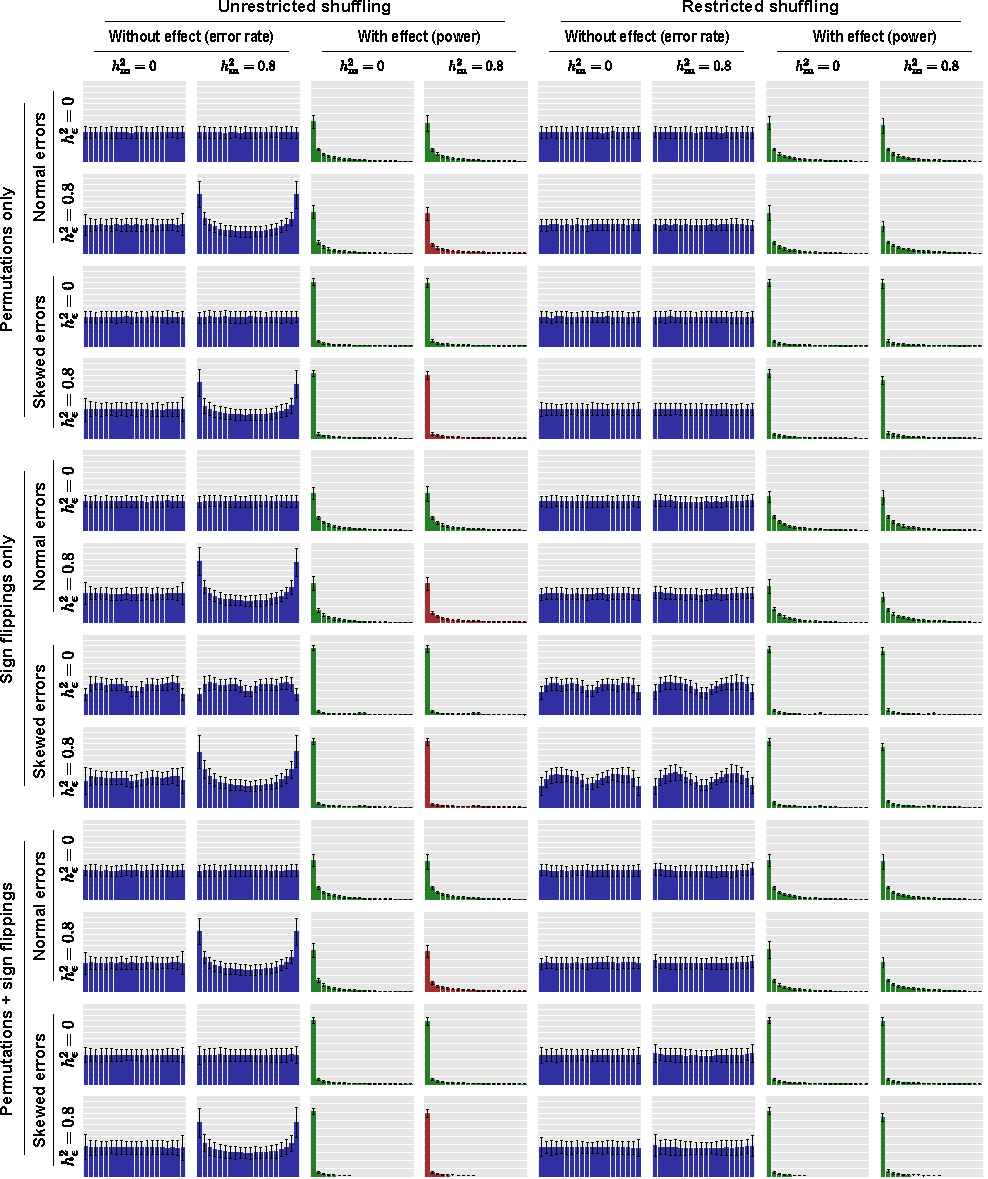
\includegraphics[width=\textwidth]{figures/errorrates.pdf}
\label{fig:errorrates_noref}
\end{figure}

\begin{figure}[!tp]
\centering
\hspace*{-5mm}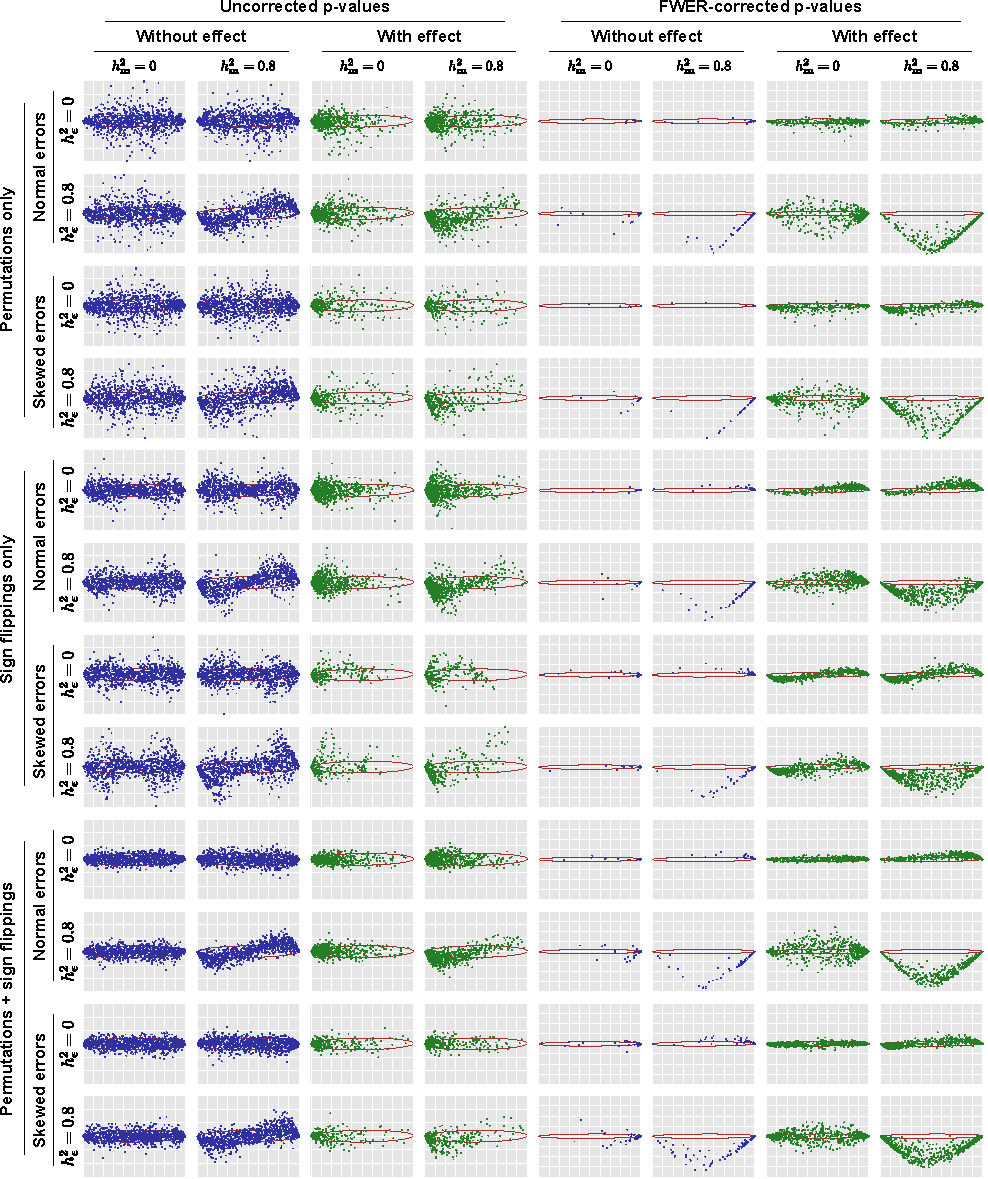
\includegraphics[width=\textwidth]{figures/bland_altman.pdf}
\label{fig:bland_altman_noref}
\end{figure}

\subsection{Power}

For the nine synthetic datasets, a slight, yet consistent loss of power was observed when using the proposed restricted shuffling strategy, compared to the results using unrestricted shuffling when the last was, in fact, possible. These results are shown in Table~\ref{tab:hamming}. The loss appears to be larger for the datasets with more involved dependence structures (e.g., dataset \textsc{d}), or when restrictions on permutations are imposed at higher levels (e.g., dataset \textsc{e}), or on sign flippings at lower levels (e.g., datasets \textsc{f} and \textsc{g}). Even so, this is not quite as conspicuous with samples that are just modestly larger (e.g., \textsc{a} and \textsc{b}), or much larger (e.g., datasets \textsc{h} and \textsc{i}, that use the data structure from the \textsc{hcp}).

\begin{table}[!tp]
\caption[Relationship between Hamming distance and power.]{Relationship between the average Hamming distance across shufflings and the observed power ($\pm$ standard deviation). In general, larger reductions in the Hamming distance when using restricted permutations (\textsc{ee}) caused more noticeable losses in power (see also Figure~\ref{fig:hamming}). The loss did not correlate with the Hamming distance when using sign flippings only (\textsc{ise}) or permutations with sign flippings (\textsc{ee+ise}). In these cases, the power changes were generally minimal.}
\begin{center}
{\small
\begin{tabular}{@{}lr@{\hspace{3pt}}c@{\hspace{3pt}}lr@{\hspace{3pt}}c@{\hspace{3pt}}lr@{\hspace{3pt}}c@{\hspace{3pt}}lr@{\hspace{3pt}}c@{\hspace{3pt}}l@{}}
\toprule
{} & \multicolumn{6}{c}{Unrestricted shuffling} & \multicolumn{6}{c}{Restricted shuffling} \\
\cmidrule(lr){2-7} \cmidrule(l){8-13}
{} & \multicolumn{3}{c}{Hamming} & \multicolumn{3}{c}{Power} & \multicolumn{3}{c}{Hamming} & \multicolumn{3}{c}{Power}\\
Set & \multicolumn{3}{c}{distance} & \multicolumn{3}{c}{(\%)} & \multicolumn{3}{c}{distance} & \multicolumn{3}{c}{(\%)}\\
\midrule
\multicolumn{13}{l}{\emph{Permutations only:}}\\
\textsc{a} & 34.929 & $\pm$ & 0.051 & 49.17 & $\pm$ & 7.18 & 33.956 & $\pm$ & 0.123 & 47.97 & $\pm$ & 7.22 \\
\textsc{b} & 25.945 & $\pm$ & 0.052 & 48.45 & $\pm$ & 7.77 & 24.956 & $\pm$ & 0.104 & 46.68 & $\pm$ & 7.57 \\
\textsc{c} & 9.980 & $\pm$ & 0.041 & 46.52 & $\pm$ & 10.92 & 9.981 & $\pm$ & 0.044 & 46.57 & $\pm$ & 10.73 \\
\textsc{d} & 16.965 & $\pm$ & 0.044 & 48.01 & $\pm$ & 10.93 & 11.003 & $\pm$ & 0.122 & 32.48 & $\pm$ & 8.48 \\
\textsc{e} & 13.973 & $\pm$ & 0.048 & 47.57 & $\pm$ & 10.23 & 9.991 & $\pm$ & 0.106 & 34.58 & $\pm$ & 8.80 \\
\textsc{f} & 13.867 & $\pm$ & 0.084 & 45.16 & $\pm$ & 10.11 & 12.000 & $\pm$ & 0.000 & 38.14 & $\pm$ & 8.69 \\
\textsc{g} & 13.972 & $\pm$ & 0.047 & 47.46 & $\pm$ & 10.18 & 13.975 & $\pm$ & 0.066 & 46.93 & $\pm$ & 10.21 \\
\textsc{h} & 515.996 & $\pm$ & 0.042 & 49.59 & $\pm$ & 2.37 & 496.000 & $\pm$ & 0.307 & 48.41 & $\pm$ & 2.16 \\
\textsc{i} & 515.994 & $\pm$ & 0.043 & 49.56 & $\pm$ & 2.25 & 496.063 & $\pm$ & 0.326 & 48.45 & $\pm$ & 2.23 \\
\midrule
\multicolumn{13}{l}{\emph{Sign flippings only:}}\\
\textsc{a} & 17.959 & $\pm$ & 0.131 & 48.13 & $\pm$ & 6.81 & 18.000 & $\pm$ & 0.000 & 44.74 & $\pm$ & 6.28\\
\textsc{b} & 13.476 & $\pm$ & 0.109 & 47.23 & $\pm$ & 7.66 & 13.500 & $\pm$ & 0.000 & 44.06 & $\pm$ & 7.17\\
\textsc{c} & 5.495 & $\pm$ & 0.062 & 44.16 & $\pm$ & 10.27 & 5.489 & $\pm$ & 0.069 & 44.20 & $\pm$ & 10.07\\
\textsc{d} & 8.715 & $\pm$ & 0.375 & 42.83 & $\pm$ & 10.97 & 9.000 & $\pm$ & 0.000 & 38.59 & $\pm$ & 8.75\\
\textsc{e} & 7.492 & $\pm$ & 0.076 & 45.04 & $\pm$ & 9.05 & 7.479 & $\pm$ & 0.074 & 45.00 & $\pm$ & 9.29\\
\textsc{f} & 7.215 & $\pm$ & 0.332 & 41.81 & $\pm$ & 10.35 & 7.500 & $\pm$ & 0.000 & 38.45 & $\pm$ & 7.99\\
\textsc{g} & 7.292 & $\pm$ & 0.366 & 42.06 & $\pm$ & 10.22 & 7.500 & $\pm$ & 0.000 & 38.45 & $\pm$ & 7.99\\
\textsc{h} & 258.528 & $\pm$ & 0.478 & 49.48 & $\pm$ & 2.23 & 258.440 & $\pm$ & 0.900 & 49.36 & $\pm$ & 2.34\\
\textsc{i} & 258.542 & $\pm$ & 0.505 & 49.59 & $\pm$ & 2.33 & 258.525 & $\pm$ & 0.761 & 49.41 & $\pm$ & 2.33\\
\midrule
\multicolumn{13}{l}{\emph{Permutations with sign flippings:}}\\
\textsc{a} & 35.432 & $\pm$ & 0.042 & 50.07 & $\pm$ & 7.19 & 34.913 & $\pm$ & 0.095 & 50.00 & $\pm$ & 7.19\\
\textsc{b} & 26.449 & $\pm$ & 0.040 & 49.72 & $\pm$ & 7.74 & 25.914 & $\pm$ & 0.092 & 49.24 & $\pm$ & 7.56\\
\textsc{c} & 10.483 & $\pm$ & 0.041 & 50.30 & $\pm$ & 10.97 & 10.471 & $\pm$ & 0.033 & 50.32 & $\pm$ & 10.91\\
\textsc{d} & 17.465 & $\pm$ & 0.041 & 49.94 & $\pm$ & 11.11 & 14.450 & $\pm$ & 0.137 & 46.29 & $\pm$ & 10.55\\
\textsc{e} & 14.471 & $\pm$ & 0.039 & 49.87 & $\pm$ & 10.19 & 12.452 & $\pm$ & 0.088 & 48.81 & $\pm$ & 10.11\\
\textsc{f} & 14.472 & $\pm$ & 0.039 & 49.93 & $\pm$ & 10.18 & 13.470 & $\pm$ & 0.085 & 47.79 & $\pm$ & 9.85\\
\textsc{g} & 14.474 & $\pm$ & 0.035 & 49.95 & $\pm$ & 10.15 & 14.456 & $\pm$ & 0.055 & 49.05 & $\pm$ & 10.16\\
\textsc{h} & 516.480 & $\pm$ & 0.036 & 49.68 & $\pm$ & 2.26 & 505.953 & $\pm$ & 0.569 & 49.65 & $\pm$ & 2.31\\
\textsc{i} & 516.481 & $\pm$ & 0.038 & 49.61 & $\pm$ & 2.32 & 506.072 & $\pm$ & 0.570 & 49.69 & $\pm$ & 2.25\\
\bottomrule
\end{tabular}}
\end{center}
\label{tab:hamming}
\end{table}

With exchangeable errors, in which only permutations are performed, power reductions were more noticeable for some datasets and related well to how the data could be disarranged at each permutation, as quantified by the average Hamming distance across the permutations that were performed. This is shown in Table~\ref{tab:hamming}, and also visually in Figure \ref{fig:hamming}. With independent and symmetric errors, in which only sign flippings are performed, the power losses were considerably smaller, and unrelated to the Hamming distance. In the same manner, permutations combined with sign flippings showed power changes that were minimal, and unrelated to the Hamming distance. Moreover, in these cases the resulting power was, for all datasets, higher than for just permutations or just sign flippings.

\begin{figure}[!tp]
\centering
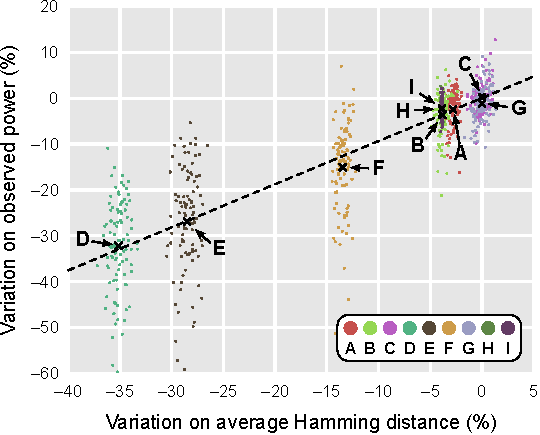
\includegraphics{figures/hamming.pdf}
\caption[Relationship between Hamming distance and power.]{Changes in power related well to the average Hamming distance across permutations for the nine simulated datasets \textsc{a}--\textsc{i} (see also Table~\ref{tab:hamming}). When all dots are considered, $R^2 = 0.7557$ for a linear fit (dashed line); when only the centres of mass for each dataset (marked with ``$\times$'' and indicated with arrows) are considered, $R^2 = 0.9902$.}
\label{fig:hamming}
\end{figure}

Table~\ref{tab:hamming} and Figure~\ref{fig:hamming} show a considerable dispersion of the observed power around the average. In the simulations, this dispersion can be reduced by one order of magnitude approximately just by using the same data and design for all repetitions, varying only the set of shufflings that are performed. Although this reduced dispersion would reflect more accurately the actual variation that different shufflings would cause on a given real experiment, the average power would be dependent on the exact, but random values used for the simulations, and would not be appropriate for the investigation performed here. The magnitude of variations on power as shown does not translate to actual experiments and should not be interpreted as such.

\subsection{Real data}

Summary statistics for height, weight, \textsc{bmi}, global cortical surface area, and global average thickness for the analysed \textsc{hcp} sample are shown in Table~\ref{tab:heritabilities}. The same Table also shows that, consistently with the literature, all these quantities are highly and significantly heritable, even when a conservative surrogate for common environment is included in the model. In fact, the estimated common environment fraction of the variance ($c^2$) was zero for all traits except for height. When the shared environment term is removed from the model, the estimated heritability for height increases to 0.8771 (standard error: 0.0244, $2D_{\text{LL}}$ = 146.9, p-value: 4.1 $\cdot$ 10$^{-34}$).

\begin{table}[!tp]
\caption[Heritabilities for the indices of body size and for global cortical surface area and thickness.]{Heritabilities ($h^2$) for the indices of body size and for global cortical surface area and global average thickness on the sample of \textsc{hcp} subjects when a surrogate for common enviroment effects ($c^2$) is included in the model. The standard errors (\textsc{se}), the test statistic ($2D_{\text{LL}}$), and the p-values are also shown. Only for height the common environment effect was estimated to be different than zero. All traits being highly heritable implies that permutation for analysis of their relationship must take the dependence structure into account.}
{\small
\begin{center}
\hspace*{-3mm}\begin{tabular}{@{}lllrlllrl@{}}
\toprule
{} & \multicolumn{4}{c}{Additive genetic} & \multicolumn{4}{c}{Common environment}\\
\cmidrule(lr){2-5} \cmidrule(l){6-9}
Trait & $h^2$ & \textsc{se} & $2D_{\text{LL}}$ & p-value & $c^2$ & \textsc{se} & $2D_{\text{LL}}$ & p-value\\
\midrule
Height       & 0.7346 & 0.1035 & 35.4  & $1.3 \cdot 10^{-9}$  & 0.1409 & 0.0990 & 1.9 & $8.7 \cdot 10^{-2}$\\
Weight       & 0.7248 & 0.0580 & 61.1  & $2.8 \cdot 10^{-15}$ & 0.0000 & -- & -- & --\\
\textsc{bmi} & 0.7390 & 0.0572 & 62.1  & $1.6 \cdot 10^{-15}$ & 0.0000 & -- & -- & --\\
Area         & 0.8697 & 0.0274 & 125.3 & $2.2 \cdot 10^{-29}$ & 0.0000 & -- & -- & --\\
Thickness    & 0.8961 & 0.0232 & 125.5 & $1.9 \cdot 10^{-29}$ & 0.0000 & -- & -- & --\\
\bottomrule   
\end{tabular}
\end{center}}
\label{tab:heritabilities}
\end{table}

Permuting the data freely to test the hypotheses of correlation between thickness or area and indices of body size, therefore not respecting the structure of the sibships, allowed the identification of a few seemingly significant associations, even after \textsc{fwer} correction across the whole brain, and considering that both positive and negative tests were being performed. These regions, shown in Figure~\ref{fig:realdata}, are (1) left anterior cingulate for a positive correlation between height and cortical surface area, (2) right orbitofrontal medial cortex for a positive correlation between thickness and \textsc{bmi}, (3), right temporal pole, at the confluence of the inferior temporal gyrus, for a negative correlation between thickness and body weight, and (4) right inferior temporal gyrus for a negative correlation between thickness and height. All these regions are very small, two of them comprising just one vertex at the resolution of the surfaces. However, using the proposed multi-level permutation strategy, in which shufflings only happen within siblings of the same type, and in which families with identical structure are allowed to be permuted as a whole, therefore respecting the kinship structure, all these findings became no longer significant. Table~\ref{tab:minfwep} shows the minimum (most significant) p-value throughout the brain for both unrestricted and restricted permutation.

\begin{figure}[!p]
\centering
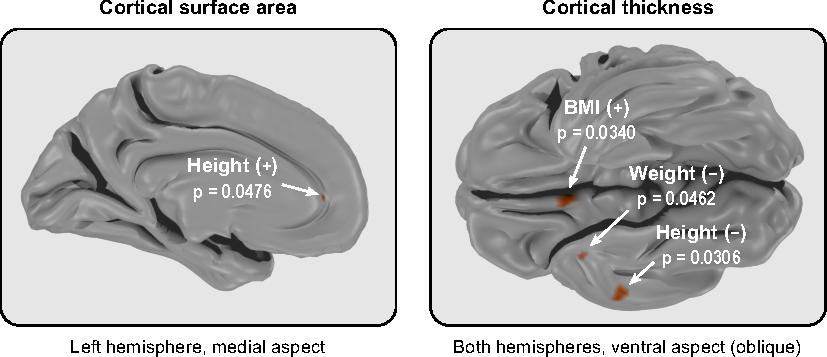
\includegraphics{figures/realdata.pdf}
\caption[Maps showing significant correlations (false positives) of height, weight, and \textsc{bmi} with cortical surface area and thickness.]{Maps showing the locations of the peaks of significance, for positive ($+$) and negative ($-$) correlations of height, weight, and \textsc{bmi} with cortical surface area and thickness. For conciseness, and given their lack of overlap, the original maps for thickness were thresholded at 0.05 and added together, allowing the regions to be displayed in the same figure. Even after using \textsc{fwer}-correction across the brain and contrasts, the unrestricted shuffling identified seemingly significant regions; these regions were not found significant using the restricted permutations that respect the family structure in the \textsc{hcp} sample. Provided that these traits are highly non-independent between subjects (i.e., heritable) this suggests that these results, produced with simple, unrestricted permutation, are in fact \textbf{false positives} (the peaks of significance for both restricted and unrestricted are listed in Table~\ref{tab:minfwep}).}
\label{fig:realdata}
\end{figure}

\begin{table}[!p]
\caption[Peak significance levels for each of the correlations between height, weight and \textsc{bmi}, and cortical thickness and local cortical surface area (false positives).]{Peak significance levels for each of the correlations between height, weight and \textsc{bmi}, and cortical thickness and local cortical surface area. The p-values below $\alpha = 0.05$ are marked in \textbf{bold}; all values are corrected controlling the familywise-error rate (\textsc{fwer}) across the whole brain and across both positive and negative correlations. Permuting the data freely, therefore violating exchangeability, identified seemingly significant associations. However, using the proposed permutation strategy that respects the data structure, these findings disappear, suggesting that these significant results are, in fact, \textbf{false positives}. See also Figure~\ref{fig:realdata} in the main text.}
{\small
\begin{center}
\begin{tabular}{@{}lcccccccc@{}}
\toprule
{} & \multicolumn{4}{c}{Cortical surface area} & \multicolumn{4}{c}{Cortical thickness}\\
\cmidrule(rl){2-5} \cmidrule(l){6-9}
Trait & \multicolumn{2}{c}{Unrestricted} & \multicolumn{2}{c}{Restricted} & \multicolumn{2}{c}{Unrestricted} & \multicolumn{2}{c}{Restricted}\\
\cmidrule(rl){2-3} \cmidrule(rl){4-5} \cmidrule(rl){6-7} \cmidrule(l){8-9}
{} & Left & Right & Left & Right & Left & Right & Left & Right \\
\midrule
\multicolumn{9}{l}{\emph{Positive correlation:}}\\
Height & \textbf{0.0476} & 0.2178 & 0.1530 & 0.4398 & 0.4168 & 0.0734 & 0.6438 & 0.1694 \\
Weight & 0.9524 & 0.7448 & 0.9724 & 0.8346 & 0.2348 & 0.1706 & 0.3118 & 0.2376 \\
\textsc{bmi} & 1.0000 & 0.9368 & 1.0000 & 0.9586 & 0.0950 & \textbf{0.0340} & 0.1376 & 0.0522 \\
\midrule
\multicolumn{9}{l}{\emph{Negative correlation:}}\\
Height & 0.9674 & 0.9936 & 0.9944 & 0.9996 & 0.2206 & \textbf{0.0306} & 0.4204 & 0.0788\\
Weight & 0.9960 & 0.9908 & 0.9992 & 0.9978 & 0.1246 & \textbf{0.0462} & 0.1860 & 0.0810\\
\textsc{bmi} & 0.8002 & 0.9848 & 0.8644 & 0.9926 & 0.4492 & 0.2674 & 0.5620 & 0.3588 \\
\bottomrule
\end{tabular}
\end{center}}
\label{tab:minfwep}
\end{table}

\section{Discussion}

\subsection{Error rates and power}

The proposed multi-level shuffling strategy controlled the false positive rate at the nominal level in all configurations evaluated. With the only exception of sign flippings in the presence of skewed errors, which clearly violates assumptions, the empirical distribution of p-values was uniform, as desired, whenever shufflings respected the dependence structure present in the data; ignoring the dependence resulted in inflated error rates, rendering the test invalid. Dependencies in both data and model are present, for example, whenever an association between two heritable variables are investigated in a genetically informative sample, such as sibships (or even general pedigrees) as in the \textsc{hcp} case shown.

The guaranteed validity and exactness of p-values came, however, at the price of a small, yet noticeable and consistent reduction in power, that related to the complexity of the dependence structure and the ensuing restrictions on exchangeability. This can be understood by noting that the restricted permutation strategy does not disarrange the data as much as the unrestricted shuffling, with the consequence that the statistics computed after permuting the data may not be as distant from the statistic computed from the unpermuted data. With sign flippings, the power losses were smaller, and unrelated to the Hamming distance, presumably because even changes seemingly small, such as a single sign swap, can cause large perturbations on the shuffled data, sufficient to minimise reductions on sensitivity. Permutations combined with sign flippings showed minimal power changes that were also unrelated to the average Hamming distance, and with losses that were smaller than for just permutations or just sign flippings, suggesting that when both \textsc{ee} and \textsc{ise} are valid for a given model, permutations with sign flippings can allow maximum efficiency.\footnote{It should be noted, however, that explicitly selecting permutations that maximise the amount of disarrangement applied to the data, i.e., performing only those with highest Hamming distance, cause the error rates not to be controlled; conversely, a selection of only those that cause less shuffling cause the test to become conservative (results not shown).}

Although the diminished sensitivity could suggest that the multi-level permutation strategy would be ``conservative'' this is not the case, as can be attested by the exact control over error rates. This apparent incongruity can be understood through the Bland--Altman plots in Figure \ref{fig:bland_altman}, that show that the differences in uncorrected p-values between both strategies is largely outside the margins of the confidence interval in both directions, suggesting that, under the null, variations in p-values can go in any direction when the strategies are compared. Nonetheless, in the presence of signal, or when the p-values are corrected for multiple testing using the distribution of the largest statistic across variables (such as voxels), the p-values for the restricted strategy tend to be stochastically larger than those for the free shuffling.

The restrictions imposed on the possible rearrangements that can be performed, with the consequent reduction in the number of possible permutations, as well as the lessened sensitivity, could be seen as negative, but in fact, such restrictions establish a set of rules under which permutation inference can be performed in settings where otherwise it would not possible without appealing to often untenable assumptions, or that would not be possible at all. Simple permutation, if performed, would create data that could be impossible to be observed in practice, and thus, that should not be used to construct the reference distribution to test the hypotheses of interest. Moreover, the stronger the dependency is between observations, the fewer genuinely independent pieces of information are available to test a given hypothesis; in this scenario, smaller power does not appear unexpected.

\subsection{Body size and cortical morphology}

Height, weight, and \textsc{bmi} are known to be highly heritable in general, and were so for the \textsc{hcp} sample. Likewise, the heritability for global cortical surface area and average thickness are known to be heritable, and were found as such in the sample analysed. All these traits remained highly heritable even when a potential confound --- a surrogate for household and maternal effects --- was included. Even if estimated heritability were reduced, common effects would still cause the observations not to be independent. The fact that for all these traits there is a strong dependence between the observations implies that a permutation test that ignores the relationship between observations would not be valid, by violating the exchangeability assumption.

Indeed, the test that shuffled the data freely identified a few positive and negative localised significant associations between indices of body size and cortical area and thickness, even after \textsc{fwer} correction considering all tests in both hemispheres and the fact that positive and negative hypotheses were being tested. None of these areas were found to be significant if the test used only permutations that respected the structure present in the data, in the multi-level fashion, suggesting that these findings are likely false positives. None of the regions implicated were reported in previous studies that investigated relationships between indices of body size and cortical morphology \citep{Pannacciulli2006, Raji2010, Ho2010, Ho2011, Smucny2012, Curran2013, Marques-Iturria2013, Melka2013, Bond2014} that we could identify. It should be conceded, however, that not all these studies used the same methods, with some having analysed gray matter volumes in voxel-based representations of the brain, and some, despite using surface-based methods, performed analyses in macroscopic regions, as opposed to at each point in the cortical mesh. Still, as the simulations demonstrated, the violation of the exchangeability assumption makes the free permutation prone to inflated amounts of error type \textsc{i} if the observations are not independent, and the absence of similar findings from the literature supports the likelihood that these seemingly significant findings are not genuine, being instead false positives.\footnote{We have run a side analysis (not shown) in which we treated \textsc{dz} pairs as ordinary siblings, i.e., using the tree shown in Figure~\ref{fig:treeHCP_dz2sib} instead of the one in Figure~\ref{fig:treeHCP_full}, and observed results that are very similar to those reported, that is, nothing significant.}

Another aspect is that, although \textsc{fwer}-correction was applied considering the multiplicity of vertices in the mesh representation of the cortex and the two contrasts (positive and negative), no correction was applied considering that overall six tests were performed (three independent variables versus two dependent variables); \textsc{fwer}-controlling procedures that would take into account the non-independence between these tests are currently not available. Using Bonferroni correction, the results using the free permutation, which are likely false-positives as discussed above, disappear. Since most studies --- and in fact, most of those referenced in the previous paragraph --- investigated only the relationship between one independent versus one dependent variable, for which no such correction is necessary, the results shown emulate well the risk of false positives in similar, real studies.

\subsection{Applications and other considerations}

In addition to the above examples, and most clearly, with a direct application for the \textsc{hcp} data, the multi-level permutation strategy can be considered for repeated measurements designs in which within- and between-subject factors are tested in the same model or contrast, such as for a continuous regressor. A direct comparison of the power observed for datasets \textsc{e}, \textsc{f} and \textsc{g}, using permutations only, shows that even with the same number of subjects, the combination of within-block with whole-block permutation can be more powerful than each of these used in isolation. Moreover, the strategy can also be considered when not all measurements for a given subject are available, as long as compound symmetry within subject remains valid, without the need to exclude entirely the data for subjects as would be the case for whole-block permutation.

As experiments are planned considering strategies for subsequent analyses, the use of permutation tests can be included among the tools available, especially given its simplicity and, as demonstrated here and in a large body of literature, flexibility to accommodate designs and data that can be quite complex. Adequate planning includes ensuring that assumptions for permutation tests are met from the beginning, such as that the random errors of the instrument are stable along time, and do not vary with the values they measure, that the observations if not independent, possess a dependence structure that can be accommodated in a framework as the one shown here, and that observations, if not homogeneous, can be broadly qualified into a few number of variance groups.

Indeed, regarding \textsc{vg}s, the compatibility of these with the blocks ensures the feasibility of permutation tests, but it also allows that the necessary assumptions are reduced to a minimum: instead of requiring that all observations are homoscedastic (strong), the maximum possible amount of heterogeneity of variances that could still permit the shuffling as indicated by the blocks (weaker assumption) can be allowed. In this case, homogeneity would still be there, although not across all and every observation, just the minimal amount necessary so that the experiment can still be analysed. These considerations may not be relevant if the recruiting process, experimental conditions or data collection can guarantee that the same variance is homogeneous, but may be necessary when the data collection or samples are not under direct control of the researcher (e.g., reanalysis of past experiments, or census data).
\cleardoublepage \chapter{Faster permutation inference}
\label{sec:accel}
\setstretch{\lspac}

\section{Introduction}
\label{sec:accel:intro}
\setstretch{\lspac}

Permutation tests allow exact control of error rates, with minimal assumptions. However, permutation tests are computationally intensive. For small, non-imaging datasets, recomputing a model thousands of times is seldom a problem, but for imaging applications, that involve testing at thousands of spatial points (voxels, vertices, faces, edges), large models that involve many subjects, multiple measurements, pointwise (voxelwise) regressors, spatial statistics, as well as other sources of complexity, even with the availability of inexpensive computing power, the same procedure can be prohibitively slow. Strategies to accelerate the process include the use of efficient or optimised code, the use of parallel, multi-threaded, or distributed computing, and the use of graphics processing units (\textsc{gpu}s) \citep[for example applications of the latter, see][]{Eklund2012, Eklund2013, Hernandez2013}. While these methods are attractive for increases in speed, none reduce the amount of tasks that effectively need to be executed, and the improvements in speed happen through more efficient use of resources available, or through the introduction of yet more resources. At a time in which Moore's law \citep{Moore1965} approaches physical limits \citep{Waldrop2016}, alternative methods to expedite computation are expected to gain prominence.

Here we exploit properties of the statistics themselves and their distributions, which could be used to accelerate the evaluation of the test in order to accept or reject the null hypothesis in a fraction of the time that otherwise would be needed with a large number of permutations. The main tenet of these approaches is to obtain a reduction of the number of actual computations that need to be performed, such that acceleration can be obtained in addition to, or irrespective of, generic improvements of software or hardware. In particular, we discuss the following approaches: ({i}) performing a small number of shufflings (with no other change from the usual case of permutation tests); ({ii}) estimation of the p-value as a parameter of a negative binomial distribution; ({iii}) fitting of a generalised Pareto distribution to the tail of the empirical permutation distribution; ({iv}) computing the p-values based on the expected moments of the empirical distribution, approximated from a gamma distribution; ({v}) direct fitting of a gamma distribution to the empirical distribution; and ({vi}) shuffling of a reduced number of points (e.g., voxels), with completion of the remainder using low rank matrix theory. Details of each are provided in the \href{sec:accel:theory}{Theory} section.

Very few of such acceleration strategies have been investigated or used in brain imaging. The tail approximation was considered by \citet{Ge2012} for an imaging genetics application in which, due to the sheer volume of data, conventional permutation tests were not considered feasible. A variant of many possible algorithms for low rank matrix completion was proposed by \citet{Hinrichs2013}. The fitting of a gamma distribution without the need for permutations was proposed recently for a range of statistics by \citet{Minas2014}. For inference for support-vector machine problems, \citet{Gaonkar2012} suggested an analytical approximation to the permutation distribution of each component of the hyperplane that separates classes. Here we aim to study, evaluate, and in some cases propose, solutions that can accelerate permutation tests for the general linear model (\textsc{glm}), considering aspects that are specially relevant to imaging, such as the multiplicity of tests and the use of spatial statistics. In particular, we make the following main contributions: (\textsc{i}) show how a connection between Pillai's trace and the popular univariate $t$ statistic allows the direct computation of the p-values from the permutation distribution, even without performing actual permutations, (\textsc{ii}) use the moments of the empirical permutation distribution for the fit of a gamma distribution, and (\textsc{iii}) propose a novel low rank matrix completion algorithm, writing the test statistic as the product of two matrices that can be sampled sparsely, and allowing exact recovery of what otherwise would be an approximation.

In the \href{sec:accel:theory}{Theory} section we begin by briefly reviewing the uni- and multivariate \textsc{glm}, their assessment using permutation tests, and introduce the notation used throughout the chapter. The six different acceleration strategies are then presented in sequence, followed by certain aspects related to spatial statistics and multiple testing correction in the context of these methods. In the \href{sec:accel:evaluation}{Evaluation} and \href{sec:accel:results}{Results} sections we assess the performance of these different methods on both synthetic and real data. In the \href{sec:accel:discussion}{Discussion} we provide recommendations for general circumstances. A summary of the acceleration strategies is provided in Table~\ref{tab:summary}. Figure \ref{fig:curvefits} illustrates four of them.

\begin{table}[!b]
\caption[Overview of various strategies that can be considered to accelerate permutation tests.]{\emph{(page \pageref{tab:summary_noref})} Overview of various strategies that can be considered to accelerate permutation tests. \textsc{cmv}: Classical multivariate test (such as \textsc{mancova}); \textsc{npc}: Non-Parametric Combination; see \citet{Winkler2016_npc} for details. Although the tail and gamma approximations can be considered for essentially any permutation distribution (the latter particularly for unimodal distributions), the \href{sec:accel:results}{Results} showed that the fit performs better for the distribution of the extremum statistic, as used for familywise error rate (\textsc{fwer}) correction. The negative binomial can be used for \textsc{npc}, although unlikely with any acceleration benefit. For low rank matrix completion, many algorithmic variants can be considered, and the complexity needed for \textsc{cmv} and \textsc{npc} may offset speed benefits; for this method, spatial statistics can be computed from the completed non-spatial (pointwise) statistics, although a direct computation, in a similar way as for the pointwise, would require a different algorithm with results that would likely not be exact. See main text for details on this and on all other methods.\par}
\label{tab:summary}
\end{table}

\begin{sidewaystable}
\vspace*{5mm}
{\footnotesize
\begin{center}
\begin{tabular}{
@{}m{2.1cm}<{\raggedright}@{\hspace{3mm}}
m{8.0cm}<{\raggedright}@{\hspace{6mm}}
c@{\hspace{3mm}}
c@{\hspace{3mm}}
c@{\hspace{3mm}}
c@{\hspace{6mm}}
c@{\hspace{3mm}}
c@{\hspace{3mm}}
c@{\hspace{3mm}}
c@{\hspace{6mm}}
c@{\hspace{3mm}}
c@{\hspace{3mm}}
c@{\hspace{3mm}}
c@{}}
\toprule
{} & {} & \multicolumn{4}{c}{Univariate} & \multicolumn{4}{c}{\textsc{cmv}} & \multicolumn{4}{c}{\textsc{npc}}\\
\cmidrule(lr){3-6} \cmidrule(lr){7-10} \cmidrule(l){11-14}
{Method} & Brief description 
& \multicolumn{2}{c}{Pointwise} & \multicolumn{2}{c}{Spatial} 
& \multicolumn{2}{c}{Pointwise} & \multicolumn{2}{c}{Spatial} 
& \multicolumn{2}{c}{Pointwise} & \multicolumn{2}{c}{Spatial}\\
\cmidrule(lr){3-4} \cmidrule(lr){5-6}
\cmidrule(lr){7-8} \cmidrule(lr){9-10}
\cmidrule(lr){11-12} \cmidrule(l){13-14}
{} & {} 
& unc.\ & corr.\ 
& unc.\ & corr.\ 
& unc.\ & corr.\ 
& unc.\ & corr.\ 
& unc.\ & corr.\ 
& unc.\ & corr.\ \\
\midrule
Few per\-mu\-ta\-tions &
Compute the p-values using just a few permutations, e.g., less than a thousand. &
{\color{blue}\ding{'63}} & {\color{blue}\ding{'63}} &
{\color{blue}\ding{'63}} & {\color{blue}\ding{'63}} &
{\color{blue}\ding{'63}} & {\color{blue}\ding{'63}} &
{\color{blue}\ding{'63}} & {\color{blue}\ding{'63}} &
{\color{blue}\ding{'63}} & {\color{blue}\ding{'63}} &
{\color{blue}\ding{'63}} & {\color{blue}\ding{'63}}\\
\midrule
Negative binomial &
Run for each voxel as many permutations as needed until a predefined number of exceedances is found. Then divide this number of by the number of permutations. &
{\color{blue}\ding{'63}} & {\color{darkgreen}$\bullet$} &
{\color{red}\ding{'67}}  & {\color{darkgreen}$\bullet$} &
{\color{blue}\ding{'63}} & {\color{darkgreen}$\bullet$} &
{\color{red}\ding{'67}}  & {\color{darkgreen}$\bullet$} &
{\color{darkgreen}$\bullet$} & {\color{darkgreen}$\bullet$} &
{\color{red}\ding{'67}}  & {\color{darkgreen}$\bullet$}\\
\midrule
Tail approximation &
Run a small number of permutations and, for the p-values below a certain threshold (e.g., 0.10), fit a generalised Pareto distribution, modelling the tail of the permutation distribution. &
{\color{darkgreen}$\bullet$} & {\color{blue}\ding{'63}} &
{\color{darkgreen}$\bullet$} & {\color{blue}\ding{'63}} &
{\color{darkgreen}$\bullet$} & {\color{blue}\ding{'63}} &
{\color{darkgreen}$\bullet$} & {\color{blue}\ding{'63}} &
{\color{darkgreen}$\bullet$} & {\color{blue}\ding{'63}} &
{\color{darkgreen}$\bullet$} & {\color{blue}\ding{'63}}\\
\midrule
No permutation &
For statistics that can be written as $\text{trace}(\mathbf{A}\mathbf{W})$, where $\mathbf{A}=\mathbf{X}\mathbf{X}^{+}$, $\mathbf{W}=\mathbf{U}\mathbf{U}'$, and $\mathbf{U}\mathbf{S}\mathbf{V}'=\text{svd}(\mathbf{R}_{\mathbf{Z}}\mathbf{Y})$, compute analytically the moments of the permutation distribution, then fit a gamma distribution. &
{\color{blue}\ding{'63}} & {\color{red}\ding{'67}} &
{\color{red}\ding{'67}}  & {\color{red}\ding{'67}} &
{\color{blue}\ding{'63}} & {\color{red}\ding{'67}} &
{\color{red}\ding{'67}}  & {\color{red}\ding{'67}} &
{\color{red}\ding{'67}}  & {\color{red}\ding{'67}} &
{\color{red}\ding{'67}}  & {\color{red}\ding{'67}}\\
\midrule
Gamma approximation &
Run a small number of permutations, compute empirically the moments of the permutation distribution, then fit a gamma distribution. &
{\color{darkgreen}$\bullet$} & {\color{blue}\ding{'63}} &
{\color{darkgreen}$\bullet$} & {\color{blue}\ding{'63}} &
{\color{darkgreen}$\bullet$} & {\color{blue}\ding{'63}} &
{\color{darkgreen}$\bullet$} & {\color{blue}\ding{'63}} &
{\color{darkgreen}$\bullet$} & {\color{blue}\ding{'63}} &
{\color{darkgreen}$\bullet$} & {\color{blue}\ding{'63}}\\
\midrule
Low rank matrix completion &
Run a certain number of permutations, define ortho\-normal bases for matrices that are linear functions of the data and from which the statistic can be obtained; continue permuting a random subset of tests, filling the missing ones via projection to these bases. &
{\color{blue}\ding{'63}} & {\color{blue}\ding{'63}} &
{\color{darkgreen}$\bullet$} & {\color{darkgreen}$\bullet$} &
{\color{darkgreen}$\bullet$} & {\color{darkgreen}$\bullet$} &
{\color{darkgreen}$\bullet$} & {\color{darkgreen}$\bullet$} &
{\color{darkgreen}$\bullet$} & {\color{darkgreen}$\bullet$} &
{\color{darkgreen}$\bullet$} & {\color{darkgreen}$\bullet$}\\
\bottomrule   
\vspace*{.5mm}
\end{tabular}
\begin{tabular}{l@{\hspace{10mm}}l@{\hspace{10mm}}l}
{\color{blue}\ding{'63}} Can be used.&
{\color{darkgreen}$\bullet$} Can be used, although there are particularities (see main text).&
{\color{red}\ding{'67}} Cannot be used.\\
\end{tabular}
\end{center}}
\label{tab:summary_noref}
\end{sidewaystable}

\begin{figure}[!tp]
\begin{center}
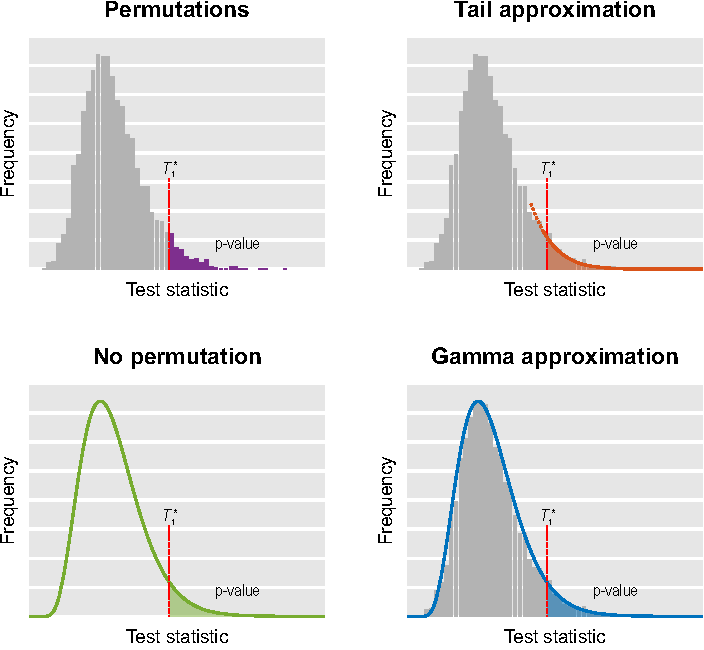
\includegraphics{figures/curvefits.pdf}
\end{center}
\caption[Illustration of some of the acceleration strategies.]{With permutations (i.e., any number of rearrangements, the use of the negative binomial distribution, or the low rank matrix completion), the p-value is the fraction of the test statistics obtained after permuting that are higher than in the unpermuted $T \equiv T_1^*$. In the tail approximation, the tail of the permutation distribution is subjected to the fit of a generalised Pareto distribution (\textsc{gpd}), from which the p-values are computed. In the method in which no permutations are performed, the first three moments of the permutation distribution are computed from data and model, and to these which a gamma distribution (Pearson type \textsc{iii}) can be fitted, and from which the p-values are computed. In the gamma approximation, the moments of the empirical permutation distribution are used to the fit of the gamma distribution. The figure is merely illustrative: the actual fit uses the cumulative distribution function, such that histograms are not constructed in practice, hence the fit does not depend on binning.}
\label{fig:curvefits}
\end{figure}

\section{Theory}
\label{sec:accel:theory}

\subsection{Notation and general aspects}
\label{sec:accel:notation}

At each spatial point of an image representation of the brain, consider a general linear model (\textsc{glm}) \citep{Scheffe1959, Searle1971} expressed as:

\begin{equation}
\mathbf{Y} =  \mathbf{M} \boldsymbol{\psi} + \boldsymbol{\epsilon}
\label{eqn:glmfull}
\end{equation}

\noindent
where $\mathbf{Y}$ is the $N \times K$ matrix of observed data, with $N$ observations of $K$ distinct (possibly non-independent) variables, $\mathbf{M}$ is the full-rank $N \times R$ design matrix of explanatory variables (i.e., effects of interest and possibly nuisance effects), $\boldsymbol{\psi}$ is the $R \times K$ matrix of regression coefficients, and $\boldsymbol{\epsilon}$ is the $N \times K$ matrix of random errors. Estimates for the regression coefficients can be computed as $\boldsymbol{\hat{\psi}} = \mathbf{M}^{+}\mathbf{Y}$, where the superscript ($^{+}$) denotes a generalised inverse. One is generally interested in testing the null hypothesis that a contrast of regression coefficients is equal to zero, i.e., $\mathcal{H}_{0} : \mathbf{C}'\boldsymbol{\psi}\mathbf{D} = \boldsymbol{0}$, where $\mathbf{C}$ is an $R \times S$ full-rank matrix of $S$ contrasts of coefficients on the regressors encoded in $\mathbf{M}$, $1 \leqslant S \leqslant R$ and $\mathbf{D}$ is a $K \times Q$ full-rank matrix of $Q$ contrasts of coefficients on the dependent, response variables in $\mathbf{Y}$, $1 \leqslant Q \leqslant K$; if $K=1$ or $Q=1$, the model is univariate. Once the hypothesis has been established, $\mathbf{Y}$ can be equivalently redefined as $\mathbf{Y}\mathbf{D}$, such that the contrast $\mathbf{D}$ can be omitted for simplicity, and the null hypothesis stated as $\mathcal{H}_{0} : \mathbf{C}'\boldsymbol{\psi} = \boldsymbol{0}$. Another useful simplification is to consider a transformation of the model into a partitioned one:

\begin{equation}
\mathbf{Y} = \mathbf{X}\boldsymbol{\beta} + \mathbf{Z}\boldsymbol{\gamma} + \boldsymbol{\epsilon}
\label{eqn:glmpart}
\end{equation}

\noindent
where $\mathbf{X}$ is the matrix with regressors of interest, $\mathbf{Z}$ is the matrix with nuisance regressors, and $\boldsymbol{\beta}$ and $\boldsymbol{\gamma}$ are respectively the vectors of regression coefficients. Even though such partitioning is not unique, it can be defined in terms of the contrast $\mathbf{C}$ such that the columns of $\mathbf{X}$ and $\mathbf{Z}$ are orthogonal to each other, and inference on $\boldsymbol{\beta}$ is equivalent to inference on $\mathbf{C}'\boldsymbol{\psi}$ \citep{Beckmann2001, Smith2007, Winkler2014}. A suitable, pivotal test statistic, here generically termed $T$, is computed and its significance assessed through permutations and/or sign flippings of the data, the model, the residuals, or variants of these. We sometimes use the terms \emph{rearrangement} or \emph{shuffling} when the distinction between permutations or sign flippings is not pertinent. The p-value is computed as:

\begin{equation}
p=\frac{1}{J}\sum_{j=1}^J I\left( T_j^{*} \geqslant T \right)
\label{eqn:pvalue}
\end{equation}

\noindent
where $I(\cdot)$ is the indicator function, $T_j^{*}$ is the test statistic observed at the $j$-th shuffling of the data, $J$ is the number of rearrangements performed, of which the first (i.e., $j=1$) is the unpermuted case. We denote the significance level of the test as $\alpha$. In typical cases, $J$ is much smaller than the number of unique possible rearrangements allowed by the design and data, $J^{\text{max}}$. The same procedure can be used with classical multivariate tests (\textsc{cmv}), such as \textsc{manova}/\textsc{mancova} or canonical correlation analysis (\textsc{cca}), as well as with Non-Parametric Combination (\textsc{npc}); details for both the univariate and multivariate \textsc{glm} in the context of imaging are discussed in \citet{Winkler2014, Winkler2016_npc}.

\paragraph{Resampling risk} Two methods may have similar error rates and power, yet fail to agree on which tests should have their null hypotheses rejected or retained. The \emph{resampling risk} is a quantity that represents the probability of taking a different decision regarding the rejection or acceptance of the null hypothesis if the procedure is repeated using the same input data, but different methods \citep{Jockel1984}. Compared to confidence intervals, which can be calculated for p-values derived from permutations through a binomial approximation (see the Section \href{sec:accel:fewperms}{Few permutations}), the resampling risk is a more generic quantity in that it provides information on the chance of reaching a different decision regarding the null hypothesis that is computable for all the different methods, including, for instance, the one in which no permutations are used.

\subsection{Acceleration methods}

Nearly all of the acceleration strategies below can be applied to univariate, uncorrected pointwise tests (``pointwise'' as an umbrella term encompassing voxelwise, vertexwise, facewise, as well as nodewise and edgewise graph theoretical measurements, or any other relevant imaging test). If $Q>1$ or $K>1$, the model is multivariate, and \textsc{cmv} or \textsc{npc} can be considered \citep{Winkler2016_npc}. Some of the methods can also be used with spatial test statistics, and for inferences corrected for the familywise error rate (\textsc{fwer}) using the distribution of the extremum statistic (see below).

\subsubsection{Few permutations}
\label{sec:accel:fewperms}

Conditional on the observed data, if all possible rearrangements are performed, a permutation test is exact in that it yields results that are not based on distributional assumptions or asymptotic approximations, but rather represent the exact probability of rejecting the null hypothesis when it is true. If fewer than all possible rearrangements are performed, the p-value obtained is an estimate of the true and unknown p-value; the test continues to be exact in that the probability of obtaining an estimate $\hat{p}$ less than or equal to the significance level $\alpha$, is $\alpha$ itself, i.e., $P(\hat{p}\leqslant\alpha)=\alpha$, provided that the level is sensibly chosen considering the discreteness of the permutation p-values. Thus, a simple strategy for acceleration consists in running only a small number of permutations. As indicated above, this results in an unbiased (i.e., correct on average) estimate of the p-value, but with higher variance (variability around the true value) than when using a large number of permutations. Confidence intervals around $\hat{p}$ can be computed using one of the various methods for Bernoulli trials, such as those proposed by \citet{Wilson1927}, \citet{Clopper1934} or \citet{Agresti1998} \citep[for a comparative review, see][]{Brown2001}. Whichever is used, fewer permutations imply wider intervals (Table~\ref{tab:fewpermCI}), such that the resampling risk can be expected to increase; in the \href{sec:accel:evaluation}{Evaluation} section we assess this risk for the case of a few permutations, as well as for the other acceleration methods.

\begin{table}[!tp]
\caption[Confidence intervals as a function of the number of permutations.]{Confidence intervals (95\%), computed using the Wilson method, for a p-value $P=0.05$ as a function of the number of permutations ($J$). More permutations narrow the confidence interval.}
\begin{center}
\begin{tabular}{@{}m{25mm}<{\raggedright}m{25mm}<{\raggedright}@{}}
\toprule
Number of permutations & Confidence interval\\
\midrule
40 & 0.0138--0.1650\\
60 & 0.0171--0.1370\\
100 & 0.0215--0.1118\\
200 & 0.0274--0.0896\\
300 & 0.0305--0.0808\\
500 & 0.0341--0.0728\\
1000 & 0.0381--0.0653\\
2000 & 0.0413--0.0604\\
5000 & 0.0443--0.0564\\
10000 & 0.0459--0.0544\\
50000 & 0.0481--0.0519\\
\bottomrule
\end{tabular}
\end{center}
\label{tab:fewpermCI}
\end{table}

\subsubsection{Negative binomial}

If the permutations are performed randomly (as opposed to in some order, such as lexicographic), after a few permutations there may already be sufficient information on whether the null should be rejected, and continuation of the process narrows the confidence interval around $\hat{p}$, although with little chance of changing a decision about the rejection of the null hypothesis if the estimated p-value lies far from the test level $\alpha$. The process can therefore be interrupted after some criterion has been reached. Various such criteria have been proposed \citep{Andrews2000, Davidson2000, Fay2002, Fay2007, Gandy2009, Kim2010, Sandve2011, Gandy2013, Ruxton2013}, and of particular interest is the interruption after a predefined number $n$ of exceedances $T_j^{*} \geqslant T$ has been found. Weaker effects will quickly be exceeded after a few random shufflings, whereas stronger effects require insistence in doing more shufflings until exceedances are found. The ensuing p-value is the estimated parameter of a negative binomial distribution \citep{Haldane1945} as $\hat{p}=(n-1)/(j-1)$, where $j$ is the permutation in which $n$ was reached; this does not include the unpermuted case, and once that is considered, the permutation p-value becomes $\hat{p}=n/j$. This method was proposed by \citet{Besag1991}, and compared to other approaches, it is attractive for its negligible computational overhead, and for bypassing the need that $\alpha$ or any other parameter is defined beforehand. If $n$ has not been reached after a sufficiently large predefined number $J$ of permutations, the process can be interrupted regardless, and the p-value computed as in Equation~\ref{eqn:pvalue}.

\subsubsection{Tail approximation}

The limiting distribution of the maximum of a set of identically distributed random variables converges to one of three well known families of distributions, under a form given by the generalised extreme value distribution (\textsc{gev}) [\citet{Gnedenko1943}; for reviews, see \citet{Leadbetter1983, Davison2015}]. More broadly, however, the tail of the distribution of an arbitrary random variable can be approximated using a generalised Pareto distribution (\textsc{gpd}) \citep{PicklandsIII1975}. For a threshold $u\rightarrow\infty$, the limiting distribution of the quantity $y=T-u$, for $T>u$, is $F(y) = 1-(1-\xi y/\sigma)^{1/\xi}$, defined for $y>0$ and $\xi y/\sigma<1$, with parameters $\xi$ (shape) and $\sigma$ (scale).\footnote{The shape parameter $\xi$ of the \textsc{gpd} corresponds to the shape parameter of the generalised extreme value distribution, whereas the scale parameter $\sigma$ relates to the \textsc{gev} scale $s$ as $\sigma=s-\xi(u-\mu)$, where $\mu$ is the \textsc{gev} location parameter.} Methods to estimate the two parameters of the \textsc{gpd} from the observed permutation statistics include maximum likelihood, the method of moments, or the method of probability-weighted moments; all three have similar estimation efficiency for $-1/2 < \xi < 1/2$, as typical in real world applications \citep{Hosking1987, Knijnenburg2009}. Using the method of moments, the estimators of the scale and shape parameters are $\hat{\sigma} = \bar{y}(\bar{y}^2/s^2+1)/2$ and $\hat{\xi}=(\bar{y}^2/s^2-1)/2$, where $\bar{y}$ and $s^2$ are respectively the sample mean and variance of the values $y$ \citep{Hosking1987}. Goodness of fit can be assessed with the Anderson--Darling test \citep{Anderson1952, Choulakian2001, Knijnenburg2009}.

The algorithm proceeds as follows: a small number of permutations is initially performed, the set of test statistics $T^*_j$ is recorded for each image point, and initial p-values computed as in Equation~\ref{eqn:pvalue}. The voxels with p-values above a loose, liberal significance level (such as twice the chosen $\alpha$) remain unchanged; the others have the tail of their permutation distribution used to estimate the \textsc{gpd} parameters. For these, a reasonable, initial threshold $u$ is the $T^*_j$ that defines the upper quartile of their respective permutation distribution. This threshold is iteratively increased until a good fit of the \textsc{gpd} is found; if a good fit is not found when the permutation distribution has been exhausted, no approximation is made, and the initial p-value is not modified; otherwise, a new p-value is computed using the tail of the \textsc{gpd} fitted for that voxel. For the initial permutation distribution, the unpermuted statistic ($T^*_1$) may or may not be included in the process of tail fitting, and the impact of its inclusion depends on the number of permutations used for the initial distribution, as we show in the \href{sec:accel:results}{Results} section.

\subsubsection{No permutation}

Pillai's trace \citep{Pillai1955} is a suitable statistic that can be considered to test $\mathcal{H}_0$. With the partitioned model, it can be computed as $T=\text{trace}(\tilde{\mathbf{Y}}'\mathbf{H}_{\mathbf{X}}\tilde{\mathbf{Y}}(\tilde{\mathbf{Y}}'\tilde{\mathbf{Y}})^{-1})$, where $\mathbf{H}_\mathbf{X}=\mathbf{X}\mathbf{X}^{+}$, $\tilde{\mathbf{Y}}=\mathbf{R}_{\mathbf{Z}}\mathbf{Y}$, $\mathbf{R}_{\mathbf{Z}}=\mathbf{I}-\mathbf{Z}\mathbf{Z}^{+}$, and $\mathbf{I}$ is the $N \times N$ identity matrix. Alternatively, it can be computed as $T=\text{trace}(\mathbf{H}_\mathbf{X}\mathbf{U}\mathbf{U}')$, where $\mathbf{U}$ is a $N \times K$ matrix containing the $K$ left singular vectors of $\tilde{\mathbf{Y}}$ that have non-zero singular values. To see this, let $\mathbf{H} = (\mathbf{C}'\boldsymbol{\hat{\psi}}\mathbf{D})' \left(\mathbf{C}'(\mathbf{M}'\mathbf{M})^{-1}\mathbf{C} \right)^{-1} (\mathbf{C}'\boldsymbol{\hat{\psi}}\mathbf{D})$ and $\mathbf{E} = (\boldsymbol{\hat{\epsilon}}\mathbf{D})'(\boldsymbol{\hat{\epsilon}}\mathbf{D})$ be, respectively, the sums of products explained by the model (hypothesis) and the sums of the products of the residuals, i.e., that remain unexplained. Pillai's statistic is $T=\text{trace}\left(\mathbf{H}(\mathbf{H}+\mathbf{E})^{-1}\right)$. With the model simplification and partitioning, $\mathbf{H}= ( \mathbf{X}\boldsymbol{\hat{\beta}})'(\mathbf{X}\boldsymbol{\hat{\beta}}) = (\mathbf{H}_{\mathbf{X}}\tilde{\mathbf{Y}})'(\mathbf{H}_{\mathbf{X}}\tilde{\mathbf{Y}}) = \tilde{\mathbf{Y}}'\mathbf{H}_{\mathbf{X}}\tilde{\mathbf{Y}}$ and $\mathbf{E} = (\mathbf{R}_{\mathbf{X}}\tilde{\mathbf{Y}})'(\mathbf{R}_{\mathbf{X}}\tilde{\mathbf{Y}}) = \tilde{\mathbf{Y}}'\mathbf{R}_{\mathbf{X}}\tilde{\mathbf{Y}}$, where $\mathbf{R}_{\mathbf{X}} = \mathbf{I} - \mathbf{H}_{\mathbf{X}}$. Thus, $\mathbf{H}+\mathbf{E}= \tilde{\mathbf{Y}}'(\mathbf{H}_{\mathbf{X}} + \mathbf{R}_{\mathbf{X}})\tilde{\mathbf{Y}} = \tilde{\mathbf{Y}}'\tilde{\mathbf{Y}}$. The trace of a product is invariant to a circular permutation of the factors, such that $T = \text{trace}(\tilde{\mathbf{Y}}'\mathbf{H}_{\mathbf{X}}\tilde{\mathbf{Y}}(\tilde{\mathbf{Y}}'\tilde{\mathbf{Y}})^{-1})=\text{trace}(\mathbf{H}_{\mathbf{X}}\tilde{\mathbf{Y}}(\tilde{\mathbf{Y}}'\tilde{\mathbf{Y}})^{-1}\tilde{\mathbf{Y}}')=\text{trace}(\mathbf{H}_{\mathbf{X}}\tilde{\mathbf{Y}}\tilde{\mathbf{Y}}^{+})$. Using the factors of a singular value decomposition, $\tilde{\mathbf{Y}} = \mathbf{U}\mathbf{S}\mathbf{V}'$ and $\tilde{\mathbf{Y}}^{+} = \mathbf{V}\mathbf{S}^{+}\mathbf{U}'$, where $\mathbf{U}$ contains only the $K$ columns that correspond to non-zero singular values, the statistic becomes $T = \text{trace}(\mathbf{H}_{\mathbf{X}}
\mathbf{U}\mathbf{S}\mathbf{V}' \mathbf{V}\mathbf{S}^{+}\mathbf{U}') = \text{trace}(\mathbf{H}_{\mathbf{X}}
\mathbf{U}\mathbf{U}')$. The matrices $\mathbf{H}_{\mathbf{X}}$, $\mathbf{U}\mathbf{U}'$, and $\tilde{\mathbf{Y}}\tilde{\mathbf{Y}}^{+}$ are $N \times N$.

Let $\mathbf{A} \equiv \mathbf{H}_\mathbf{X}$ and $\mathbf{W} \equiv \mathbf{U}\mathbf{U}'$, such that $T=\text{trace}(\mathbf{A}\mathbf{W})$. For statistics that can be written in this form, with $\mathbf{A}$ and $\mathbf{W}$ being $N \times N$ symmetric matrices with mean-centered columns, the first three moments of the permutation distribution of the $N!$ possible values for $T$ can be computed analytically under the assumption of symmetry of the error terms \citep{Box1962, Mardia1971, Kazi-Aoual1995}. With the moments known, a gamma distribution can be fitted, from which p-values can be obtained without permutations. The gamma distribution is the Type \textsc{iii} distribution in the Pearson system \citep{Pearson1895}; references to the classical name often appear when the distribution is parameterised with respect to its moments, although here the current name is used to keep in pace with modern terminology.

The requirement of mean-centered columns for $\mathbf{A}$ and $\mathbf{W}$ implies that the model intercept is entirely represented in $\mathbf{Z}$, and that all columns of $\mathbf{X}$ have zero mean. This imposes a restriction on the set of designs for which this method can be considered. Simple group comparisons and correlations between continuous variables, for instance, are easily accommodated, whereas the means of individual groups are not.

When $\text{rank}(\mathbf{C})=1$ and $K=1$ (or $Q=1$), which is by far the most commonly encountered situation, the contrast has a direction (positive or negative), but Pillai's trace is two-tailed, which in principle would seem to diminish its usefulness, and limit the uses of the above relationship to just a few situations. This is not a problem in practice: if $T$ is Pillai's trace, then $\text{sign}(\beta)\sqrt{T}$ is the partial correlation coefficient, which has a monotonic relationship with, and therefore is permutationally equivalent to, the $t$ statistic. Assuming that the (unknown) distribution of $t$ is symmetric around zero, a p-value for the directional test can be computed by halving the p-value obtained from the gamma fit to the distribution of $T$, then subtracting the result from unity if the sign of the regression coefficient in the partitioned model ($\beta$) is negative. Thus, these relationships allow p-values that are based on the moments of the permutation distribution for Student's $t$-tests to be obtained, without doing any actual permutation.

\subsubsection{Gamma approximation}

Even for statistics that cannot be written in the form $T=\text{trace}(\mathbf{A}\mathbf{W})$, the fit of a gamma distribution through moment matching has potential to yield valid, useful approximations \citep{Solomon1978, Minas2014}. This category includes the distributions of spatial statistics, as well as the distribution of the extremum statistic, which is used to control error rates for the multiplicity of tests (both are discussed below). For such statistics, a small number of permutations is performed, the first three moments (mean, variance, and skewness) are estimated from the permutation distribution, and a gamma distribution with the corresponding moments fitted, from which the p-values are computed. As with the tail approximation, the unpermuted statistic ($T^*_1$) may or may not be included in the initial permutation distribution (we evaluated both ways, and return to this aspect below). The gamma distribution does not have infinite support in both directions, but some test statistics do have, and sometimes the unpermuted test statistic may fall outside the support of the fitted curve. To address this issue, depending on the direction of the skewness, the respective p-value is replaced by either 1 or $1/J$, i.e., the smallest attainable if no approximation had been done.

\subsubsection{Low rank matrix completion}

The statistics computed for each permutation can be organised in a matrix $\mathbf{T}$ of size $J \times V$, where $J$ is the number of permutations and $V$ is the number of image points (voxels, vertices, etc). Assuming that $\mathbf{T}$ has a low rank, only a small, random subset of its entries needs to be sampled; the missing ones can instead be recovered approximately using results from low rank matrix completion theory \citep{Candes2009, Candes2010}, with appreciable acceleration. However, despite the fact that $\mathbf{T}$ tends to have a dominant low rank component, with many small values in the eigenspectrum, it is still of full rank for statistics that are non-linear functions of the data, which is the case for nearly all the useful ones. Ignoring the end of the spectrum causes loss of information. While the rank can be recovered through the introduction of random noise with similar moments \citep{Hinrichs2013}, there is no guarantee that it will possess the same spatial structure that would preserve the distribution of spatial statistics used in imaging. There is also no guarantee that the residual noise can be characterised by the parameters of a particular distribution, which is at odds with a usable recovery of this matrix. This is the case even considering that some of the acceleration methods discussed in this chapter explicitly make this assumption in different contexts.

Here we follow a different strategy: we factorise $\mathbf{T}$ into a pair of matrices that can be assembled from linear functions of the data, thus allowing $\mathbf{T}$ to be recovered \emph{exactly}. We begin by recalling that, using the partitioned model, when $\text{rank}(\mathbf{C}) = 1$ and $Q = 1$, a suitable statistic is the $t$ statistic, such that each element of $\mathbf{T}$ is computed as $T_{jv} = \hat{\beta}_{jv}(\mathbf{X}'\mathbf{X})^{1/2}/\hat{\sigma}_{jv}$, where $\hat{\beta}_{jv}$ are the estimated regression coefficients for the $j$-th permutation and $v$-th voxel, and $\hat{\sigma}_{jv}$ is the standard deviation of the respective residuals, $\hat{\sigma}^2_{jv} = \boldsymbol{\hat{\epsilon}}_{jv}'\boldsymbol{\hat{\epsilon}}_{jv}/(N-\text{rank}(\mathbf{M}))$. Thus, $\mathbf{T} = \kappa \mathbf{B} \odot \boldsymbol{\Sigma}^{[-1/2]}$, where $\mathbf{B}$ is a $J \times V$ matrix that has entries $\hat{\beta}_{jv}$, $\boldsymbol{\Sigma}$ is a similarly sized matrix whose entries are the sums of squares of the residuals, $\varsigma_{jv} = \boldsymbol{\hat{\epsilon}}_{jv}'\boldsymbol{\hat{\epsilon}}_{jv}$, $\kappa = (\mathbf{X}'\mathbf{X}(N-\text{rank}(\mathbf{M})))^{1/2}$ is a scalar constant, $\odot$ is the Hadamard (elementwise) product, and the bracketed exponent in $\boldsymbol{\Sigma}$ indicates elementwise power. In this formulation, it is $\mathbf{B}$ and $\boldsymbol{\Sigma}$ that are subjected to sparse sampling and low rank matrix completion, instead of $\mathbf{T}$ directly; the results of completion are used to compute $\mathbf{T}$ exactly, rather than approximately, provided that certain conditions are met.

Such exact matrix recovery is not possible unless at least as many entries as the degrees of freedom of the matrix, $\nu$, are observed, a quantity that depends on the size and rank of the matrix to be recovered \citep{Candes2010}, and that should not to be confused with the degrees of freedom associated with the \textsc{glm}. For a $J \times V$ matrix, $\nu = r(J+V)-r^2$, where $r$ is the matrix rank. For full rank matrices, this implies observing all their entries, and doing so would not bring any speed improvement. However, provided that the matrix to be completed has rank $r<\text{min}(J,V)$, then $\nu < J \cdot V$, so that not all its entries need to be seen or sampled. Moreover, if an orthonormal basis spanning the range of the matrix is known, such as its left singular vectors, complete recovery of the missing entries on any row or column can be performed using ordinary least squares regression \citep{Troyanskaya2001}, provided that, respectively, at least $r$ observations are available on each row or column. If fewer are available, approximate recovery may still be possible.

Our objective is to sample some of the entries of $\mathbf{B}$ and $\boldsymbol{\Sigma}$, fill the missing ones, and compute $\mathbf{T}$. Although $\mathbf{B}$ and $\boldsymbol{\Sigma}$ do not need to have a matching set of entries sampled, it is convenient to do the sampling simultaneously, as both are produced from the same regression of the \textsc{glm}. The number of entries that needs to be sampled depends then on which of these two matrices has the highest rank. To determine that, note that $\mathbf{B}$ can be computed as a product of a $J \times N$ and an $N \times V$ matrix. The rows and columns of each of these are determined, respectively, by the permutation and regression strategy, as shown in Table~\ref{tab:ranks}. With any of these strategies, the matrix product makes it clear that the upper bound on the rank of $\mathbf{B}$ is $N$. Likewise, $\boldsymbol{\Sigma}$ depends on the permutation and regression strategy, and its rank cannot be larger than the number of possible distinct pairs of $N$ observations, which imposes an upper bound on the rank of $\boldsymbol{\Sigma}$ at $N(N+1)/2$.

\begin{sidewaystable}[p]
\caption[Relationship between the various methods available to obtain parameter estimates and their distribution, and the low-rank completion method.]{A number of methods are available to obtain parameter estimates and construct the permutation distribution in the presence of nuisance variables. Comparative details and references for each of these approaches are in \citet[Table~2]{Winkler2014}; see also \citet{Anderson1999, Anderson2001}. For the method of low rank matrix completion, $\mathbf{B}$ can be written as a product $\tilde{\mathbf{X}}\tilde{\mathbf{Y}}$, where $\tilde{\mathbf{X}}$ is a $J \times N$ matrix that contains the pseudo-inverse of the model on each row, and $\tilde{\mathbf{Y}}$ is an $N \times V$ matrix that contains the data. The $j$-th row of $\tilde{\mathbf{X}}$ is shown as $\tilde{\mathbf{x}}_j$, whereas the $v$-th column of $\tilde{\mathbf{Y}}$ is shown as $\tilde{\mathbf{y}}_v$. The $\text{rank}(\mathbf{B})$ is at most $N$, and can be smaller for most methods, even when $V>N$ and $J>N$, given the projection to subspaces due to $\mathbf{R}_{\mathbf{Z}}$ and $\mathbf{R}_{\mathbf{M}}$. The matrix $\boldsymbol{\Sigma}$ has rows $\boldsymbol{\varsigma}_j=\text{diag}(\tilde{\mathbf{Y}}'\mathbf{R}\tilde{\mathbf{Y}})$, and its rank is, at most, $N(N+1)/2$. This determines the number $J_0$ of initial permutations to identify an orthonormal basis, and the number $v_0$ of tests that need to be done to allow exact recovery. See the text for details.}
\begin{center}
{\small
\begin{tabular}{@{}l@{\hspace{8mm}}r@{\hspace{1.8mm}}c@{\hspace{2.2mm}}l@{\hspace{9mm}}l@{\hspace{9mm}}l@{\hspace{9mm}}l@{}}
\toprule
Method & \multicolumn{3}{c}{Model\hspace*{18mm}} & $\tilde{\mathbf{x}}_j$ & $\tilde{\mathbf{y}}_v$ & $\mathbf{R}$\\
\midrule
Draper--Stoneman & $\mathbf{Y}$ &$=$& $\mathbf{P}\mathbf{X}\boldsymbol{\beta} + \mathbf{Z}\boldsymbol{\gamma} + \boldsymbol{\epsilon}$ & 
$\tilde{\mathbf{C}}'[\mathbf{P}_j\mathbf{X}, \mathbf{Z}]^+$ & 
$\mathbf{Y}$ &
$\mathbf{I}-[\mathbf{P}_j\mathbf{X}, \mathbf{Z}][\mathbf{P}_j\mathbf{X}, \mathbf{Z}]^+$\\[2pt]

Still--White & $\mathbf{P}\mathbf{R}_{\mathbf{Z}}\mathbf{Y}$ &$=$& $\mathbf{X}\boldsymbol{\beta} + \boldsymbol{\epsilon}$ &
$\mathbf{X}^+\mathbf{P}_j$ &
$\mathbf{R}_{\mathbf{Z}}\mathbf{Y}$ &
$\mathbf{I}-\mathbf{P}_j'\mathbf{X}\mathbf{X}^+\mathbf{P}_j$\\[2pt]

Freedman--Lane & $\left(\mathbf{P}\mathbf{R}_{\mathbf{Z}}+\mathbf{H}_{\mathbf{Z}}\right)\mathbf{Y}$ &$=$& $\mathbf{X}\boldsymbol{\beta} + \mathbf{Z}\boldsymbol{\gamma}+\boldsymbol{\epsilon}$ &
$\tilde{\mathbf{C}}'[\mathbf{X}, \mathbf{Z}]^+\mathbf{P}_j$ &
$\mathbf{R}_{\mathbf{Z}}\mathbf{Y}$ &
$\mathbf{I}-\mathbf{P}'_j[\mathbf{X}, \mathbf{Z}][\mathbf{X}, \mathbf{Z}]^+\mathbf{P}_j$\\[2pt]

Manly & $\mathbf{P}\mathbf{Y}$ &$=$& $\mathbf{X}\boldsymbol{\beta} + \mathbf{Z}\boldsymbol{\gamma} + \boldsymbol{\epsilon}$ &
$\tilde{\mathbf{C}}'[\mathbf{X}, \mathbf{Z}]^+\mathbf{P}_j$ & 
$\mathbf{Y}$ &
$\mathbf{I}-\mathbf{P}'_j[\mathbf{X}, \mathbf{Z}][\mathbf{X}, \mathbf{Z}]^+\mathbf{P}_j$\\[2pt]

ter Braak & $\left(\mathbf{P}\mathbf{R}_{\mathbf{M}}+\mathbf{H}_{\mathbf{M}}\right)\mathbf{Y}$ &$=$& $\mathbf{X}\boldsymbol{\beta} + \mathbf{Z}\boldsymbol{\gamma}+\boldsymbol{\epsilon}$ &
$\tilde{\mathbf{C}}'[\mathbf{X}, \mathbf{Z}]^+\mathbf{P}_j$ &
$\mathbf{R}_{\mathbf{M}}\mathbf{Y}$ &
$\mathbf{I}-\mathbf{P}'_j[\mathbf{X}, \mathbf{Z}][\mathbf{X}, \mathbf{Z}]^+\mathbf{P}_j$\\[2pt]

Kennedy & $\mathbf{P}\mathbf{R}_{\mathbf{Z}}\mathbf{Y}$ &$=$& $\mathbf{R}_{\mathbf{Z}}\mathbf{X}\boldsymbol{\beta} +  \boldsymbol{\epsilon}$ &
$\mathbf{X}^+\mathbf{R}_{\mathbf{Z}}\mathbf{P}_j$ &
$\mathbf{R}_{\mathbf{Z}}\mathbf{Y}$ &
$\mathbf{I}-\mathbf{P}_j'\mathbf{R}_{\mathbf{Z}}\mathbf{X}\mathbf{X}^+\mathbf{R}_{\mathbf{Z}}\mathbf{P}_j$\\[2pt]

Huh--Jhun & $\mathbf{P}\mathbf{Q}'\mathbf{R}_{\mathbf{Z}}\mathbf{Y}$ &$=$& $\mathbf{Q}'\mathbf{R}_{\mathbf{Z}}\mathbf{X}\boldsymbol{\beta} +  \boldsymbol{\epsilon}$ &
$\mathbf{X}^+\mathbf{R}_{\mathbf{Z}}\mathbf{Q}'^+\mathbf{P}_j$ &
$\mathbf{Q}'\mathbf{R}_{\mathbf{Z}}\mathbf{Y}$ &
$\mathbf{I}-\mathbf{P}_j'\mathbf{Q}'\mathbf{R}_{\mathbf{Z}}\mathbf{X}\mathbf{X}^+\mathbf{R}_{\mathbf{Z}}\mathbf{Q}'^+\mathbf{P}_j$\\[2pt]

Dekker & $\mathbf{Y}$ &$=$& $\mathbf{P}\mathbf{R}_{\mathbf{Z}}\mathbf{X}\boldsymbol{\beta} + \mathbf{Z}\boldsymbol{\gamma} + \boldsymbol{\epsilon}$ &
$\tilde{\mathbf{C}}'[\mathbf{P}_j\mathbf{R}_{\mathbf{Z}}\mathbf{X}', \mathbf{Z}]^+$ &
$\mathbf{Y}$ &
$\mathbf{I}-[\mathbf{P}_j\mathbf{R}_{\mathbf{Z}}\mathbf{X}', \mathbf{Z}][\mathbf{P}_j\mathbf{R}_{\mathbf{Z}}\mathbf{X}', \mathbf{Z}]^+$\\
\bottomrule
\end{tabular}}
\end{center}
{\footnotesize
While the models as shown can be used for any general linear model (uni or multivariate), here the focus is on the univariate case ($K=1$ or $Q=1$) and in which $\text{rank}(\mathbf{C})=1$, such that $\mathbf{Y}$ and $\mathbf{X}$ are $N \times 1$ matrices (column vectors). After the partitioning, the effective contrast, $\tilde{\mathbf{C}}$, is a column vector of length $R$, full of zeroes except for the first element, that is equal to one. $\mathbf{Q}$ is an $N \times N'$ matrix, where $N'$ is the rank of $\mathbf{R}_{\mathbf{Z}}$. $\mathbf{Q}$ is computed through Schur decomposition of $\mathbf{R}_{\mathbf{Z}}$, such that $\mathbf{R}_{\mathbf{Z}}=\mathbf{Q}\mathbf{Q}'$ and $\mathbf{I}_{N' \times N'}=\mathbf{Q}'\mathbf{Q}$ (for this method only, $\mathbf{P}$ is $N' \times N'$; otherwise it is $N \times N$). $\mathbf{R}_{\mathbf{M}} = \mathbf{I}_{N \times N} - \mathbf{M}\mathbf{M}^+$. All other variables are described in the text. (It has been brought to our attention that the Smith method cited in \citet{Winkler2014} had been proposed previously by \citet{Dekker2007}, hence it is here renamed.)\par}
\label{tab:ranks}
\end{sidewaystable}

Thus we have the conditions in which not all samples are needed, that allow exact recovery of $\mathbf{T}$, and from which an algorithm arises naturally: (\textsc{i}) $\text{min}(J,V) > N(N+1)/2$, (\textsc{ii}) orthonormal bases spanning the range of $\boldsymbol{\Sigma}$ are known, and (\textsc{iii}) for each permutation $j$, at least as many tests (e.g., voxels) as the rank of $\boldsymbol{\Sigma}$ are observed. For condition (\textsc{i}), the number $N$ of subjects should ideally not be chosen based on speed considerations, but rather on statistical power and costs associated with data collection, and can be considered fixed for an experiment. The number $V$ of points in an image is typically very large, such that this condition is trivially satisfied. The number $J$ of permutations, however, can be varied, and should be chosen so as to satisfy (\textsc{i}). For condition (\textsc{iii}), at least as many voxels than the rank of $\boldsymbol{\Sigma}$ are randomly sampled. For condition (\textsc{ii}), orthonormal bases can be identified by first running a number $J_0 = N(N+1)/2$ of permutations using all $V$ tests, and assembling initial fully sampled $\mathbf{B}_0$ and $\boldsymbol{\Sigma}_0$ matrices, which are subjected to \textsc{svd}. With the two bases known, subsequent permutations $j = \{J_0+1,\ldots,J\}$ are done using a much smaller set of voxels; the results for these are projected to the respective orthonormal bases, recovering the complete $j$-th row of $\mathbf{B}$ and $\boldsymbol{\Sigma}$ for that permutation, and hence the corresponding row of $\mathbf{T}$. This proceeds as follows: consider the singular value decomposition $\mathbf{U}\mathbf{S}\mathbf{V}'=\mathbf{B}_0$, where $\mathbf{U}$ is an $r \times V$ orthonormal basis, $r=\text{rank}(\mathbf{B}_0)$, $r<V$. In a given permutation $j$, a (possibly random) number $v$, $r \leqslant v < V$ of entries of the row $\boldsymbol{\beta}_j$ of $\mathbf{B}$ is observed; call this $1 \times v$ row $\tilde{\boldsymbol{\beta}}_j$. The complete row can be recovered as $\boldsymbol{\beta}_j = \tilde{\boldsymbol{\beta}}_j\tilde{\mathbf{U}}^+\mathbf{U}$, where $\tilde{\mathbf{U}}$ contains the respective $v$ columns of $\mathbf{U}$ that match the observed row entries. The same procedure can be applied to the rows $\boldsymbol{\varsigma}_j$ of $\boldsymbol{\Sigma}$, using the basis derived from $\boldsymbol{\Sigma}_0$. $\boldsymbol{\Sigma}$ and $\boldsymbol{\Sigma}_0$ have only positive entries, and to minimise the effects of sign ambiguity on the recovered data \citep[for a description of the problem, see][]{Bro2007}, the mean can be subtracted before \textsc{svd}, and added back after recovery.

The full matrix $\mathbf{T}$ never actually needed. Instead, at each permutation, its $j$-th row is computed using completion as above, and discarded after counters have been incremented (Equation~\ref{eqn:pvalue}). To ensure that all permutations are treated equally, particularly if the number of sampled voxels is smaller than  $v_0 = N(N+1)/2$, the permutations $j=\{1,\ldots,J_0\}$ can be revisited and recomputed through low rank matrix completion once the orthonormal bases for $\mathbf{B}_0$ and $\boldsymbol{\Sigma}_0$ have been obtained.

A similar strategy can be considered for cases in which $\text{rank}(\mathbf{C}) > 1$ or $Q>1$, for statistics other than $t$. However, to accommodate more regression coefficients for the $F$-statistic, or the various off-diagonal sums of products in the multivariate case for statistics as Wilks' $\lambda$ or Pillai's trace, more than just two matrices would need to be sampled and filled, causing further computational costs that have potential to nullify, or even reverse, acceleration improvements. Finally, the dependence of the completion on a common design for all $V$ tests does not allow for pointwise (voxelwise) regressors in the design matrix; all other acceleration methods discussed in this chapter, however, allow for this possibility.

\subsection{Inference for spatial statistics}
\label{sec:accel:spatial}

The distribution of spatial statistics, such as cluster extent \citep{Friston1994}, cluster mass \citep{Poline1997, Bullmore1999} and threshold-free cluster enhancement (\textsc{tfce}) \citep{Smith2009}, can be computed using few permutations, from which p-values can be assessed. These can be further refined, at the tails, with a generalised Pareto distribution, or using the fit of a gamma distribution. The performance of these approaches for spatial statistics are assessed below. The negative binomial approximation cannot be used, because the permutations at each voxel are interrupted after a different number of permutations, preventing spatial statistics from being computed correctly (except for \textsc{fwer}, see below). Moreover, these statistics cannot be trivially written as $\text{trace}(\mathbf{A}\mathbf{W})$, such that the method with no permutations cannot be used either. Finally, with low rank matrix completion, while it is possible to compute these statistics after missing voxels have been filled, it is unlikely that useful improvements on speed can be obtained, as most of the time spent on spatial statistics rests on the computation of neighbourhood information. A direct, possibly non-exact, recovery of spatial statistics could be considered, though not with the proposed algorithm.

\subsection{Multiple testing correction}

Controlling the \textsc{fwer} requires the distribution of the extremum (across tests) statistic. This means that the method in which no permutations are done cannot be used, as the extremum cannot be written as $\text{trace}(\mathbf{A}\mathbf{W})$. The negative binomial, as proposed, if operating individually at each test (voxel) cannot be used either: later rearrangements include fewer voxels than the initial ones, thus changing the skewness of the distribution of the extremum as the shufflings are performed. A possible workaround for the negative binomial is to interrupt the shufflings once the extremum across tests in a given permutation exceeds (a number $n$ of times) the extremum in the unpermuted case; the empirical distribution of the maximum statistic obtained at this point is used for the adjustment the p-values. This permits also the use of spatial-statistics. A potential problem for this approach is that all voxels in an image would depend entirely on the result found for the single, most extreme test in the unpermuted case: an incidental incorrect result at that single voxel would affect the results across the whole image.

Other methods can be used directly for \textsc{fwer}-correction: few permutations, tail and gamma approximations, and low rank matrix completion can all be used. For the tail and gamma, the \textsc{gpd} and the gamma distribution are, respectively, fitted to the distribution of the extremum after a fixed, possibly small number of permutations have been performed. For the low rank matrix completion, the distribution is obtained by taking the maximum across the $V$ columns of $\mathbf{T}$, thus producing a vector of length $J$ containing the extrema, from which p-values can be computed for all voxels in the image.

Such correction is not limited to the points within an image: under the same principles the extremum statistic can be used to correct across multiple imaging modalities, multiple contrasts (i.e., multiple hypotheses using the same data), as well as a mixture of imaging and non-imaging data \citep{Winkler2016_npc}, provided that the test statistic is pivotal, that is, that its asymptotic sampling distribution does not depend on unknown parameters \citep{Winkler2014}.

Controlling the false discovery rate (\textsc{fdr}) \citep{Benjamini1995, Genovese2002} requires that, under the null, the distribution of the p-values is uniform on the interval $[0\;1]$. This condition can be relaxed by accepting p-values that are valid for any significance level smaller than or equal to the proportion of false discoveries that the researcher is willing to tolerate, i.e., $\alpha \leqslant q_{\textsc{fdr}}$, which not only encompasses the original definition, but also accommodates the cases (e.g., with \textsc{tfce}) in which the uniformity of the distribution of p-values is lost only for high p-values, which are typically of no interest. It should be noted, however, that from its own definition, \textsc{fdr} is expected to be conservative with discrete p-values if too few permutations are performed, which can be predicted from the original formulation, and as it has been described in the literature \citep{Gilbert2005}. This can be the case if some tests are found significant (the true proportion of false discoveries may be smaller than the level $q_{\textsc{fdr}}$, due to ties), or if none is found significant (the true familywise error rate, usually weakly controlled by \textsc{fdr}, may be below $q_{\textsc{fdr}}$ or even equal to zero, as the lower bound on the p-values, dictated by the number of permutations, may not be sufficiently small to allow any rejection).

\subsection{Algorithmic complexity}
\label{sec:accel:complexity}

The actual time needed to perform each method depends on choices made at implementation, including programming strategies, resources offered by the programming language and the compiler, as well as the available hardware. Asymptotic bounds and memory requirements are more realistic as means to provide a fairer comparison, and a summary is shown in Table~\ref{tab:complexity}. Compared to an ideal method in which a very large, potentially exhaustive ($J^{\text{max}}$), number of shufflings is performed, and that would have asymptotic computational complexity $\Theta(NVJ^{\text{max}})$, each method uses a different strategy to increase speed. Few permutations, tail and gamma approximations use small $J$. Speed is increased in the negative binomial case by means of reducing the number of shufflings based on the number $n$ of exceedances needed, thus having a stochastic runtime. The no permutation case bypasses the need for permutations altogether. Compared to the others, the low rank matrix completion has lower asymptotic run time when $N$ is small in relation to $V$ and $J$.

\begin{table}[!tp]
\caption[Computational complexity and memory requirements for the different methods.]{Computational complexity and memory requirements for the different methods.}
\vspace{-2mm}
\begin{center}
{\small
\begin{tabular}{@{}m{55mm}<{\raggedright}m{40mm}<{\raggedright}@{}m{19mm}<{\raggedright}@{}}
\toprule
Method & Computational complexity & Specific storage\\
\midrule
Few permutations           & $\Theta(NVJ)$       & $2V$\\
Negative binomial          & $\Theta(nN\log(V))$ & $2V$\\
Tail approximation         & $\Theta(V(NJ+1))$   & $V(J+1)$\\
No permutation             & $\Theta(NV)$        & $V$\\
Gamma approximation        & $\Theta(V(NJ+1))$   & $V(J+1)$\\
Low rank matrix completion & $\Theta(N^3(V+J))$  & $2V(2J_0+1)$\\
\bottomrule
\end{tabular}}
\end{center}
{\footnotesize
$N$ is the sample size, $V$ the number of tests in an image (such as voxels or vertices), $n$ the number of exceedances, and $J$ the number of permutations, and $J_0$ the number of fully sample permutations in the low rank matrix completion method. The computational complexity refers to the acceleration, and does not include steps that are common to all methods, such as the model partitioning, computation of the test statistic and other procedures. Likewise, the specific storage refers to the amount of memory needed to store the bulk of the intermediate data that are particular for each method, and ignores storage needs that are common to all methods, such as for the data itself, the design matrix, the set of permutations, etc.; it also ignores small transitory variables that occupy insignificant amounts of memory. Tail and gamma as indicated consider the fitting for uncorrected p-values, that need one fit per test (voxel); if only \textsc{fwer} is required, the cost of a single fit is negligible, and these can be considered $\Theta(NVJ)$.\par}
\label{tab:complexity}
\end{table}

As the acceleration in each of the methods is due to different mechanisms, the stage at which the increments in speed happen varies. For few permutations, as well as for tail and gamma approximations, the increases in speed happen through the use of fewer shufflings; the latter two, however, need additional time to allow the fit of a \textsc{gpd} or gamma distribution respectively, to the initial, permutation distribution. For \textsc{fwer}-corrected results, such fitting is quick, as it needs to be performed for only one distribution (of the extremum statistic); for uncorrected results, however, this process takes considerably longer, as each voxel needs its own curve fitting. The negative binomial benefits from fewer permutations, and further, benefits from a reduction in the number of tests (voxels) that need to be assessed, although there is a computational overhead due to the selection of tests that did not reach the number of exceedances and need to continue to undergo permutations. The low rank matrix completion benefits from a dramatic reduction in the number of tests that need to be done, a quantity that depends only on the number of subjects and not on the size of the actual images. The method in which no permutations are performed benefits from the analytical solution and, as the name suggests, the waiver of the need to permute anything.

The memory requirements also vary. For the few permutations and negative binomial, only the array of $V$ elements containing the test statistic, and another of the same size for the counters to produce p-values are needed. For the tail and gamma approximations, the test statistics for all $J$ permutations need to be stored, from which the moment matching is performed. The no permutation does not require counters. The low rank matrix completion needs two arrays of size $V \times J_0$ to store the values of $\mathbf{B}_0$ and $\boldsymbol{\Sigma}_0$, and two further arrays of the same size to store the orthonormal bases (at which point $\mathbf{B}_0$ and $\boldsymbol{\Sigma}_0$ are no longer needed).

\section{Evaluation methods}
\label{sec:accel:evaluation}

In an initial phase, we explored all methods using synthetic univariate and multivariate data and a wide variety of parameters. We assessed their performance in terms of agreement of the p-values with those obtained from a reference set constructed from a relatively large number of permutations, which provide information on error rates and power. In a second phase, using a more parsimonious set of parameters, univariate data, and a hundred repetitions, we assessed the resampling risk and speed. Real data was used as an illustration in which speed and resampling risk were also evaluated.

\subsection{Synthetic data: Phase \textsc{i}}

The dataset consisted of $N=20$ synthetic images of size $12 \times 12 \times 12$ voxels, containing random variables following either a Gaussian distribution (with zero mean and unit variance) or a Weibull distribution (with scale parameter $1$ and shape parameter $\sfrac{1}{3}$, shifted and scaled so as to have expected zero mean and unit variance\footnote{Thus with actual skewness $\left(\Gamma\left(1+3/k\right)\lambda^3-3\mu\sigma^2-\mu^3\right)\left/\sigma^3\right. \approx 19.58$, where here $\mu$ and $\sigma^2$ represent the mean and variance of this distribution, and $k$ and $\lambda$ the shape and scale parameters.}). The use of these two distributions is to cover a large set of real world problems, with a well-behaved (Gaussian) and a skewed (Weibull) distribution. While the methods are not limited to imaging data, the use of images is helpful for permitting the assessment of the methods using spatial statistics.

To these images, and following the notation from the section~\href{sec:accel:notation}{Notation and general aspects}, simulated effects were added as $\mathbf{M}\boldsymbol{\psi}$, with $\boldsymbol{\psi}$ $=$ $[\psi_1 \; 0]'$, $\psi_1$ being either 0 (no effect) or $t^{-1}_{\text{cdf}}\left(1-\alpha ; N-\text{rank}\left(\mathbf{M}\right)\right)\left/(\mathbf{C}'(\mathbf{M}'\mathbf{M})^+\mathbf{C})^{1/2}\right.$, where $\mathbf{C} = [1 \; 0]'$ is the contrast and $\alpha$ $=$ $0.05$ is the significance level of the permutation test to be performed at a later stage, thus ensuring a calibrated signal strength sufficient to yield an approximate power of 50\% with Gaussian errors, irrespective of the sample size; for the Weibull distribution, the signal was further weakened by a factor $\sfrac{5}{8}$, also ensuring power of approximately 50\%. Signal was added to all voxels, thus avoiding the usual problems of signal bleeding, due to smoothing, to areas of otherwise pure noise. The actual effect was coded in the first regressor only, with the second regressor modelling an intercept. The first regressor was constructed as a set of random values following a Gaussian distribution with zero mean and unit variance. Smoothing was applied with a Gaussian kernel of full width at half maximum (\textsc{fwhm}) of 4 voxels in all three directions, implemented as multiplication in the frequency domain, without zero padding, such that positive dependencies among voxels was introduced as desired, and without producing edge artefacts.

Tests were performed using just one such simulated image (univariate) or three (multivariate data). For the latter, both \textsc{cmv} and \textsc{npc} test statistics were considered, using Wilks' $\lambda$, and Pillai's trace for \textsc{cmv}, and the combining functions of Tippett and Fisher for \textsc{npc} \citep{Winkler2016_npc}. These cover the most common cases. For all these statistics, permutations (for exchangeable errors, \textsc{ee}), sign flippings (for independent and symmetric errors, \textsc{ise}), and permutations with sign flippings (\textsc{ee} and \textsc{ise}) were performed. To assess how the parameters needed for each acceleration could impact results, these were varied:

\begin{itemize}%[leftmargin=*]
\item[--] Few permutations: $J =$ $\{40,$ $60,$ $100,$ $200,$ $300,$ $500,$ $1000,$ $2000,$ $5000\}$, where $J$ is the number of permutations.
\item[--] Negative binomial: $n =$ $\{2,$ $5,$ $10,$ $15,$ $20,$ $50,$ $100\}$ and $J =$ $\{50000\}$, where $n$ is the number of exceedances before interrupting the process.
\item[--] Tail approximation: $J =$ $\{40,$ $60,$ $100,$ $200,$ $300,$ $500,$ $1000,$ $2000,$ $5000\}$, using $p=0.10$ as the threshold below which the p-values are refined, and including or not the first permutation test statistic, $T^*_1 \equiv T$ in the initial null distribution to which tail the \textsc{gpd} is fit.
\item[--] No permutation: No parameters to be varied for this method.
\item[--] Gamma approximation: $J =$ $\{40,$ $60,$ $100,$ $200,$ $300,$ $500,$ $1000,$ $2000,$ $5000\}$, and including or not the first permutation test statistic in the initial null distribution, to which the gamma is fit.
\item[--] Low rank matrix completion: $v =$ $\{42,$ $105,$ $210,$ $864\}$ and $J =$ $\{210,$ $300,$ $500,$ $1000,$ $2000,$ $5000,$ $50000\}$, where $v$ is the number of voxels randomly selected to infer the values of all others. The value $v=210$ corresponds to $v_0=N(N+1)/2$. We expected that $v$ equal to or larger than this critical value would allow perfect reconstruction of the test statistic, but wanted to assess whether smaller values (one half or one fifth of this value) would still be acceptable as approximations; the $v=864$ corresponds to oversampling. For the univariate case only, a further run using $J=50000$ and the exact same permutations as the reference set was used to verify their equality.
\end{itemize}

The 81 possible configurations above generated 709 sets of results considering the univariate, the two \textsc{cmv}, and the two \textsc{npc}, and the univariate non-spatial statistics (uncorrected and \textsc{fwer}-corrected), \textsc{tfce} (uncorrected and \textsc{fwer}-corrected) and cluster extent and mass (corrected). Further, the 12 combinations of signal, noise and shuffling strategy required a total of 8508 scenarios to be considered. Each of the six acceleration methods were compared to a reference set produced with $J$ $=$ $50000$ permutations, which were assessed using \textsc{pp} and \textsc{qq} plots, constructed in logarithmic scale [henceforth log(\textsc{pp}) and log(\textsc{qq})] so as to emphasise the smaller, more interesting p-values, and Bland--Altman plots \citep{Bland1986}, all with 95\% confidence intervals estimated from an approximation to the binomial distribution using the Wilson method \citep{Wilson1927}. Error rates and power were computed using respectively the simulations without and with signal.

\subsection{Synthetic data: Phase \textsc{ii}}

In addition, for the univariate, Gaussian errors, with and without signal, and exchangeable errors (permutations only), 100 realisations were performed using all the various methods and respective parameters, except low rank matrix completion (Phase \textsc{i} demonstrated it produces identical results as using ordinary permutations; see the \href{sec:accel:results}{Results} section). This allowed empirical standard deviations, as opposed to estimated confidence intervals, to be computed and included in the log(\textsc{pp}) and Bland--Altman plots. Histograms of p-values, with the variability on the heights of the bars, could also be computed. Estimates of error rates, power, and resampling risk were obtained, as well as elapsed times. These simulations also allowed log(\textsc{qq}) plots for the extremum statistic, based on the 100 repetitions, as opposed to plots for the corrected \textsc{fwer} p-values as in Phase~\textsc{i}.

\subsection{Real data}

We conducted a re-analysis of the data of the voxel-based morphometry (\textsc{vbm}) study by \citet{Douaud2007}. In brief, $T_1$-weighted magnetic resonance images of 25 subjects diagnosed with schizophrenia and 25 controls matched for sex and age were obtained. These images were analysed with \textsc{fsl-vbm}\footnote{Available at \href{http://fsl.fmrib.ox.ac.uk/fsl/fslwiki/FSLVBM}{fsl.fmrib.ox.ac.uk/fsl/fslwiki/\textsc{fslvbm}}} \citep{Douaud2007}, an optimised \textsc{vbm} protocol \citep{Good2001} carried out with the \textsc{fmrib} Software Library \citep[\textsc{fsl;}][]{Smith2004}. In short, the grey matter was segmented from the $T_1$-weighted image, non-linearly registered to a common space, modulated and smoothed, and the two groups of subjects compared using a design corresponding to a two-sample $t$-test. This is the same dataset used in the original evaluation of \textsc{tfce} \citep{Smith2009} and for the present re-analysis, we considered the same two levels of smoothing, i.e., with $\sigma=3$, that correspond to \textsc{fwhm} of approximately 7~mm. The overall number of voxels included in this analysis was $V = 231,259$.

The parameters used for the acceleration strategies are the same used for Phase~\textsc{i} of the simulations, except that for low rank matrix completion, and considering the $N=50$, the parameters were held fixed at $v_0=N(N+1)/2=1275$ and $J=5000$. The reason is that using a smaller $v$ would cause the method to fail to recover, even approximately, the non-sampled statistics not even approximately as the simulations in Phases \textsc{i} and \textsc{ii} demonstrated (see the \href{sec:accel:results}{Results} section), and varying $J$, once $v$ has been fixed, is equivalent to the few permutations method.

\section{Results}
\label{sec:accel:results}

Phase \textsc{i} allowed a comparison between p-values obtained from the reference set with those obtained by the various acceleration methods and uncorrected error rates, whereas Phase \textsc{ii} allowed an estimation of the familywise error rate after multiple repetitions. The \textsc{vbm} example permitted inspection of the results of a practical example of an imaging modality that offers various statistical challenges, particularly with respect to non-stationarity \citep{Hayasaka2004, Salimi-Khorshidi2011} and skewness \citep{Salmond2002, Viviani2007}. The multiplicity of scenarios resulted in the construction of more than 25 thousand plots and maps, which do not fit the thesis format; a selection of a few results would unduly overemphasise certain aspects at the expense of others. Instead, we organised these plots in a browsable set of pages that can be viewed online; details are in Appendix~\ref{sec:supplmat}.

Despite the large and multidimensional nature of the simulations and analysis of the real data, both of which considered many possible parameters, and the fact that each method may have strengths under different evaluation metrics, the overall results are generally simple to describe, and are summarised below.

\paragraph{Error rate} Nearly all methods, when used according to their respective theory, yielded, on average, exact error rates. Evidence for this assertion comes from the log(\textsc{qq}) plots produced in Phase \textsc{i}, that show p-values running along the identity line, or not deviating more than by their respective 95\% confidence interval, and the log(\textsc{pp}) and histograms produced from the hundred repetitions performed in Phase \textsc{ii}, as shown in the Supplementary Material. A notable exception occurred, for the uncorrected case, if the unpermuted statistic $T^*_1$ was not included in the null distribution for the gamma and tail approximations, and if less than 500 or 1000 permutations respectively were performed, in which case the error rate was on average above the nominal level. For the corrected, error rates were controlled regardless, and the difference between inclusion or not was negligible. Another exception was, for low rank matrix completion, the use of fewer than the prescribed $v_0$ tests, which led to error rates being not well controlled; using at least this quantity not only allowed the method to remain exact, but produced results in complete agreement (that is, perfectly identical) to using the same number of permutations and full sampling (that is, without completion).

\paragraph{Power} Conditional on the error rate being controlled, all methods yielded generally similar power, as evidenced by the histograms in produced in Phase \textsc{ii}, shown in the Supplementary Material. It should be noted, however, that although more permutations did not intrinsically increase power, they allowed smaller p-values to be found, thus being beneficial for methods that use permutation (few permutations, tail approximation, gamma approximation, and low rank matrix completion) if the significance level were smaller than $\alpha = 0.05$, and certainly for the use of \textsc{fdr}.

\paragraph{Agreement with the reference set} The smaller p-values (e.g., smaller than 0.10), were generally similar across methods, agreeing well with the reference set of results produced with 50000 simple permutations, without considerable variations that would result in entirely different results, both in the presence and absence of signal, although for p-values in the middle of the distributions, results often varied widely. In the Supplementary Material, this can observed in the log(\textsc{pp}) and Bland--Altman plots. The two important exceptions were: (\textsc{i}) for low rank matrix completion using fewer tests (voxels) than $v_0$, that led to widespread disagreement with the reference set and often nonsensical results, and (\textsc{ii}) for the no permutation method if the resampling used only sign flipping, or if the errors were skewed. Moreover, for p-values away from the tail, the disagreement of the no permutation method with the reference set was substantial, even with symmetric errors and permutations only.

\paragraph{Resampling risk} The risk of altering decisions about the rejection of null hypotheses was higher when fewer rearrangements were used for methods where $J$ was varied. This could be observed in both uncorrected and corrected p-values. Removal of $T^*_1$ in the methods that fit a distribution reduced marginally the resampling risk compared with keeping the unpermuted statistic in the distribution, although making the test invalid; in either case, the resampling risk was always smaller than for using only few permutations, with either uncorrected or \textsc{fwer}-corrected p-values. For the negative binomial, resampling risk was higher with fewer exceedances. The method with no permutations yielded the lowest resampling risk overall for the settings assessed. In any case, the resampling risk can be said to have been generally small, and well below 1\% for corrected p-values in the simulations. Figure~\ref{fig:risk+timing} shows the trade-off between speed and resampling risk for the more conservative case in which $T^*_1$ is included in the permutation distribution.

\begin{figure}[!b]
\caption[Balance between resampling risk and the running time.]{\emph{(page \pageref{fig:risk+timing_noref})} Balance between resampling risk when compared to a reference set of $J=50000$ permutations and the respective running time, with the data simulated for Phase \textsc{ii} (hence, 100 repetitions, Gaussian noise). Some methods have parameters that could be varied: few permutations, tail approximation and gamma approximation use a certain number of permutations that varied in the simulations as $J = \{40, 60, 100, 200, 300, 500, 1000, 2000, 5000\}$. The negative binomial distribution uses a fixed upper limit on the number of permutations (set as $J=50000$) and a number of exceedances that varied as $n=\{2, 5, 10, 15, 20, 50, 100\}$. The no permutation method has no parameter to be varied. The low rank matrix completion has the same resampling risk as the few permutations, but the running time is too dependent on the size of the data, hence is not shown. More permutations reduce the resampling risk, but take longer to run.}
\label{fig:risk+timing}
\end{figure}

\begin{figure}[!p]
\begin{center}
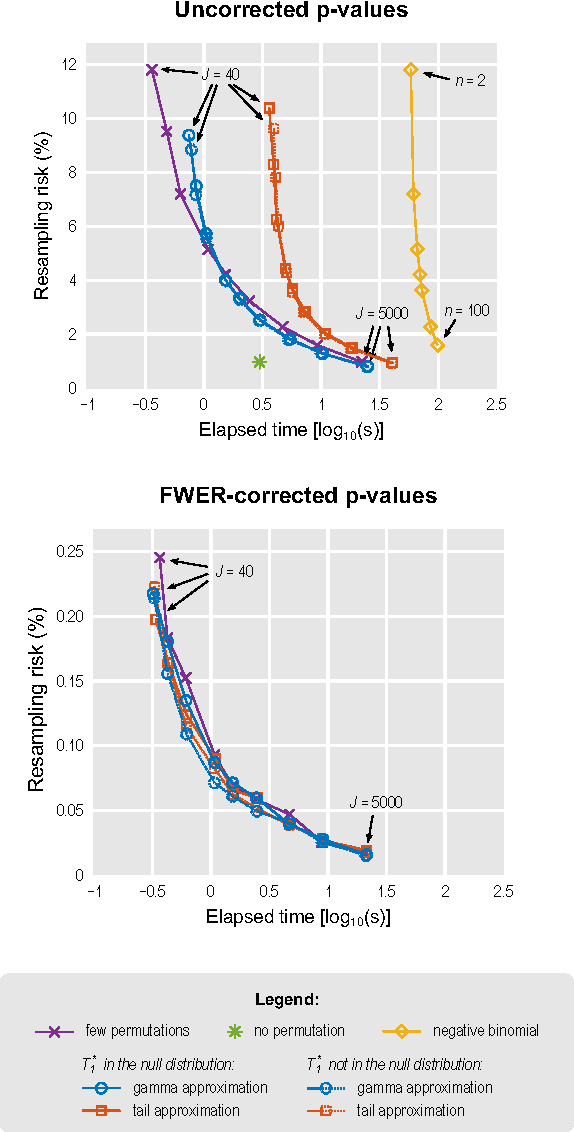
\includegraphics{figures/risk+timing_vert.pdf}
\end{center}
\label{fig:risk+timing_noref}
\end{figure}

\paragraph{Speed} For comparable resampling risks, the method in which no permutations are performed was the absolute fastest. Few permutations, gamma and tail approximations were generally quick, with tail being slower than gamma for the same number of permutations, and gamma slightly slower than few permutations. This considers a voxelwise fit, for uncorrected p-values; if only corrected p-values are needed, the time needed for the single fit of the \textsc{gpd} or gamma for the distribution of extremum statistic is negligible. The negative binomial and, specially, low rank matrix completion were the slowest. Low rank, however, is expected to perform better in settings where there are more tests to be performed (more voxels) than those used in the simulations and real data, and with a relatively smaller sample size (Table~\ref{tab:complexity}).

\paragraph{Noise distribution and shuffling strategy} The performance of the various methods was similar in terms of error rates, power, resampling risk, and speed, regardless of the errors being Gaussian or Weibull (skewed). However, as expected given its assumptions, the method in which no permutations are used did not produce correct results that could be compared with the reference set if the reference set used sign-flippings (for either error distribution), or if the errors were skewed (regardless of the shuffling strategy, i.e., permutations, sign-flippings, or permutations with sign-flippings).

\paragraph{Spatial statistics} The behaviour for spatial statistics followed the same trends as for the voxelwise, non-spatial statistics, in terms of error rates, power, agreement with the reference set, and resampling risk.

\paragraph{Multivariate statistics and non-parametric combination} Likewise, the results for \textsc{cmv} and for \textsc{npc} followed similar trends as above, with error rates controlled exactly, and yielding similar power as the reference set, as evidenced by the results of Phase \textsc{i} shown in the Supplementary Material.

\paragraph{Real data} All methods yielded visually similar maps for the real data, with smaller p-values observable with more permutations for the methods that use permutations, or more exceedances for the negative binomial. In the \textsc{tfce}, \textsc{fwer}-corrected maps, stronger effects of interest could be revealed by tail and gamma methods for equivalent $J$ of few permutations. These results are remarkably similar to the results seen in the reference set, even using about a hundred times fewer permutations, with proportional increases in speed, as summarised in Figures~\ref{fig:vbm-vox-uncp} and~\ref{fig:vbm-tfce-fwep}, and shown in greater detail in the Supplementary Material. The timings refer to the implementation available in \textsc{palm}, as described in Chapter~\ref{sec:conclusion}. The acceleration methods worked similarly, and yielded similar increases in speed, for the two levels of smoothing considered.

\begin{figure}[!b]
\centering
\caption[Uncorrected \textsc{vbm} results, showing the overall amount of time taken by each method.]{\emph{(page \pageref{fig:vbm-vox-uncp_noref})} \textsc{vbm} results, showing \textbf{uncorrected} p-value maps (axial slices $z=10$ and $z=48$~mm, \textsc{mni} space), and the overall amount of time taken by each method. The tail and gamma methods generally have higher power compared to few permutations with the same $J$, even with these not including the unpermuted statistic in the null distribution; see the Supplementary Material for other maps.}
\label{fig:vbm-vox-uncp}
\end{figure}

\begin{figure}[!b]
\centering
\caption[Corrected \textsc{vbm} results, showing the overall amount of time taken by each method.]{\emph{(page \pageref{fig:vbm-tfce-fwep_noref})} \textsc{vbm} results, showing \textbf{corrected} (\textsc{fwer}) p-value \textsc{tfce} maps (axial slices $z=10$ and $z=48$~mm, \textsc{mni} space), and the overall amount of time taken by each method. As with the uncorrected, the methods generally have higher power compared to few permutations with the same $J$, and approximate better the reference set.}
\label{fig:vbm-tfce-fwep}
\end{figure}

\begin{figure}[!tp]
\centering
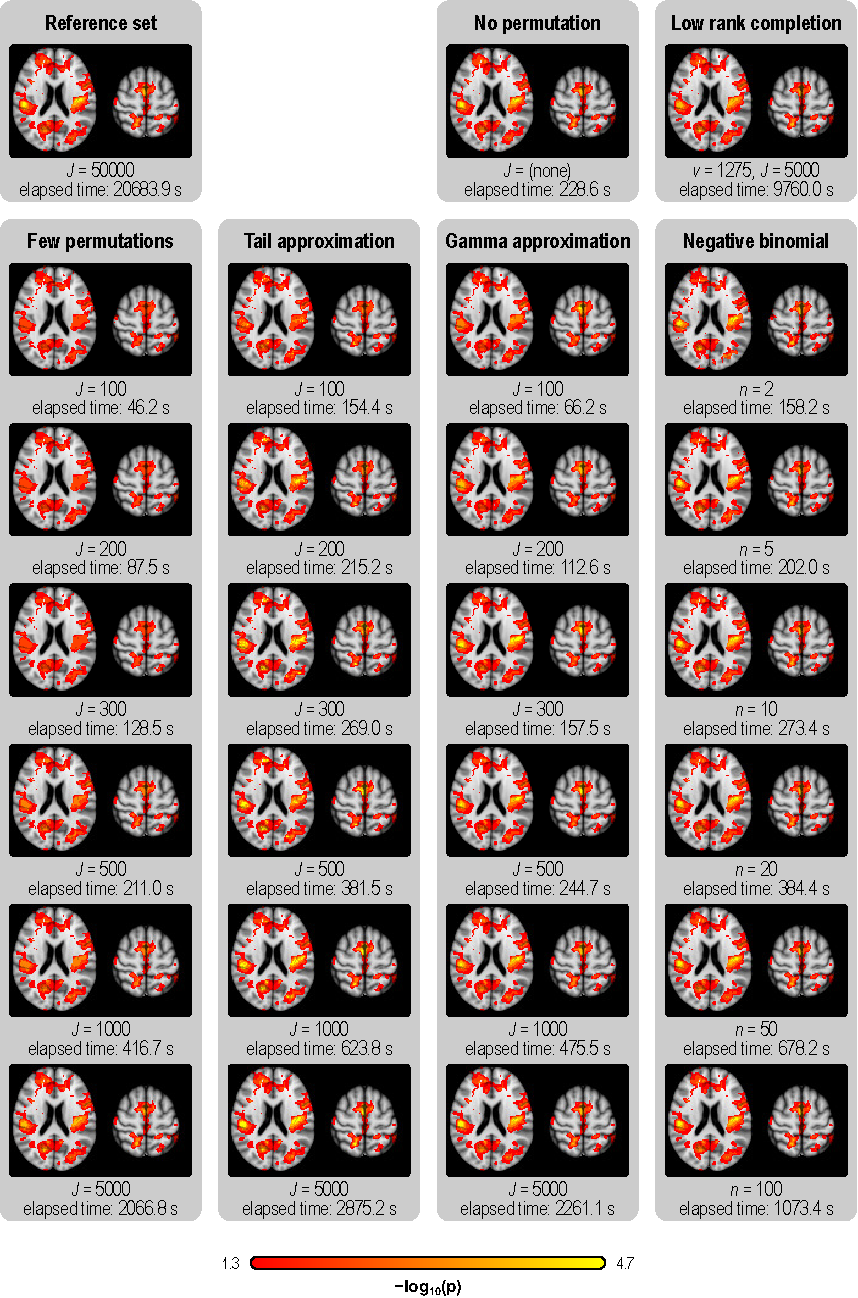
\includegraphics[scale=.9]{figures/vbm-vox-uncp.pdf}
\label{fig:vbm-vox-uncp_noref}
\end{figure}

\begin{figure}[!tp]
\centering
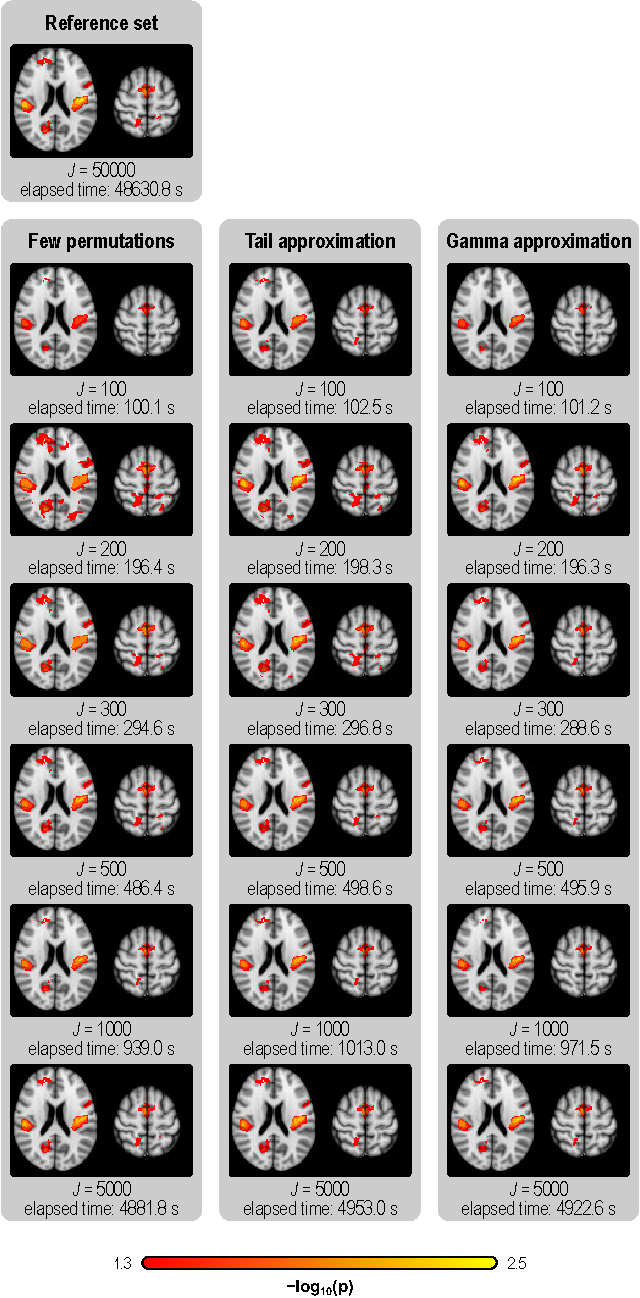
\includegraphics[scale=.9]{figures/vbm-tfce-fwep.pdf}
\label{fig:vbm-tfce-fwep_noref}
\end{figure}

\section{Discussion}

\subsection{Assumptions}

All six methods presented are non-parametric in the sense that they do not depend on the distribution of the test statistic. Some of the methods can still be said to be parametric in that certain parameters need to be estimated, such as for the gamma or for the generalised Pareto distribution, although they remain non-parametric in that the distribution from which these parameters are estimated is based on permutations (or at least conceptually, as in the case of the no permutation method). Some methods nevertheless require certain assumptions: for the gamma approximation, a fit can only be adequate if the distribution of the test statistic is unimodal; for the method in which no permutations are performed, the results are an approximation only to permutations proper, not to sign-flippings, and only if the distribution of the errors is symmetric.

\subsection{Resampling risk and number of permutations}

Although the p-values can vary considerably between the methods, as evidenced by the Bland--Altman plots, at the tails they are remarkably similar, thus allowing similar inferences to be drawn, and presenting an overall low resampling risk for the corrected maps. This means that for most methods, the overall result upon rejection or not of the null hypothesis is expected to remain broadly the same.

The results permit relaxing the usual common sense that more permutations are better. Although more permutations do reduce the resampling risk, the high computational cost may not bring additional information upon acceptance or rejection of the null hypotheses, even considering the large number of tests usually performed in brain imaging. This is particularly the case for \textsc{fwer} corrected results, for which the resampling risk, even for moderate to small number of permutations, was quite small.

It should be noted that, although more permutations do not intrinsically increase power, they allow smaller p-values to be found (Equation~\ref{eqn:pvalue}). Even though p-values much smaller than needed to reach a decision on the null hypotheses may be not needed, such as for \textsc{fwer} correction, methods that use uncorrected p-values as a starting point for further computations, such as for subsequent \textsc{fdr} correction, stand to benefit more from the greater resolution and potentially greater significance of p-values derived with a larger number of permutations. This compounds with more accurate fitting of a distribution, such as the \textsc{gpd} (tail) and gamma, enabled by the larger number of points available in the empirical distribution.

\subsection{Tail, gamma, and no permutation}

For tail and gamma approximations, a small number of permutations is initially performed, from which a low resolution null distribution is built and used for the \textsc{gpd} (tail) or gamma (full distribution) fit. The results show that inclusion or not of the unpermuted test statistic ($T^*_1$) in this null distribution makes a substantial difference in the uncorrected case if too few permutations are performed, with p-values that, at the tail, are either conservative (if included) or invalid (if not included). Thus, if interest lies solely on uncorrected p-values, such as in the absence of multiple testing, or for subsequent use of \textsc{fdr}, other acceleration methods that do not suffer from either conservativeness or invalidity at the tails are advisable. For \textsc{fwer}-corrected p-values, as the number of tests (voxels) increase, the difference between including or not the unpermuted statistic in the null distribution becomes negligible.

This is not an unexpected finding, particularly for test statistics that happen to be at the tail, such as when there is a true, strong effect of interest: by being at the tail, $T^*_1$ is among the rarest values found with the permutations, hence a single extra observation of the statistic is considerably influential if too few permutations are done; for test statistics lying towards the mode of the distribution, where most of the other values are located, a single extra observation has little noticeable effect.

These two methods allow p-values to extend further into the tail of the null distribution than otherwise is possible when only few permutations are used, and are particularly useful for the \textsc{fwer} case, offering a complement for the no permutation method, that is available to produce uncorrected p-values. The latter, however, requires both symmetric error terms and that the intercept is entirely contained in $\mathbf{Z}$. Tail and gamma approximation can also be used even if the number of permutations is reasonably large (such as 5000), yielding corrected results that are remarkably similar to what would be obtained with far more shufflings.

\subsection{Low rank matrix completion}

Various methods can be considered that could make use of low rank matrix completion. The method proposed here performs completion of two matrices, using the data from potentially far fewer tests (voxels) than those present in an image. While completing two matrices, instead of only one, may seem an undesirable computational cost, by restricting the completion to only matrices that can be constructed through linear operations on the data and model, exact recovery is possible. Therefore, problems with unrecoverable residuals due to imperfect reconstruction of the matrix that stores the statistic itself are eschewed, and no assumptions need to be introduced, such as for \emph{ad hoc} attempts for the recovery of the residuals themselves, or for the characterisation of its parameters. The conditions for completion are easily attainable in brain imaging, and the method produces identical results to those obtained with the conventional permutation test.

The method is expected to perform faster with large images and with small samples, although performance gains also need a fast implementation. The simulations were too expensive to use a sufficiently large image, hence potential advantages of low rank completion could not be illustrated. Yet, the method remains an option as  a potential replacement for simple permutations, and as the initial step for tail and gamma approximations. It has also the benefit that, from the recovered statistics, spatial statistics can further be calculated, although direct recovery of such spatial statistics, that are not linear functions of the data, would require approximated results.

\subsection{Applicability}

Most of the assessed methods are generic and can accommodate many cases of potential interest. In particular, the tail and gamma approximations, as well as few permutations, can be applied in a variety of situations that include univariate and multivariate tests (both \textsc{cmv} and \textsc{npc}), spatial statistics, and for the correction using the distribution of the extremum statistic (minimum or maximum). The low rank matrix completion, by producing identical result to few permutations, can likewise be considered a generic solution, although its computational benefits only arise for large images and with relatively smaller sample sizes, and even so, only for univariate statistics.

Except for the method in which no permutations are performed, all others can be considered for experiments that use non-independent data, as long as dependencies between observations have been taken into account by means of exchangeability blocks, including multiple levels of exchangeability \citep{Winkler2015}, with the consequence that these acceleration methods can be used for experiments that used repeated measurements, heterogeneous variances, or other types of structured dependencies.

\subsection{Real data}

Using a \textsc{vbm} dataset was especially useful as this imaging method is known to suffer from non-normality, particularly skewness, and spatial non-stationarity, which could pose difficulties. Yet, the acceleration methods performed generally well, and the results of the reanalysis are in line with those of the original study \citep{Douaud2007}. Of note, at $J=500$, the tail approximation seemed to produce spatial results closer to the reference set than the gamma approximation, with fewer false positives and importantly fewer false negatives in relation to that set, especially in the left Broca's area and the inferior temporal gyri. Using of any of the acceleration methods that can produce \textsc{fwer}-corrected p-values resulted in the same conclusions about rejection of the null, only with considerable increases in speed. Even though the method in which no permutations are done worked reasonably well with the real and presumably skewed \textsc{vbm} data, it should be noted that assumptions were violated, and this method should not in general be recommended in the presence of skewness.

\subsection{Recommendations}

As a general rule, given its generalisability, its lack of dependence on symmetry or on unimodality of the permutation distribution, the need to consider the multiplicity of tests in brain imaging, its availability not only for univariate tests, but also \textsc{cmv} and \textsc{cmv}, as well as spatial statistics, and in the absence of any reasonable information about the data, the tail approximation can be in general recommended. The gamma approximation can be recommended for the same circumstances, and it tends to be slightly faster than the tail approximation, although it requires that the whole permutation distribution is well behaved, and the assumption that its entirety can be approximated by a gamma distribution.

For uncorrected p-values, and without spatial statistics, if symmetry of the error terms can be assumed, the method in which no permutations are performed can be recommended, given its speed. If symmetry cannot be assumed, negative binomial distribution and tail approximation can be used; for the latter, the unpermuted statistic may be excluded from the null distribution if the number of permutations is large given the significance level (such as about a thousand for an $\alpha=0.05$, as considered in the \href{sec:accel:evaluation}{Evaluation}), or if the approximation is used for \textsc{fwer} corrected p-values. The low rank matrix completion can be considered when the number of tests (voxels) is much larger than the number of subjects, as a replacement to the few permutations or to build the initial null distribution before tail or gamma approximations.

As for the number of shufflings to be used, the choice depends on how small the p-value needs to be for a given significance level while maintaining a reasonably small resampling risk. The results seem to indicate that, even without tail or gamma approximations, using about 500 permutations can give stable results for \textsc{fwer} corrected inference, although whenever computational resources are available, more should be considered. The fitting of a \textsc{gpd} or gamma distributions can help with the discreteness that can render \textsc{fdr} conservative. A flow chart summarising these recommendations is shown in Figure~\ref{fig:recomm}.

\begin{figure}[!tp]
\begin{center}
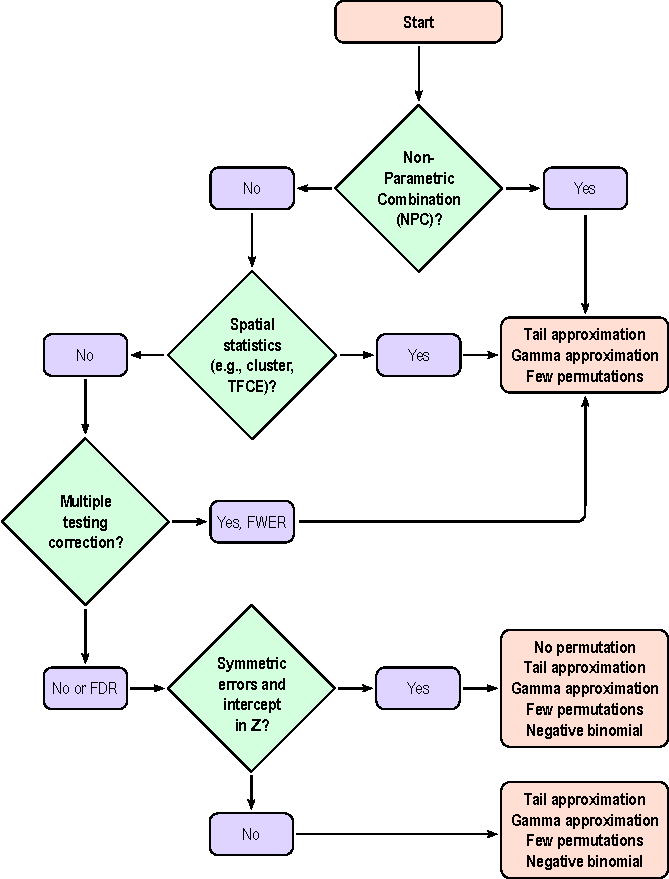
\includegraphics{figures/recomm.pdf}
\end{center}
\caption[Decision tree regarding the various acceleration methods.]{Decision tree regarding the various acceleration methods. Each of the terminal boxes show, in order, the preferred methods. For \textsc{npc}, spatial statistics, or for \textsc{fwer}-corrected p-values, tail and gamma approximations, and few permutations are in general recommendead; gamma is faster than tail fitting, but the latter is more generic. For uncorrected p-values, without spatial statistics, and if the errors can be assumed symmetric, the no permutation method is preferred; if symmetry cannot be assumed, the negative binomial is favoured. The low rank matrix completion (not shown) can be used if $N \ll V$, as a replacement to the few permutations or to build the initial null distribution before tail or gamma approximations.}
\label{fig:recomm}
\end{figure}

\cleardoublepage \chapter{Permutation tests for cortical morphometry}
\label{sec:cortex}
\setstretch{\lspac}

\section{Introduction}
\label{sec:cortex:intro}
\setstretch{\lspac}

It has been suggested that biological processes that drive horizontal (tangential) and vertical (radial) development of the cerebral cortex are separate from each other \citep{Rakic1988,Geschwind2013}, influencing cortical area and thickness independently. These two indices of cerebral morphology are uncorrelated genetically \citep{Panizzon2009, Winkler2010}, are each influenced by regionally distinct genetic factors \citep{Schmitt2008, Rimol2010_bp, Chen2012, Chen2015}, follow different trajectories over the lifespan \citep{OLeary2007, Hogstrom2013, Fjell2015}, and are differentially associated with cognitive abilities and disorders \citep{Schnack2015, Noble2015, Lee2016, Vuoksimaa2016}. Moreover, it is cortical area, not thickness, that differs substantially across species \citep{Rakic1995}. These findings give prominence to the use of surface area alongside thickness in studies of cortical morphology and its relationship to function. The literature contains a variety of approaches and terminologies for its assessment and cortical volume, which commingles thickness and area, continues to be a popular metric, thanks largely to the wide availability of voxel-based morphometry (\textsc{vbm}) \citep{Ashburner2000, Good2001, Douaud2007}. While analysing cortical thickness and cortical area separately improves specificity \citep{Rimol2012}, it may still be of interest to combine these two measurements so as to increase power to investigate non-specific challenges that could affect thickness and area simultaneously, such as auto-immune \citep{Ceccarelli2008, Zhang2016} and infectious neurological disorders \citep{Gitelman2001, Kuper2011}, or in relation to inflammatory markers \citep{Marsland2008, Zhang2015}. The contributions of this chapter are threefold: we (\textsc{i}) expose certain aspects of the various methods for cortical area analysis, in particular the interpolation between surfaces at different resolutions; (\textsc{ii}) propose an improved, analytic measurement of volume; (\textsc{iii}) show that a joint analysis using the non-parametric combination \textsc{npc} \citep{Pesarin2010, Winkler2016_npc} of thickness and area provides a sensible solution to the investigation of factors that may affect cortical morphology, which can replace the analysis of cortical volume altogether.
 
\subsection{Cortical surface area}

Using continuous cortical maps to compare surface area across subjects offers advantages over a region-of-interest (\textsc{roi}) approach, since it does not require that the effects map onto a previously defined \textsc{roi} scheme. For instance, a group difference present in a subregion of a given \textsc{roi} may be cancelled out by the absence of a difference in the rest of the \textsc{roi} and thus remain undetected. Nevertheless, surface area analyses still depend on registration of the cortical surface and interpolation to a common resolution. Such resampling must preserve the amount of area at local, regional and global scales, i.e., it must be mass-conservative. A well known interpolation method is the \emph{nearest-neighbour}, which can be enhanced by correction for stretches and shrinkages of the surface during the registration, as available in the function \texttt{mris\_preproc}, part of the FreeSurfer (\textsc{fs}) software package.\footnote{Available at \href{http://freesurfer.net}{freesurfer.net}} Another approach is the \emph{retessellation} of the mesh of each subject to the geometry of a common grid, as proposed by \cite{Saad2004} as a way to produce meshes with similar geometry across subjects, and as available in the package \textsc{afni/suma}. \footnote{Available at \href{https://afni.nimh.nih.gov}{afni.nimh.nih.gov}} Even though the method has been mostly used to compute areal expansion, it can be used for surface area itself, as well as for other areal quantities. A third approach is the use of the barycentric coordinates of each vertex with reference to the vertices of the common grid to \emph{redistribute} the areal quantities, in an approximately mass preserving process. Lastly, a strategy for analysis of areal quantities was presented in \cite{Winkler2012} using a \emph{pycnophylactic} (mass-preserving) interpolation method (Table~\ref{tab:overview}).

\begin{table}[!tp]
\caption[Overview of the four different methods to interpolate surface area and areal quantities.]{Overview of the four different methods to interpolate surface area and areal quantities. A detailed description is in Section~\ref{sec:cortex:methods}.}
\begin{center}
\begin{small}
\begin{tabular}{@{}m{28mm}<{\raggedright}m{96mm}<{\raggedright}@{}}
\toprule
\textbf{Method} & \textbf{Description} \\ 
\midrule
Nearest-neighbour & Nearest-neighbour interpolation of areal quantities on the sphere, followed by Jacobian correction.\\
\midrule
Retessellation & Barycentric interpolation on the sphere of the native vertex coordinates.\\
\midrule
Redistributive & Vertexwise redistribution of areal quantities based on bary\-centric coordinates of the source in relation to the target.\\
\midrule
Pycnophylactic & Mass-conservative facewise interpolation method that uses the overlapping areas between faces of source and target.\\
\bottomrule
\end{tabular}
\end{small}
\end{center}
\label{tab:overview}
\end{table}

\subsection{Measuring volume and other areal quantities}

The volume of cortical grey matter is also an areal quantity, which therefore requires mass-conservative interpolation methods. Volume can be estimated through the use of voxelwise partial volume effects using volume-based representations of the brain, such as in \textsc{vbm}, or from a surface representation, in which it can be measured as the amount of tissue present between the surface placed at the site of the pia-mater, and the surface at the interface between gray and white matter. If the area of either of these surfaces is known, or if the area of a mid-surface, i.e., the surface running half-distance between pial and white surfaces \citep{vanEssen2005} is known, an estimate of the volume can be obtained by multiplying, at each vertex, area by thickness. This procedure, while providing a reasonable approximation that improves over voxel-based measurements, since it is less susceptible to various artefacts \cite[for a discussion of artefacts in \textsc{vbm}, see][]{Ashburner2009}, is still problematic as it underestimates the volume of tissue that is external to the convexity of the surface, and overestimates volume that is internal to it; both cases are undesirable, and cannot be solved by merely resorting to using an intermediate surface as the mid-surface (Figure~\ref{fig:mantle}a). Here a different approach is proposed: each face of the white surface and its matching face in the pial surface are used to define an oblique truncated pyramid, the volume of which is computed analytically, without introducing additional error other than what is intrinsic to the placement of these surfaces (Figure~\ref{fig:mantle}b for a 2-\textsc{d} schema and Figure~\ref{fig:pyramid} for 3-\textsc{d}).

\begin{figure}[!tp]
\begin{center}
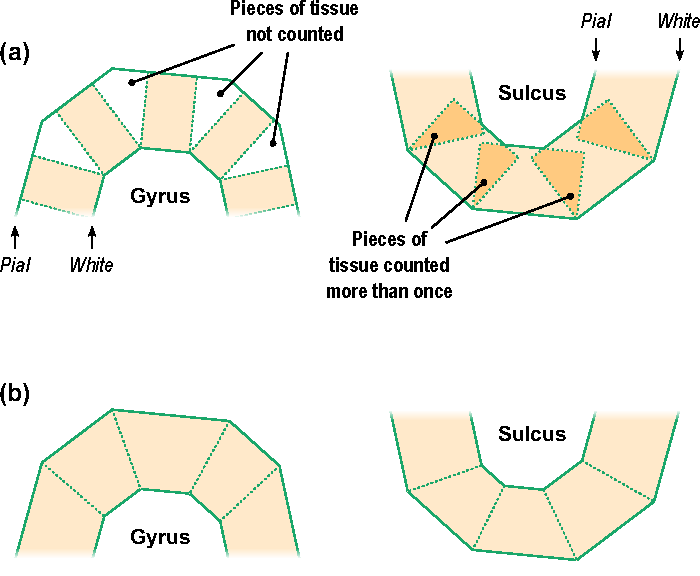
\includegraphics[scale=.9]{figures/mantle.pdf}
\caption[A \textsc{2-d} diagram of the problem of measuring the cortical volume.]{A diagram in two dimensions of the problem of measuring the cortical volume. (\emph{a}) If volume is computed using multiplication of thickness by area, considerable amount of tissue is left unmeasured in the gyri, or measured repeatedly in sulci. The problem is minimised, but not solved, with the use of the mid-surface. (\emph{b}) Instead, vertex coordinates can be used to compute analytically the volume of tissue between matching faces of white and pial surfaces, leaving no tissue under- or over-represented.}
\label{fig:mantle} 
\end{center}
\end{figure}

\begin{figure}[!tp]
\begin{center}
\includegraphics[width=\textwidth]{figures/pyramid.pdf}
\caption[A \textsc{3-d} diagram with the proposed solution to measure the cortical volume.]{(\emph{a}) In the surface representation, the cortex is limited internally by the white and externally by the pial surface. (\emph{b}) and (\emph{c}) These two surfaces have matching vertices that can be used to delineate an oblique truncated triangular pyramid. (\emph{d}) The six vertices of this pyramid can be used to define three tetrahedra, the volumes of which are computed analytically.}
\label{fig:pyramid}
\end{center}
\end{figure}

Quantitative measurements, such as from positron emission tomography (\textsc{pet}), cerebral blood flow, cerebral blood volume, the mass, or number of molecules of a given compound \citep{Leahy2000, VandenHoff2005}, are all areal quantities whenever these are expressed in absolute quantities. Likewise, cerebral blood flow and volume obtained using methods based on magnetic resonance imaging (\textsc{mri}), such as arterial spin labelling (\textsc{asl}), as well as other forms of quantitative \textsc{mri}, as those involving contrast enhancement \citep{Parker2003}, quantitative magnetisation transfer \citep{Levesque2010, Harrison2015}, or quantitative assessment of myelination, are also areal quantities that require mass conservation when measured in absolute terms. The methods used for statistical analysis surface area can be applied for these areal quantities as well.

\subsection{Non-parametric combination (\textsc{npc})}

Instead of volume, we suggest that a joint approach can be used for the analysis of thickness and area. Classical multivariate tests such as \textsc{mancova}, however, are not informative about the direction of any observed effects, and are based on assumptions that are known not to hold for surface area, such as normality. Rather, the permutation-based non-parametric combination (\textsc{npc}) \citep{Pesarin2010, Winkler2016_npc} provides a test for directional as well as two-tailed hypotheses, and is based on minimal assumptions, mainly that of exchangeability, that is, swapping one datum for another keeps the data just as likely. The \textsc{npc} consists of, in a first phase, testing separately hypotheses on each available metric using permutations that are performed in synchrony; these tests are termed \emph{partial tests}. The resulting statistics for each and every permutation are recorded, allowing an estimate of the complete empirical cumulative distribution function (cdf) to be constructed for each one. In a second phase, the empirical p-values for each test are combined, for each permutation, into a \emph{joint statistic}. As the joint statistic is produced from the previous permutations, an estimate of its empirical cdf function is immediately known, and so is its corresponding p-value \citep{Pesarin2010}.

As originally proposed, and as described above, \textsc{npc} is not practicable in brain imaging: as the statistics for all partial tests for all permutations need to be recorded, an enormous amount of space for data storage is necessary. However, even if storage space were not a problem, the discreteness of the p-values for the partial tests is problematic when correcting for multiple testing, because with thousands of vertices in a surface, ties occur frequently, further causing ties among the combined statistics. If too many tests across an image share the same most extreme statistic, correction for the multiplicity, while still valid, is less powerful \citep{Westfall1993, Pantazis2005}. The most obvious workaround --- run an ever larger number of permutations to break the ties --- may not be possible for small sample sizes, or when possible, requires correspondingly larger data storage. The solution to this problem is loosely based on the direct combination of the test statistics, by converting the statistics of the partial tests to values that behave as p-values using the asymptotic distribution of the statistics, and using these for the combination \citep{Winkler2016_npc}.

\paragraph{Combining functions}

The null hypothesis of the \textsc{npc} is that the null hypotheses for all partial tests are true, and the alternative is that any test is false, which is the same that a union-intersection test (\textsc{uit}) \citep{Roy1953}. The rejection region depends on how the combined statistic is produced. Various combining functions can be considered, particularly those used in meta-analyses, such as Fisher's combination of p-values, i.e., $T=-2\sum_k\ln(p_k)$ \citep{Fisher1932} and Stouffer's combination of $z$-statistics, i.e., $T = \sum_k \Phi^{-1}(1-p_k)/\sqrt{K}$ \citep{Stouffer1949}, where $T$ is the test statistic for the joint test, $p_k$ is the p-value of the $k$-th out of $K$ partial tests, and $\Phi^{-1}$ is the probit function. These and most other combining functions, related statistics and their distributions were originally derived under the assumption of independence among the partial tests, which is not always valid, particularly under the tenable hypothesis of shared environmental effects affecting both area and thickness. Such lack of independence is not a problem for \textsc{npc}: the synchronised permutations implicitly capture the dependencies among the tests that would cause a parametric combination to be invalid, even if using the same combining functions.

\section{Methods}
\label{sec:cortex:methods}

The general workflow for surface-based morphometry consists of the generation of a surface-representation of the cortex and its subsequent homeomorphic transformation into a sphere. Vertices of this sphere are shifted tangentially along its surface to allow alignment matching a particular feature of interest of a reference brain (i.e., an atlas), such as sulcal depth, myelin content, or functional markers. Once registration has been done, interpolation to a common grid is performed; it is at the resolution of this grid that analyses across subjects are performed. While the order of these processing stages remains generally fixed, the stage in which areal quantities are calculated or obtained varies according to the method: for the nearest neighbour, redistributive, and pycnophylactic methods, these are computed in the native space, using native geometry. With the retessellation method, area is computed in native space, with a new geometry produced after interpolation of the surface coordinates to the common grid. An overview of the whole process is in Figure~\ref{fig:flowchart}.

\begin{figure}[!p]
\begin{center}
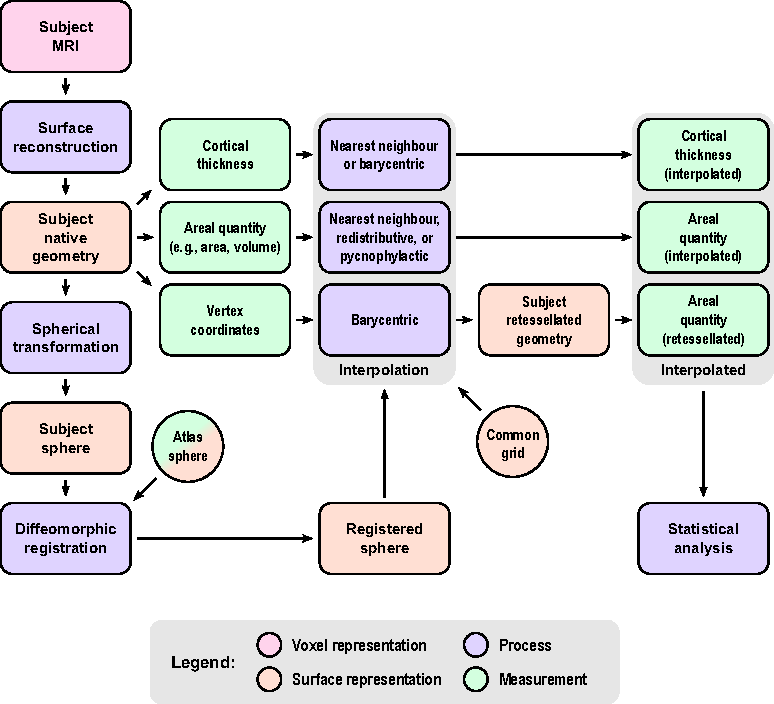
\includegraphics[width=\textwidth]{figures/flowchart.pdf}
\caption[Overview of the steps for the analysis of surface area and thickness using different resampling methods.]{An overview of the steps for the analysis of surface area and thickness using different resampling methods. The subject magnetic resonance images are used to reconstruct a pair of surfaces (pial and white) representing the cortex, which initially are in the subject space and individual geometry. From this pair of surfaces, cortical thickness can be measured. From the same surfaces, area and volume can be measured. Finally, the coordinates of the vertices can be stored for subsequent use. The subject native surfaces are homeomorphically transformed to a sphere, registered to a spherical atlas, and used for the interpolation, which for thickness can be either nearest neighbour or barycentric, for area can be nearest neighbour, redistributive or pycnophylactic, and for the vertex coordinates can be barycentric. In the latter, the interpolation of coordinates allows the construction of a new retessellated surface in subject space, from which area can alternatively be measured. The interpolated quantities are then ready to undergo statistical analyses. See references in the main text.}
\label{fig:flowchart}
\end{center}
\end{figure}

We evaluate (\textsc{i}) if and where the four different interpolation methods (nearest neighbour, retessellation, redistributive and pycnophylactic) differ; (\textsc{ii}) if and where these methods vary according to the resolution of the common grid used as target; (\textsc{iii}) if and where the two ways of measuring volumes (the product method and the analytic method) differ from each other; (\textsc{iv}) how the \textsc{npc} results would relate to the separate analyses of thickness, area and volume.

\subsection{Subjects}

In the period 1986--88, 121 preterm newborns with very low birth weight (\textsc{vlbw}; $\leqslant$~1500g) were admitted to the Neonatal Intensive Care Unit at the St.\ Olav University Hospital in Trondheim, Norway. At age 20, a total of 41 \textsc{vlbw} subjects consented to participate and had usable \textsc{mri} data. The term-born controls were born at the same hospital in the same period. A random sample of women with parities 1 or 2 was selected for follow-up during pregnancy. At birth, 122 children with birth weight above the tenth percentile for gestational age from this sample were included as controls. At age 20, a total of 59 control subjects consented to participate and had usable \textsc{mri} data. Further details can be found in \citet{Martinussen2005, Skranes2007}.

\subsection{Data acquisition}

\textsc{mri} scanning was performed on a 1.5~T Siemens \textsc{magnetom} Symphony scanner equipped with a quadrature head coil. In each scanning session, two sagittal $T_1$-weighted magnetization prepared rapid gradient echo (\textsc{mprage}) scans/sequences were acquired (echo time = 3.45~ms, repetition time = 2730~ms, inversion time = 1000~ms, flip angle = 7\degree; field of view = 256~mm, voxel size = 1 $\times$ 1 $\times$ 1.33~mm, acquisition matrix 256 $\times$ 192 $\times$ 128).  

\subsection{Reconstruction of the cortical surface}

We used the method implemented in the FreeSurfer software package \cite[version 5.3.0;][]{Dale1999,Fischl1999_cortical}: $T_1$-weighted images are first corrected for magnetic field inhomogeneities and then skull-stripped \citep{Segonne2004}. Voxels belonging to the white matter (\textsc{wm}) are identified based on their locations, on their intensities, and on the intensities of the neighbouring voxels. A mass of connected \textsc{wm} voxels is produced for each hemisphere, using a six-neighbours connectivity scheme, and a mesh of triangular faces is tightly built around this mass, using two triangles for each externally facing voxel side. The mesh is smoothed taking into account the local intensity in the original images \citep{Dale1993}, at a subvoxel resolution. Defects are corrected \citep{Fischl2001,Segonne2007} to ensure that the surface has the same topological properties of a sphere. A second iteration of smoothing is applied, resulting in a realistic representation of the interface between gray and white matter (the \emph{white surface}). The external cortical surface (the \emph{pial surface}), which corresponds to the pia mater, is produced by nudging outwards the white surface towards a point where the tissue contrast is maximal, between gray matter and \textsc{csf}, maintaining constraints on its smoothness while preventing self-intersection. Cortical thickness is measured as the distance between the matching vertices of these two surfaces \citep{Fischl2000}.

\subsection{Measurement of areal quantities}

Areal quantities are measured in native space, i.e., before spherical transformation and registration. For the retessellation method, the measurement is made in native space after the surface has been reconstructed to a particular resolution; for nearest neighbour, redistributive, and pycnophylactic, measurement uses native space, with the original, subject-specific mesh geometry. 

\paragraph{Cortical area}

For a triangular face $ABC$ of the surface representation, with vertex coordinates $\mathbf{a}=[x_A \; y_A \; z_A]'$, $\mathbf{b}=[x_B \; y_B \; z_B]'$, and $\mathbf{c}=[x_C \; y_C \; z_C]'$, the area is $|\mathbf{u} \times \mathbf{v}|/2$, where $\mathbf{u} = \mathbf{a}-\mathbf{c}$, $\mathbf{v} = \mathbf{b}-\mathbf{c}$, $\times$ represents the cross product, and the bars $|\;|$ represent the vector norm. Although the area per face (i.e., the \emph{facewise} area) can be used in subsequent steps, it remains the case that most software packages can only deal with values assigned to each vertex of the mesh (i.e., \emph{vertexwise}). Conversion from facewise to vertexwise is achieved by assigning to each vertex one-third of the sum of the areas of all faces that have that vertex in common \citep{Winkler2012}.

\paragraph{Cortical volume}

The conventional method for computing surface-based volume consists of computing the area at each vertex as above, then multiplying this value by the thickness at that vertex, in a procedure that leaves tissue under- or over-represented in gyri and sulci (Figure~\ref{fig:mantle}). Instead, volumes can be computed using the three vertices that define a face in the white surface and the three matching vertices in the pial surface, defining an \emph{oblique truncated triangular pyramid}, which in turn is perfectly subdivided into three tetrahedra. The volumes of these are computed analytically, summed, and assigned to each face of the surface representation, viz.:

\begin{itemize}[leftmargin=*]
\item[1.] For a given face $A_w B_w C_w$ in the white surface, and its corresponding face $A_p B_p C_p$ in the pial surface, define an oblique truncated triangular pyramid.
\item[2.] Split this truncated pyramid into three tetrahedra, defined as:
$$
\begin{array}{lcllllll}
T_1 &=& (&A_w,&B_w,&C_w,&A_p&)\\
T_2 &=& (&A_p,&B_p,&C_p,&B_w&)\\
T_3 &=& (&A_p,&C_p,&C_w,&B_w&)
\end{array}$$
This division leaves no volume under- or over-represented.
\item[3.] For each such tetrahedra, let $\mathbf{a}$, $\mathbf{b}$, $\mathbf{c}$ and $\mathbf{d}$ represent its four vertices in terms of coordinates $[x\;y\;z]'$. Compute the volume as $|\mathbf{u}\cdot(\mathbf{v} \times \mathbf{w})|/6$, where $\mathbf{u} = \mathbf{a}-\mathbf{d}$, $\mathbf{v} = \mathbf{b}-\mathbf{d}$, $\mathbf{w} = \mathbf{c}-\mathbf{d}$, the symbol $\times$ represents the cross product, $\cdot$ represents the dot product, and the bars $|\;|$ represent the vector norm.
\end{itemize}

\noindent
Computation can be accelerated by setting $\mathbf{d}=A_p$, the common vertex for the three tetrahedra, such that the vector subtractions can happen only once. Conversion from facewise volume to vertexwise is possible, and done in the same manner as for facewise area. The above method will be the default in the next FreeSurfer release.

\subsection{Spherical transformation}

The white surface is homeomorphically transformed to a sphere \citep{Fischl1999_intersubject}, thus keeping a one-to-one mapping between faces and vertices of the native geometry (white and pial) and the sphere. All these surfaces comprise triangular faces exclusively. Measurements of interest obtained from native geometry or in native space, such as area and thickness, are stored separately and are not affected by the transformation, nor by registration (next step; see diagram in Figure~\ref{fig:flowchart}).

\subsection{Registration}

Various strategies are available to place all surfaces in register and allow inter-subject comparisons, including the ones used by FreeSurfer \citep{Fischl1999_intersubject}, Spherical Demons (\textsc{sd}) \citep{Yeo2010}, Multimodal Surface Matching (\textsc{msm}) \citep{Robinson2014}, among others. Methods that are diffeomorphic (i.e., smooth and invertible) should be favoured. Methods that are not diffeomorphic by design but in practice produce invertible and smooth warps can, in principle, be used in registration for areal analyses. In the present analyses, FreeSurfer was used; a side comparison with \textsc{sd} is in Appendix \ref{sec:supplmat}.4.1).

\subsection{Interpolation methods}
\label{sec:cortex:interpolation}

Statistical comparisons require meshes with a common resolution where each point (vertex, face) represents homologous locations across individuals. One type of mesh that can act as a common grid is a geodesic sphere constructed by iterative subdivision of the faces of a regular (Platonic) icosahedron. A geodesic sphere has many advantages as the target for interpolation: ease of computation, edges of roughly similar sizes and, if the resolution is fine enough, edge lengths that are much smaller than the diameter of the sphere \citep{Kenner1976}. We compared four different interpolation methods each at three different mesh resolutions: \textsc{ic}3 (lowest resolution, with 642 vertices and 1280 faces), \textsc{ic}5 (intermediate resolution, with 10242 vertices and 20480 faces),  and \textsc{ic}7 (163842 vertices and 327680 faces).

\paragraph{Nearest neighbour interpolation}

The well known nearest neighbour interpolation does not guarantee preservation of areal quantities, although modifications can be introduced to render it approximately mass conservative: for each vertex in the target, the closest vertex is found in the source sphere, and the area from the source vertex is assigned to the target vertex; if a given source vertex maps to multiple target vertices, its area is divided between them so as to preserve the total area. If there are any source vertices that have not been represented in the target, for each one of these, the closest target vertex is located and the corresponding area from the source surface is incremented to any area already stored on it. This method ensures that total area remains unchanged after mapping onto the group surface.  This process is a surface equivalent of Jacobian correction\footnote{Not to be confused with the computation of the Jacobian itself, that is defined, for the $i$-th vertex, as $J_i = \frac{A^S_i}{A^w_i}\frac{\sum_i A^w_i}{\sum_i A^S_i}$, where $A^S_i$ is the area of the vertex in the source (registered) sphere, $A^w_i$ is the area of the same vertex in the white surface (native space and native geometry), and the sums are over the entire surface, i.e., all vertices.} used in volume-based methods in that it accounts for stretches and shrinkages while preserving the overall amount of areal quantities. Nearest neighbour interpolation is currently the default method in FreeSurfer.

\paragraph{Retessellation of the native geometry}

This method appeared in \citet{Saad2004}. It consists of generating a new mesh by interpolating not the area assigned to vertices but the coordinates of the corresponding vertices in the native geometry. The set of three coordinates is used, together with the connectivity scheme between vertices from the common grid, to construct a new mesh that has similar overall shape as the original brain, but with the geometry of the common grid. The area for each face (or vertex) can be computed from this new mesh and used for statistical comparison across subjects. Equivalently, the coordinates of each vertex can be treated as a single vector and the barycentric interpolation can be performed in a single step, as:

$$
\left[
\begin{array}{c}
x_{P} \\
y_{P} \\
z_{P}
\end{array} \right] = \left[
\begin{array}{ccc}
x_{A} & x_{B} & x_{C} \\
y_{A} & y_{B} & y_{C} \\
z_{A} & z_{B} & z_{C} \\
\end{array}
\right] \left[
\begin{array}{c}
\delta_{A} \\
\delta_{B} \\
\delta_{C}
\end{array} \right]
$$

\noindent
where $x,y,z$ represent the coordinates of the triangular face $ABC$ and of the interpolated point $P$, both in native geometry, and $\delta$ are the barycentric coordinates of $P$ with respect to the same face after the spherical transformation. From the four methods considered in this chapter, this is the only one that does not directly interpolate either area or areal quantities, but the mesh in native space.

\paragraph{Redistribution of areas}

This method works by splitting the areal quantity present at each vertex in the source sphere using the proportion given by the barycentric coordinates of that vertex in relation to the face in the target sphere (common grid) on which it lies, redistributing these quantities to the three vertices that constitute that face in the target. If some quantity was already present in the target vertex (e.g., from other source vertices lying on the same target face), that quantity is incremented. The method is represented by:

$$
Q^T_i = \sum_{f=1}^F\sum_{v=1}^{V_f} Q^S_{vf}\delta_{ivf}
$$

\noindent
where $Q^S_{vf}$ is the areal quantity in the source vertex $v$, $v\in\left\{1, \ldots, V_f \right\}$ lying on the target face $f$, $f\in\{1,\ldots,F\}$, $F$ being the number of faces that meet at the target vertex $i$, and $\delta_{ivf}$ is the barycentric coordinate of $v$, lying on face $f$, and in relation to the target vertex $i$. This method has similarities with the conventional barycentric interpolation (as used for the interpolation of coordinates in the retesselation method). The key difference is that in the barycentric interpolation, it is the barycentric coordinates of the target vertex in relation to their containing source face that are used to weight the quantities, in a process that therefore is not mass conservative. Here it is the barycentric coordinates of the source vertex in relation to their containing target face that are used; the quantities are split proportionately, and redistributed across target vertices.

\paragraph{Pycnophylactic interpolation}

The ideal interpolation method should conserve the areal quantities globally, regionally and locally. In other words, the method has to be \emph{pycnophylactic}. This is accomplished by assigning, to each face in the target sphere, the areal quantity of all overlapping faces from the source sphere, weighted by the fraction of overlap between them \citep{Markoff1973, Winkler2012}. The pycnophylactic method operates on the faces directly, not on vertices and the area (or any other areal quantity) is transferred from source to target surface via weighting by the overlapping area between any pairs of faces. The interpolated areal quantity, $Q^{T}_{i}$, of a face $i$ in the target surface, that overlaps with $F$ faces from the source surface, is given by:

$$
Q^{T}_{i} = \sum_{f=1}^{F} \frac{A^{O}_{f}}{A^{S}_{f}} Q^{S}_{f}
$$

\noindent
where $A^{S}_{f}$ is the area of the $f$-th overlapping face from the source sphere, which contains a quantity $Q^{S}_{f}$ of some areal measurement (such as the surface area measured in the native space), and $A^{O}_{f}$ is the overlapping area with the face $i$.

\paragraph{Correction for unequal face sizes and smoothing}

Regardless of the interpolation method used, larger faces in the common grid inherit larger amounts of areal quantities. If the analysis will compare regions that are topographically distinct, or if the data are to be smoothed, a correction for different face sizes is needed \citep{Winkler2012}. For facewise data, such a correction consists of weighting the the areal quantity at each face or vertex, after interpolation, by a constant that depends on the respective area in the common grid. Smoothing was considered at two levels for the comparison of areal interpolation and volume methods: no smoothing, and smoothing with a Gaussian kernel with full width at half maximum (\textsc{fwhm}) of 10~mm, small so as to preserve the effect of different resolutions being investigated. For the comparison between \textsc{vlbw} and controls, 30~mm, as in \citet{Skranes2013}.

\subsection{Statistical analysis}

The statistical analysis was performed using the tool Permutation Analysis of Linear Models \citep[\textsc{palm}; ][see also Section~\ref{sec:conclusion:palm}]{Winkler2014, Winkler2016_npc}. The number of permutations was set to 1000, followed by approximation of the tail of the distribution by a generalised Pareto distribution \citep[\textsc{gpd}; ][see also Chapter \ref{sec:accel}]{Winkler2016_fast}, and familywise error rate correction (\textsc{fwer}) was applied considering both hemispheres and both test directions for the null hypothesis of no difference between the two groups. Analyses were performed separately for cortical thickness, area, and volume (both methods), and also using \textsc{npc} for the joint analysis of thickness and area; see diagram in Figure \ref{fig:flowstats}	.

\begin{figure}[!tp]
\begin{center}
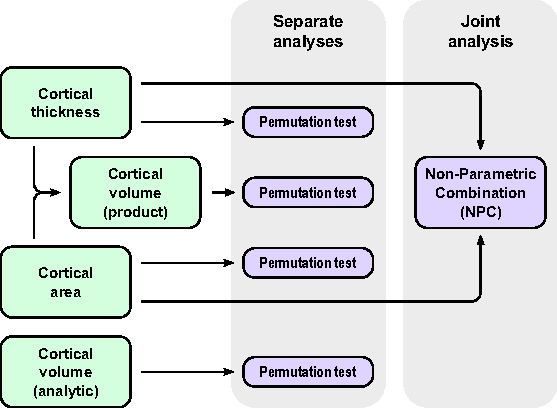
\includegraphics{figures/flowstats.pdf}
\caption[Overview of the separate and joint analyses of thickness, area and volume.]{Overview of the separate and joint analyses of thickness, area and volume.}
\label{fig:flowstats}
\end{center}
\end{figure}

\subsection{Presentation of results}

The large number of scenarios evaluated, that involved two different registration and four different interpolation methods, three grid resolutions, two different smoothing levels, four different indices of cortical morphology, plus \textsc{npc}, resulted in more than 16 thousand maps and Bland-Altman plots \citep{Bland1986}. These have been organised in a set of browsable pages accessible online; see details in Appendix \ref{sec:supplmat}.

\section{Results}
\label{sec:cortex:results}

\subsection{Preservation of areal quantities}

All methods preserve generally well the global amount of surface area, and therefore, of other areal quantities, at the highest resolution of the common grid (\textsc{ic}7). At lower resolutions, massive amounts of area are lost with the retessellation method: about 40\% on average for \textsc{ic}3 (lowest resolution, with 642 vertices and 1280 faces) and 9\% for \textsc{ic}5 (intermediate resolution, with 10242 vertices and 20480 faces), although only 1\% for \textsc{ic}7 (163842 vertices and 327680 faces). Areal losses, when existing, tend to be uniformly distributed across the cortex (Figure~\ref{fig:diff+corr}, upper panels), with no trends affecting particular regions and, except for retessellation, can be substantially alleviated by smoothing (Appendix \ref{sec:supplmat}.4.1). % thus suggesting that quantitatively, pycno is better.

\begin{figure}[!p]
\begin{adjustbox}{addcode={\begin{minipage}{\width}}{
\caption[Pairwise average differences and correlations between the four resampling methods.]{Pairwise average differences (in mm$^2$) and correlations between the four resampling methods, using the \textsc{ic}7 as target, with or without smoothing with a Gaussian kernel of \textsc{fwhm} = 10~mm, projected to the average white surface. Although the four methods differ, with some leading to substantial, undesirable losses and gains in surface area, and the introduction of noise manifested by lower correlations, the average variation was zero for nearest neighbour, redistributive and pycnophylactic. The retessellation method led to substantial losses of area that could not be recovered or compensated by blurring. Although this method showed excellent correlation with pycnophylactic, quantitative results after interpolation are biased downwards. For the medial views, for the right hemisphere, for \textsc{ic}3 and \textsc{ic5}, and for projections to the pial and inflated surfaces, consult Appendix \ref{sec:supplmat}.4.}
\label{fig:diff+corr}
\end{minipage}},rotate=90,center}
\includegraphics[scale=1.1]{figures/diff+corr.pdf}
\end{adjustbox}
\end{figure}

\subsection{Differences between interpolation methods}

While there are no spatial trends in terms of areal gains or losses, the inexactness of the non-pycnophylactic interpolation methods introduces noise that substantially reduces their correlation when assessed between subjects (Figure~\ref{fig:diff+corr}, lower panels). The only exception is between the retessellation and the pycnophylactic methods, which have near perfect correlation even without any smoothing. Smoothing increases the correlation between all methods to near unity throughout the cortex (Appendix \ref{sec:supplmat}.4.1\emph{a}). At the subject level, the spatial correlation between the nearest neighbour and the pycnophylactic methods is only about 0.60, although approaching unity when the subjects are averaged (Appendix \ref{sec:supplmat}.4.1\emph{b}). Smoothing leads to a dramatic improvement on agreement, causing nearest neighbour to be nearly indistinguishable from the pycnophylactic method. The redistributive method performed in a similar manner, although with a higher correlation without smoothing, i.e., about 0.75 (Appendix \ref{sec:supplmat}.4.1\emph{b}).

\subsection{Cortical volume measurements}

At the local scale, differences between the product and the analytic methods of volume estimation are as high as 20\% in some regions (Appendix \ref{sec:supplmat}.4.2), an amount that could not be alleviated by smoothing or by changes in resolution. As predicted by Figure~\ref{fig:mantle}, differences were larger in the crowns of gyri and depths of sulci, in either case with the reverse polarity (Figure~\ref{fig:maps_vols}, upper panels). The vertexwise correlation between the methods across subjects, however, was in general very high, approaching unity throughout the whole cortex, with or without smoothing, and at different resolutions. In regions of higher sulcal variability, however, the correlations were not as high, sometimes as low as 0.80, such as in the insular cortex and at the confluence of parieto-occipital and calcarine sulci, between the lingual and the isthmus of the cingulate gyrus (Figure~\ref{fig:maps_vols}, lower panels). At least in the case of the insula, this effect may be partly attributed to a misplacement of the white surface in the region lateral to the claustrum \citep{Glasser2016}.

\begin{figure}[!p]
\begin{center}
\includegraphics[scale=1.1]{figures/vols_diff+corr.pdf}
\end{center}
\caption[Average difference and correlation between the two methods of assessing volume.]{Average difference (in mm$^3$) between the two methods of assessing volume and their correlation (across subjects), using the highest resolution (\textsc{ic}7) as the interpolation target, projected to the average inflated surface. As predicated from Fig.~\ref{fig:mantle}, differences are larger in the crowns of gyri and in the depths of sulci, with gains/losses in volume in these locations following opposite patterns. Although the correlations tend to be generally high, and increase with smoothing, they are lower in regions of higher inter-individual morphological variability, such as at the anterior end of the cuneus, and in the insular cortex. For \textsc{ic}3 and \textsc{ic5}, and for projections to the white and pial surfaces, consult Appendix \ref{sec:supplmat}.4.}
\label{fig:maps_vols}
\end{figure}

\subsection{Variability of thickness, area and volume}

Regardless of the methods, variability of area is higher than for thickness, and even higher for volume: the average coefficient of variation across subjects ($100\cdot\sigma/\mu$) was, respectively, 9.9\%, 3.2\% and 10.5\%, after adjusting for group, age, and sex, with the parietal region (bilateral) being the most variable for all measurements (for spatial maps, see Appendix \ref{sec:supplmat}.4.3).

\begin{figure}[!p]
\begin{adjustbox}{addcode={\begin{minipage}{\width}}{
\caption[Coefficient of variation for cortical thickness, area, and volume.]{Coefficient of variation ($\sigma/\mu$) after regressing the variability due to age, sex, and group. The variability across subjects is higher for area than for thickness, and even higher for volume. In all cases, the parietal cortex (parietal) is the region with the highest variability. For projections to the white and pial surfaces, consult the Appendix \ref{sec:supplmat}.4.}
\label{fig:variability}
\end{minipage}},rotate=90,center}
\includegraphics[scale=1.1]{figures/variability.pdf}
\end{adjustbox}
\end{figure}

\subsection{Differences between \textsc{vlbw} and controls}

Analysing cortical thickness and area separately, the comparisons between the \textsc{vlbw} subjects and the controls suggest a distinct pattern of significant differences ($p \leqslant 0.05$, \textsc{fwer}-corrected). Surface area maps show a significant bilateral reduction in the middle temporal gyrus, the superior banks of the lateral sulcus, and the occipito-temporal lateral (fusiform) gyrus, as well as a diffuse bilateral pattern of areal losses affecting the superior frontal gyrus, posterior parietal cortex and, in the right hemisphere, the subgenual area of the cingulate cortex. Cortical thickness maps suggest a diffuse bilateral thinning in the parietal lobes, left middle temporal gyrus, right superior temporal sulcus, and bilateral thickening of the medial orbito-frontal cortex of the \textsc{vlbw} subjects compared to controls (Figure~\ref{fig:palm}, upper panels, light blue background). Maps of cortical volume differences largely mimic the surface area results, although with a few differences: diffuse signs of volume reduction in the parietal lobes, ascribable to cortical thinning and, contrary to the analysis of area and thickness, no effects found in the medial-orbitofrontal or in the subgenual region of the cingulate gyrus (Figure~\ref{fig:palm}, middle panels, light red background).

\subsection{Joint analysis via \textsc{npc}}

Non-parametric combination of thickness and area provides information about patterns of group differences not visible in cortical volume analyses, or that appear split or not visible in separate maps of area and thickness (Figure~\ref{fig:palm}, lower panels, light green background). In the present data, the joint analysis suggests a decrease in the amount of tissue in \textsc{vlbw} subjects in the medial orbito-frontal cortex, and a bilateral decrease throughout most of the parietal cortex, as well as in the middle temporal and fusiform gyri. Furthermore, it suggests weaker bilateral increase in the amount of tissue in the parietal region, that alternates in space with that of tissue loss. Finally, \textsc{npc} shows simultaneous bilateral decrease in surface area and increase in thickness in the medial orbito-frontal gyrus, none of which was observed using simple volume measurements (for additional maps, see Appendix \ref{sec:supplmat}.4.4).

\begin{figure}[!b]
\centering
\caption[Separate and joint analyses of cortical area, thickness, and volume comparing the \textsc{vlbw} and the coetaneous control groups.]{\emph{(page \pageref{fig:palm_noref})} Separate (\emph{light blue background}) and joint (\emph{green}) analysis of cortical area and thickness, as well as volume (\emph{red}), using the \textsc{ic}7 resolution and smoothing with \textsc{fwhm} = 30~mm. Analysis of area indicates no reductions in the control group anywhere in the cortex (\textsc{a}), and among other regions, the subgenual region of the cingulate cortex (\textsc{b}). Analysis of thickness indicates that \textsc{vlbw} subjects have thicker cortex in the medial orbito-frontal cortex (\textsc{c}) and diffuse bilateral thinning mostly in the parietal and middle temporal regions (\textsc{d}). Analysis of volume alone broadly mimics analysis of area, with no evidence for increased volume in \textsc{vlbw} subjects (\textsc{e}), although some maps there seems to be a partial superimposition, with signs of bilateral decreased volume in the parietal lobe (\textsc{f}), but differently than for the analysis of area, no signs for reductions in the subgenual cortex (\textsc{g}). Jointly analysing area and thickness gives equal weight to both measurements, and allows directional effects to be inferred. Differently than in the case for volume, it is possible to know that there is an increase in the amount of cortical tissue in \textsc{vlbw} subjects in the medial orbito-frontal cortex (\textsc{h}) when compared to controls, and a bilateral decrease throughout most of the parietal cortex, more strongly in the middle temporal and fusiform gyri, in both hemispheres (\textsc{i}). Moreover, the joint analysis allows search for effects that can negate each other, such as in this case weaker effects in the parietal region (\textsc{j}), that partially overlap in space with those shown in (\textsc{i}). Finally, strong effects in the middle orbito-frontal, that were missed with simple volumes (\textsc{g}) become clearly visible (\textsc{k}).}
\label{fig:palm}
\end{figure}

\begin{figure}[!p]
\centering
\includegraphics[height=\textheight]{figures/palm.pdf}
\label{fig:palm_noref}
\end{figure}

\section{Discussion}

\subsection{Interpolation of areal quantities}

The different resampling methods do not perform similarly in all settings. Nearest neighbour and redistributive require smoothing in order to become comparable to, and interchangeable with, the pycnophylactic method. Since data is usually smoothed in neuroimaging studies in order to improve the matching of homologies and to improve the signal-to-noise ratio, this is not a limitation. Retessellation, particularly at lower resolutions, leads to substantial areal losses that cannot be recovered even with smoothing. Moreover, the vertices of the retessellated surfaces are not guaranteed to lie at the tissue boundaries they represent, introducing uncertainties to the obtained measurements. Regarding speed, although the various implementations run on linear time, $\Theta(n)$, the pycnophylactic method has to perform a larger number of computations that may not pay off when compared with nearest neighbour, provided that smoothing is used.

\subsection{Areal expansion and absolute area}

Few studies of cortical surface area have offered insight into the procedures adopted. Sometimes the methods were described in terms of areal expansion/contraction, as opposed to surface area itself. Furthermore, different definitions of areal expansion/contraction have been used, e.g., relative to the contra-lateral hemisphere \citep{Lyttelton2009}, to some earlier point in time \citep{Hill2010}, to a control group \citep{Palaniyappan2011}, or in relation to a standard brain, possibly the default brain (average or atlas) used in the respective software package \citep{Joyner2009, Rimol2010_pnas, Rimol2012, Chen2011, Chen2012, Vuoksimaa2016}; other studies considered linear distances as proxies for expansion/contraction \citep{Sun2009_sr, Sun2009_mp}. Some of the studies that used a default brain as reference did use nearest neighbour interpolation followed by smoothing \citep{Joyner2009, Rimol2010_pnas, Rimol2012}, which as we have shown, assesses cortical area itself; nevertheless, the measurements were described in terms of areal expansion/contraction. These multiple definitions make the interpretation and comparison between studies challenging. Notwithstanding, measurements of areal expansion/contraction in relation to a given reference can also be obtained once interpolation has been performed using these methods. It suffices to divide the area per face (or per vertex) by the area of the corresponding face (or vertex) in the reference brain, which can be an atlas, the contralateral hemisphere, the same brain at an earlier point in time, or a brain from a different species. Surface area and areal expansion/contraction are related to each other by a factor that varies spatially.

\subsection{Volumes improved, yet problematic}

The large absolute difference between the product and the analytic method for cortical volume indicates that if interest lies in the actual values (for instance, for predictive models), the analytic method is to be preferred. The high correlation across subjects, however, suggests that, for group comparisons and similar analyses, both methods generally lead to similar results, except in a few regions of higher morphological inter-individual variability. However, even in these cases, cortical volume is a poor choice of trait of interest, since it is largely insensitive to changes in cortical thickness. While volume encapsulates information on both area and thickness, research has suggested that the proportion in which the variability of these two measurements coalesces varies spatially across the cortical mantle \citep{Winkler2010}, and moreover, that most of the variability of cortical volume, including that measured using \textsc{vbm}, can be explained by the variability of surface area alone \citep{Voets2008, Lenroot2009, Winkler2010, Rimol2012}, rendering volume a largely redundant metric. The continuous cortical maps in Figure~\ref{fig:palm} provide evidence that the results for cortical volume, even without using the simple product of thickness by area, mostly mirror the results for cortical surface area. However, volume and area are not interchangeable and since cortical thickness has some influence on volume, even in the absence of volume effects it cannot be excluded that reductions in area have been compensated by increases in thickness, or vice versa, to yield no net volume effect.

\subsection{Joint analyses via \textsc{npc}}

Such problems with cortical volume can be eschewed through the use of a joint statistical analysis of area and thickness. The \textsc{npc} methodology gives equal (or otherwise predefined) weights for thickness and area, which therefore no longer have their variability mixed in unknown and variable proportions across the cortical mantle. Various combining functions can be considered, and the well known Fisher method of combination of p-values \citep{Fisher1932} is a simple and computationally efficient choice. By using two distinct metrics in a single test, power is increased \citep{Pesarin2010, Winkler2016_npc}, allowing detection of effects that otherwise may remain unseen when analysing volume, or when thickness and area are used separately. \textsc{npc} can be particularly useful for the investigation of processes affecting cortical area and thickness simultaneously, and can effectively replace volume as the measurement of interest in these cases, with various beneficial effects, and essentially none of the shortcomings. It constitutes a general method that can be applied to any number of partial tests, each relating to hypotheses on data that may be of a different nature, obtained using different measurement units, and related to each other arbitrarily.

Moreover, \textsc{npc} allows testing directional hypotheses (by reversing the signs of partial tests), hypotheses with concordant directions (taking the extremum of both after multiple testing correction), and two-tailed hypotheses (with two-tailed partial tests). Power increases consistently with the introduction of more partial tests when there is a true effect, while strictly controlling the error rate. This is in stark contrast with classical multivariate tests based on regression, such as \textsc{manova} or \textsc{mancova}, that do not provide information on directionality of the effects, and lose power as the number of partial tests increase past a certain optimal point.

A joint test using \textsc{npc} has similarities with, yet it is distinct from, the test known as \emph{conjunction} or \emph{intersection-union test} (\textsc{iut}) \citep{Nichols2005}. The \textsc{npc} tests a joint null hypothesis that all partial tests have no effect; if the null is rejected in any partial test at a suitable level, the joint null is rejected. The conjunction tests a null hypothesis that at least one partial test has no effect; the alternative is that all partial tests have an effect. While a conjunction seeks an effect across all tests, \textsc{npc} seeks an effect in any, or in an aggregate of the partial tests. Usage of \textsc{npc} is not constrained to the replacement of cortical volume, and the method can be considered for analyses involving other cortical indices, including myelination \citep{Glasser2011, Sereno2012} and folding and gyrification metrics \citep{Mangin2004, Schaer2008, Toro2008}, among others.

\subsection{Permutation inference}

Permutation tests provide exact inference based on minimal assumptions, while allowing multiple testing correction with strong control over the error rate. Even though permutation tests still have certain requirements, such that the data are exchangeable, certain types of structured dependency can be accommodated by means of restricted permutation strategies. Being based on permutations in each of the partial tests, \textsc{npc} does not preclude the analysis of thickness and area (or of other partial tests) separately, and through the synchronised shuffling, correction for multiplicity of tests while taking into account their non-independence is trivial. This includes correction for multiple tests that may be used using various combinations of positive and negative directions for the partial tests. Permutation tests do not depend on distributional assumptions, which favours the analysis of surface area, which at the local level shows positive skewness, and is better characterised as log-normal \citep{Winkler2012}.  

\subsection{Area and thickness of \textsc{vlbw} subjects}

The reduced cortical surface area observed in \textsc{vlbw} subjects compared to controls replicates previous findings from the same cohort at 20 years of age \citep{Skranes2013}, and is consistent with findings from a younger cohort of \textsc{vlbw} subjects \citep{Solsnes2015} and teenagers born with extremely low birth weight ($\leqslant$~1000g) \citep{Grunewaldt2014}. The combined evidence from these studies suggests that surface area reductions in the preterm brain are present from early childhood and remain reasonably constant from childhood until adulthood \citep{Rimol2016}. Proposed mechanisms for gray matter injury in preterm birth include hypoxia-ischemia and inflammation arising from intrauterine infections or from postnatal sepsis \citep{Volpe2009, Volpe2011}, which may adversely affect critical phases of brain maturation before and after birth and cause diffuse white matter damage, including hypomyelination and primary or secondary gray matter dysmaturation \citep{Hagberg2015}. Cortical area reductions may not be explained by primary white matter damage alone, especially since area reductions are also observed in younger cohorts of preterms with less perinatal morbidity and less pathology in white matter microstructure, evaluated with diffusion tensor imaging \citep{Eikenes2011,Rimol2016}. Reduced neuropil is a possible explanation for cortical thinning in the lateral parietal and temporal cortex in \textsc{vlbw} subjects, but the thickening of the medial orbito-frontal cortex must be due to different mechanisms \citep{Marin-Padilla1997, Bjuland2013, Grunewaldt2014}. The combination of thickening and reduced area in medial orbito-frontal cortex has been observed in multiple cohorts and, more generally, these changes in both thickness and area could be related to prenatal factors, such as foetal growth restriction, or to postnatal exposure to extra-uterine environmental stressors \citep{Solsnes2015, Rimol2016}. Regardless of underlying pathological aspects, the morphological indices appear to be robust markers of perinatal brain injury and maldevelopment \citep{Raznahan2011, Skranes2013, Rimol2016}.

\cleardoublepage \chapter{Conclusion}
\label{sec:conclusion}
\setstretch{\lspac}

The thesis deals with various improvements that make permutation tests more widely applicable, and shows an example of such use for the analysis of cortical anatomy of the cerebrum.

Chapter~\ref{sec:ptree} shows that the multi-level block permutation effectively controls the false positive rate, even in the presence of strong dependence between observations, and can be used as a general inference tool when the dependence structure can be organised in blocks, hierarchically if necessary. There is an unavoidable loss of power due to reduced scope of shuffling, although in large datasets, with relatively complex dependence structure, such as the \textsc{hcp}, this loss is expected to be quite small, especially if permutations can be combined with sign flippings.

Chapter~\ref{sec:accel} shows that a number of statistical devices can be considered to accelerate permutation tests in addition to, or irrespective of, generic improvements to accelerations that depend on software implementation or on hardware. The methods considered yielded generally similar results, and as the different scenarios of error terms and shuffling strategy varied, the methods performed only marginally better or worse than each other in terms of conservativeness, agreement with the reference set, and resampling risk, and were in general considerably faster than the alternative of running a large number of permutations.

Chapter~\ref{sec:cortex} shows that a joint analysis of cortical thickness and cortical surface area can reveal patterns of cortical pathology that would remain unseen with the usual methods that measure cortical volume. It also introduces a geometrically exact method to measure such volume, and provides a much needed comparison between the four extant methods to resample cortical area and related measurements that require mass conservation.

The hope is that these methods will help to accelerate the pace in which discoveries are made, while maintaining the hallmarks of permutation tests: robustness, exactness, and strong control over error rates.

\section{Applications and future work}

The thesis opens new avenues for research. In particular, permutation tests for large datasets, that could not be considered due to the elevated computational load, should become feasible with the acceleration strategies proposed in Chapter~\ref{sec:accel}, which can further be combined with general software and hardware improvements. Moreover, the fact that some of the acceleration methods, such as tail approximation, gamma approximation, and the no permutation, allow continuous p-values to be found, tends to increase the power of methods for corretion for multiple testing, such as false discovery rate \citep[\textsc{fdr};][]{Genovese2002}, and can be considered in tandem with the \textsc{npc}, so as to produce continuous p-values for partial tests before their combination. Investigation into these topics can be considered for future work.

The multi-level block permutation discussed in Chapter~\ref{sec:ptree} is currently the only method that can yield valid inferences for data from the Human Connectome Project, and has been used, for instance to identify a mode of population covariation that links various imaging and non-imaging variables \citep{Smith2015}.

The joint analysis introduced in Chapter~\ref{sec:cortex} is expected to provide a more informative option over the analysis of volume. The method can be used to study pathological conditions, but also, for providing localising power and being mass-con\-ser\-va\-ti\-ve, it could help, for instance, to elucidate general questions, such as those related to the recent debate on whether regional proportions within the neocortex would be relatively constant across primates or not \citep{Schoenemann2005, Barton2013, Gabi2016}. 

In addition to the above, future work that can be considered immediately after the thesis consists of using both the multi-level block permutation and the acceleration strategies to allow faster, exact, multi-level inference for \textsc{fmri} data \citep{Woolrich2004}, in a frequentist manner, yet free from assumptions related to frequency distributions. Such inference could replace current mixed-effects strategies that are based in parametric tests, or purely fixed or random-effects currently possible with permutation, yet without permuting \textsc{fmri} time series. The acceleration strategies can likewise be considered for other cases of non-parametric combination that can be computationally onerous, such as for the statistical treatment of designs with missing data, especially when such missingness is not at random, which requires joint modelling of a potentially large number of designs.

\section{Availability}

A working implementation for Octave/\textsc{matlab} of all the permutation methods presented in this thesis are available under the General Public Licence (\textsc{gpl}) in the tool \emph{Permutation Analysis of Linear Models} (\textsc{palm}), which can be downloaded freely from \href{http://www.fmrib.ox.ac.uk/fsl}{www.fmrib.ox.ac.uk/fsl}. Additionally, \textsc{palm} also includes various other features that were not discussed in the thesis, and which were presented elsewhere.

%\begin{figure}[tp]
%\begin{center}
%\centerline{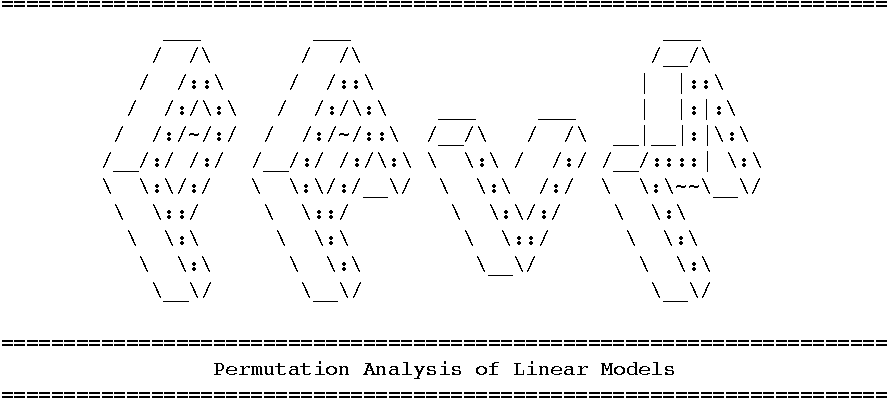
\includegraphics[width=12cm]{figures/palm-logo.pdf}}
%\end{center}
%\caption[Screen shot of \textsc{palm}.]{The methods presented in Chapters \ref{sec:ptree} and \ref{sec:accel} are available in the tool \emph{Permutation Analysis of Linear Models} (\textsc{palm}), a text-based application that can be invoked from scripts.}
%\label{fig:concl:palm-logo}
%\end{figure}


\cleardoublepage \appendix
\cleardoublepage \chapter{Supplementary Material}
\label{sec:supplmat}
\setstretch{\lspac}

The multiplicity of scenarios evaluated in Chapters~\ref{sec:accel} and \ref{sec:cortex} resulted in the construction of more than 40 thousand plots and maps, which do not fit the thesis format; a selection of a few results would unduly overemphasise certain aspects at the expense of others. Instead, we organised these plots in a browsable set of pages, and packaged them into a single, 9.7~\textsc{gb} file that can be downloaded and browsed locally. This file is deposited for long term preservation and public access at the Research Archive of the Bodleian Libraries (\textsc{ora}-Data), and it constitutes the Supplementary Material that accompanies this thesis, accessible under the Digital Object Identifier (\textsc{doi}): \href{http://dx.doi.org/10.9999/xyz}{10.9999/xyz}.\footnote{{\emph{\color{orange}\textsc{note for the assessors}: The \textsc{doi} will be produced should the thesis be approved.}}} The results shown in the thesis make ample reference to this material, and its inspection is encouraged. Mirrored copies that does not require download of a large file, though not guaranteed for long term preservation, can be found at:

\begin{itemize}
\item Chapter~\ref{sec:accel}: \href{http://fsl.fmrib.ox.ac.uk/analysis/fastpval}{fsl.fmrib.ox.ac.uk/analysis/fastpval}
\item Chapter~\ref{sec:cortex}: \href{http://fsl.fmrib.ox.ac.uk/analysis/npcvol}{fsl.fmrib.ox.ac.uk/analysis/npcvol}
\end{itemize}

These links correspond to the Supplementary Materials of the papers related to these two chapters, i.e.,  \citet{Winkler2016_fast} and \citet{Winkler2016_joint}, respectively.
\cleardoublepage
\addcontentsline{toc}{chapter}{References}
\setstretch{1}
\bibliography{biblio}
\pagestyle{empty}
%\cleardoublepage % ======[BLANK]======
%\newpage
%\pagestyle{empty}
%\vspace*{\fill}

\cleartooddpage
\cleartoevenpage[\thispagestyle{empty}]
\thispagestyle{empty}
\vspace*{\fill}
\begin{center}

\includegraphics[width=12mm]{figures/seh_crest_2013.jpg}\\[2mm]
\begin{large}
{\color{teddy}\textbf{St.\ Edmund Hall}}
\end{large}
\end{center}
\end{document}          
